%% Thesis Template of Chinese Academy of Sciences
%%   for using CASthesis package with LaTeX2e
%%
%% Created by Ling-Yun Wu <aloft@ctex.org>
%%
%% Version 0.1 (2004-08-15)
%% Modified by Lei Zhao, 2010-04-10
\expandafter\def\csname CTEX@spaceChar\endcsname{\hspace{1em}}
\documentclass[openany]{SUDAthesis}
\usepackage{xeCJK}
\usepackage{cite}
\usepackage{pdfpages}
\usepackage{tabularx}
\usepackage[normalsize,center]{caption2}
\usepackage{listings}
\usepackage{longtable}
\usepackage{colortbl}
\usepackage{graphicx}
\usepackage{multirow}
\usepackage{subfigure}
\usepackage{stmaryrd}
\usepackage{txfonts}
\usepackage{mathrsfs}
\usepackage{enumerate}
\usepackage[linesnumbered, ruled, vlined, shortend]{algorithm2e}

\renewenvironment{quote}{\vspace{2ex} \newline \kaishu “}{”  \vspace{2ex} \newline }

% algorithm2e使用
\renewcommand{\contentsname}{目\CASTspace 录}
\renewcommand{\listfigurename}{插\CASTspace 图}
\renewcommand{\listtablename}{表\CASTspace 格}
\renewcommand{\listalgorithmcfname}{算\CASTspace 法}
\renewcommand{\algorithmcfname}{算法}

\newcommand{\tabincell}[2]{\begin{tabular}{@{}#1@{}}#2\end{tabular}}

% 参考文献上标格式定义
\newcommand{\ucite}[1]{\textsuperscript{\cite{#1}}}
\numberwithin{algocf}{chapter}
\renewcommand{\thealgocf}{\arabic{chapter}-\arabic{algocf}}


\graphicspath{{../figures/}}

\begin{document}

%% 小节标题靠左对齐(必须在 \begin{document} 之后,否则无效}
\CTEXsetup[format+={\flushleft}]{section}

%%%%%%%%%%%%%%%%%%%%%%%%%%%%%%
%% 封面部分
%%%%%%%%%%%%%%%%%%%%%%%%%%%%%%
  % 中文封面内容
  \title{知识关联网络驱动的语义关联度计算方法的研究}
  \author{李佳鹏}
  \advisor{赵雷}
  \degree{硕~士~}
  \major{计算机科学与技术}
  \minor{计算机科学与技术}
  \submitdate{2020年3月}
  \grade{2~0~2~0~届}

  % 英文封面内容
  \englishtitle{Measuring Semantic Relatedness with Knowledge Association Network}
  \englishAbstractTitle{Measuring Semantic Relatedness with Knowledge Association Network}
  \englishfancytitle{Measuring Semantic Relatedness with KAN}
  \englishauthor{Jiapeng Li}
  \englishadvisor{Lei Zhao}

  % 封面
  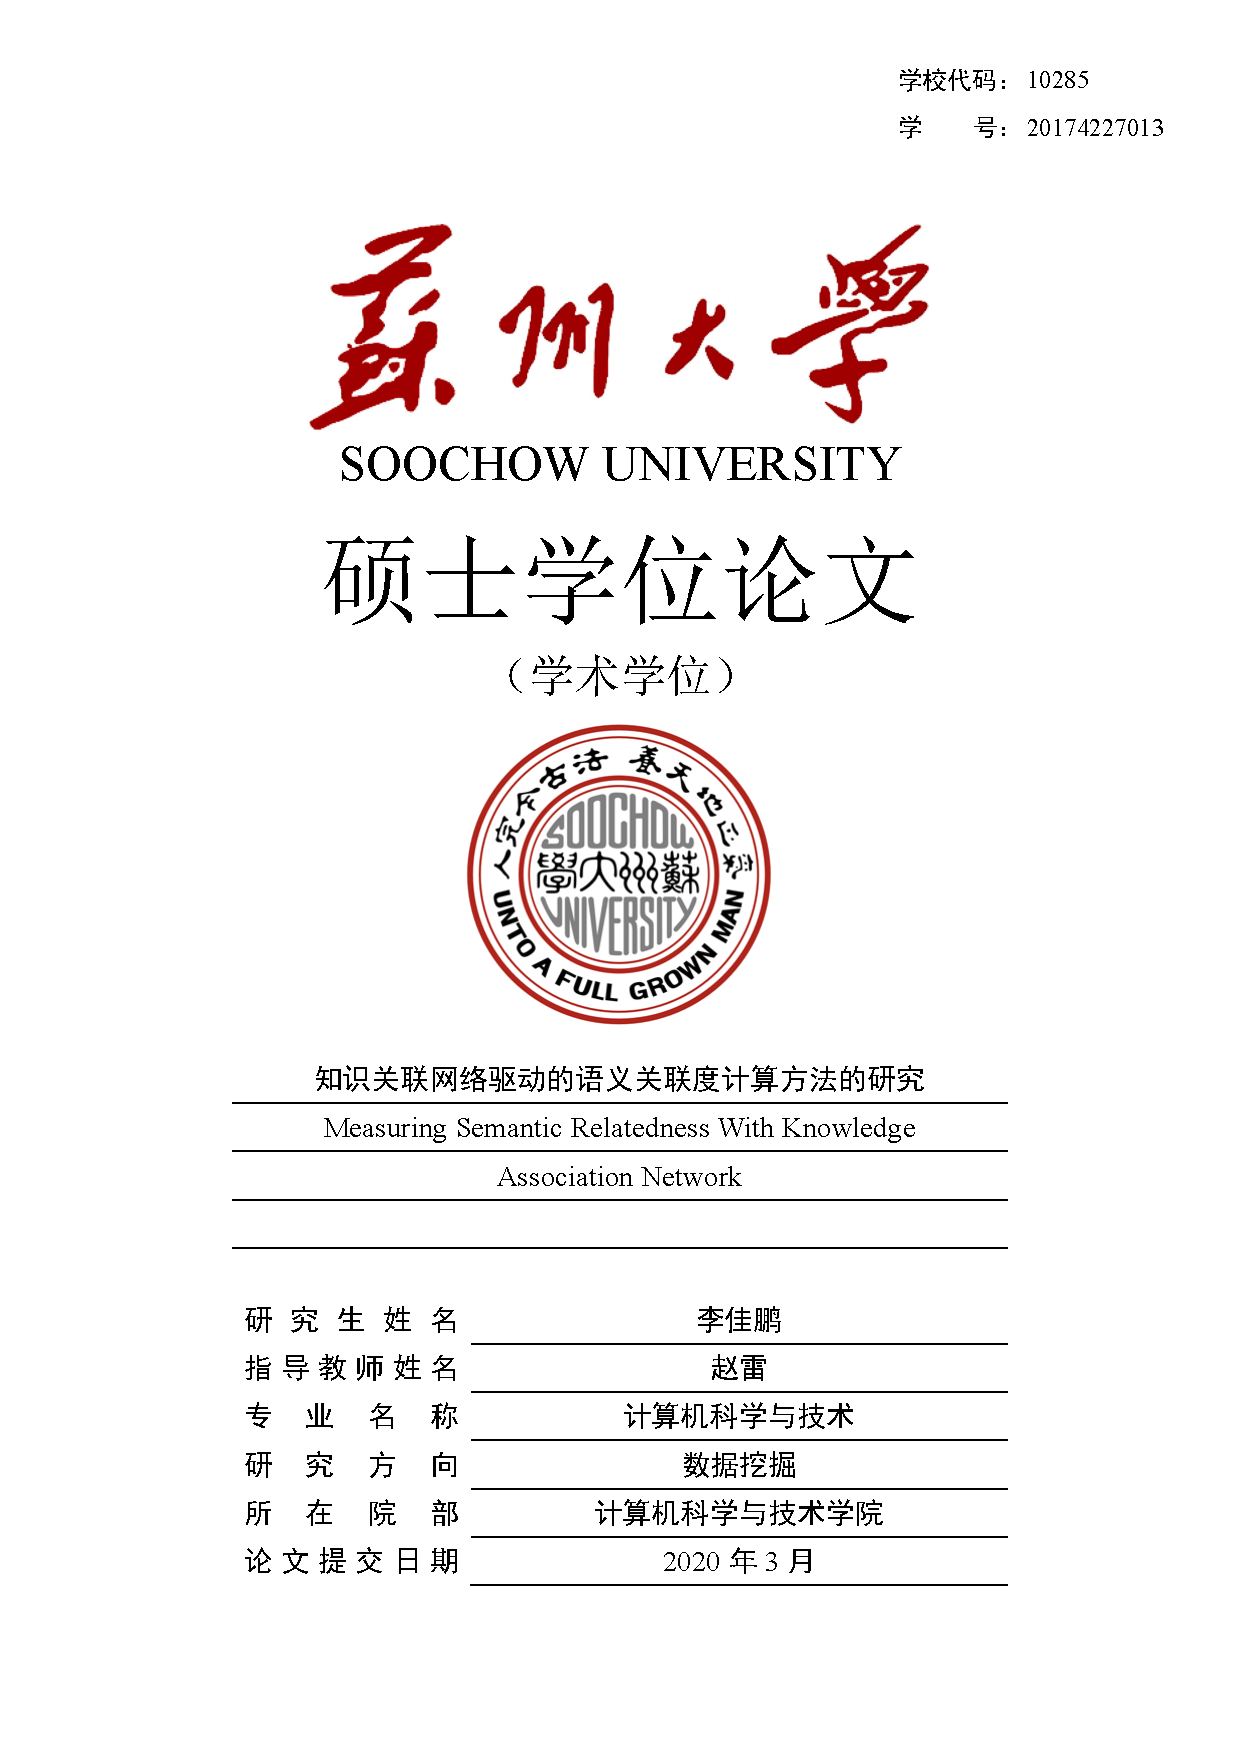
\includepdf{cover.pdf}
  \cleardoublepage

  % 版权页
  %\CopyrightPage
  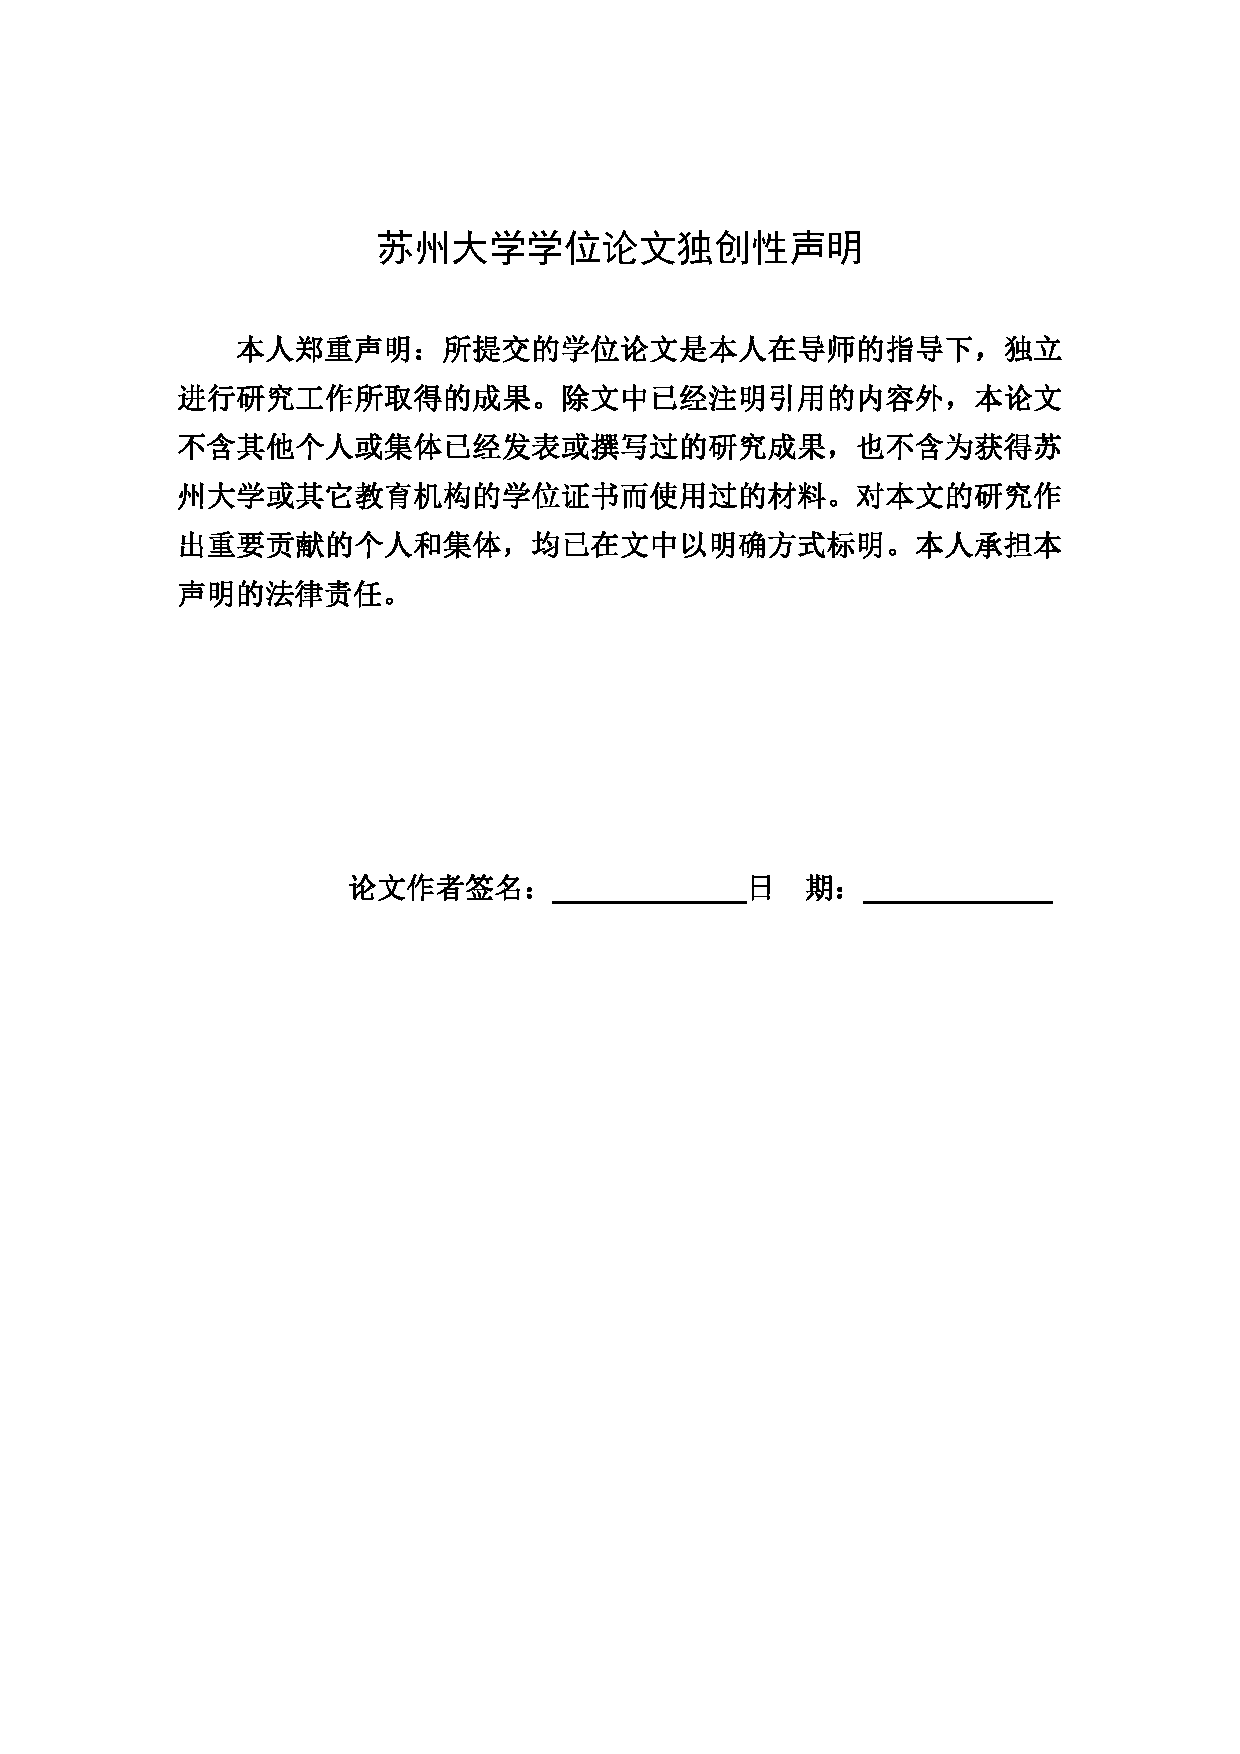
\includepdf{copyrightPage1.pdf}
  \cleardoublepage
  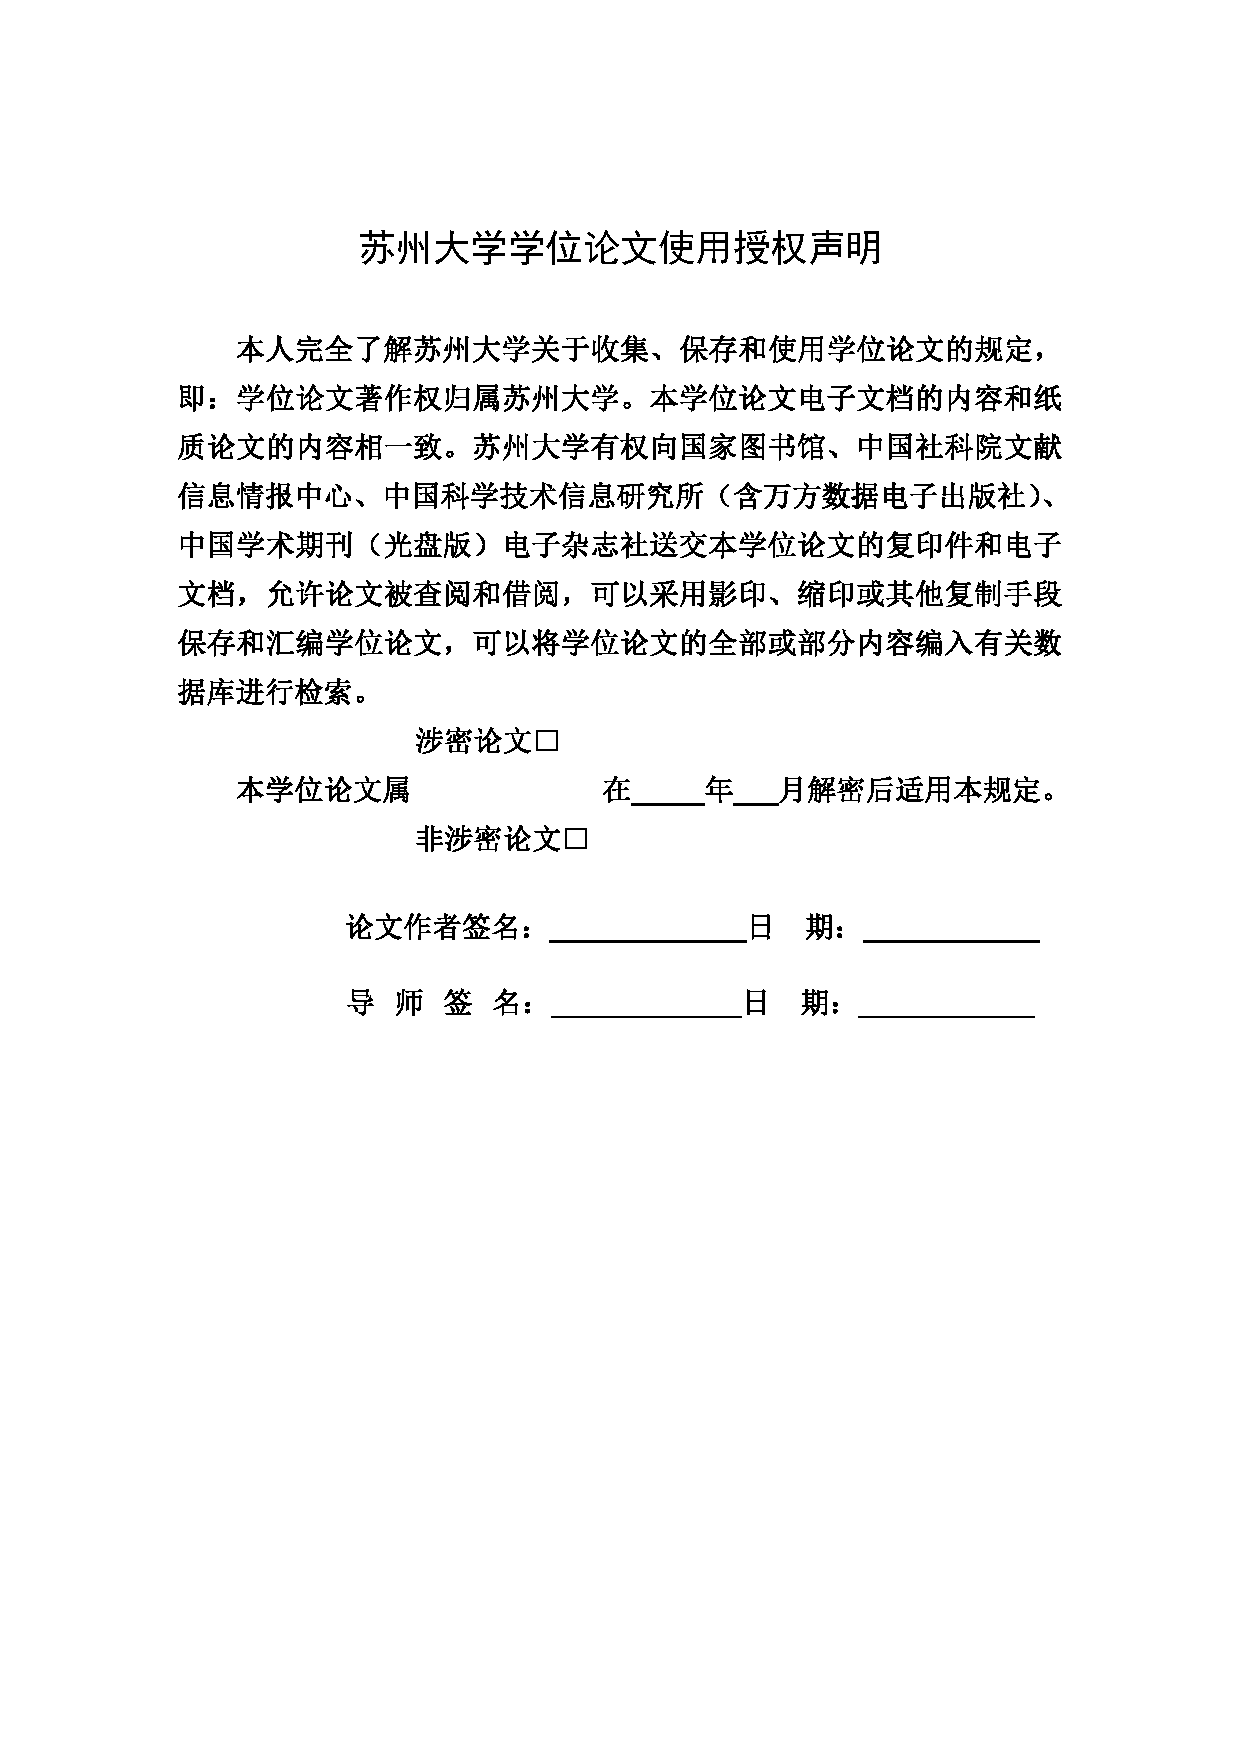
\includepdf{copyrightPage2.pdf}
%%%%%%%%%%%%%%%%%%%%%%%%%%%%%%
%% 前言部分
%%%%%%%%%%%%%%%%%%%%%%%%%%%%%%
  \frontmatter

  % 中英文摘要
  \setAbstractStyle
  \begin{abstract}

    % 所谓语义关联度计算,是指对于给定的一对评测对象,采用合适的方法,结合不同的背景知识,给出一个数值来表示两个对象在语义空间上的关联程度。这两个对象或者是文本中的词语,或者是两个商品,又或者是搜索关键词与文档,从评测对象来看,语义关联度计算是一项基础且十分重要的任务,在自然语言处理、推荐系统和计算机视觉方面都有相关的应用。其中词语之间的语义关联度计算吸引了很多研究者的兴趣。经典的计算方法主要利用了隐含在词典库或文本语料中的隐含语义关系来描述词语语义空间,取得了不错的效果。然而这些方法忽略了隐含在词语背后的语义网络,近年来,新提出的基于自由关联网络的方法改善了这个缺点,在语义关联度计算方面取得了更好的效果。但是这种方法需要事先对Wikipedia进行大量的复杂的预处理,此外,这种方法采用了固定的评分函数来衡量Wikipedia页面之间的相关性,这造成了模型灵活性和表达能力的欠缺。

    所谓语义关联度计算,是指对于给定的一组词语,用一个数值来表示两个词语在语义空间上的关联程度。此任务在自然语言处理和推荐系统中扮演着十分重要的角色,也吸引了很多研究者的兴趣。经典的计算方法主要利用了隐含在词典库或文本语料中的语义关系来描述词语语义空间,取得了不错的效果。然而这些方法忽略了词语所关联的语义网络,近年来新提出的基于自由关联网络的方法改善了这个缺点,取得了更好的效果。但是这种方法需要事先对文本语料进行复杂的预处理,且其采用的固定启发式函数造成了模型灵活性和表达能力的欠缺。

    为了改善传统自由关联网络方法中遇到的问题,本文根据词语与不同知识图谱实体之间的关系来建立知识关联网络,由此避免了复杂的文本预处理,同时本文采用了网络嵌入的方式来学习更加灵活鲁棒的知识表示,由此提升语义关联度计算的表现,具体来讲,本文的研究内容包含两个部分。

    (1)WordNet关联网络驱动的语义关联度计算。本文利用词语与WordNet实体间的关系构建WordNet关联网络。然后采用基于自注意力机制的网络嵌入模型来得到WordNet实体的词法向量表示。基于标准测评数据的实验结果表明,基于自注意力机制的网络嵌入模型可以更好得学习到实体的向量表示。此外,通过结合WordNet实体词法向量与文本语料上训练得到的词向量,可以更好地提升模型效果。

    (2)DBpedia关联网络驱动的语义关联度计算。本文基于TF-IDF思想建立起词语与DBpedia之间的关联,旨在利用实体之间的关系来丰富词语的语义信息。此外本文还提出了一种灵活的具有表达力的模型来学习词语背后的关联实体表征,这种模型同时将实体所处的属性空间与拓扑结构空间表示映射到向量空间,提高了模型的表达力。实验结果证明,此模型进一步提高了语义关联度计算的评测效果。

    相对于传统的自由关联网络,本文利用知识图谱构建的知识关联网络避免了复杂的文本预处理,同时本文针对基于不同知识库构建的知识关联网络给出了计算过程,相对于人为设计的启发式函数,本文提出的网络学习过程也更加灵活鲁棒,并取得了不错的效果。

\keywords{语义关联度,知识图谱,网络嵌入}

\end{abstract}

\vspace{-6.4pt}
\soochowauthor{李佳鹏~\quad}

\soochowtutor{赵~~~~雷\quad}


  \newpage
  \thispagestyle{empty}
  \setEnAbstractStyle
  \begin{englishabstract}

    % Measuring semantic relatedness is suggested to produce a score which indicates how two objects are related. The objects can be words in texts, or goods, or search words and documents, follows that semantic relatedness measurement is a fundamental task for many applications in natural language processing, recommendations and computer vision domains. Many researchers pay attention to semantic relatedness computing between words.Conventional methods mainly utilize the latent semantic information hidden in lexical databases or text corpus to compute semantic relatedness and make great achievements. However these methods ignore the semantic network behind words. Recently, some other approaches have made great efforts based on free association network and achieved a significant improvement on relatedness measurement. Nevertheless, they need complex preprocessing in Wikipedia. Besides, the fixed score functions they employ cause the lack of flexibility and expressiveness of model. 

    Measuring semantic relatedness is suggested to produce a score which indicates how two words are related. This task plays a very important role in natural language processing and recommendation system, and also attracts many researchers' interest. Conventional methods mainly utilize the latent semantic information hidden in lexical databases or text corpus to compute semantic relatedness and make great achievements. However these methods ignore the semantic network behind words. Recently, some other approaches have made great efforts based on free association network and achieved a significant improvement on relatedness measurement. Nevertheless, they need complex preprocessing in Wikipedia. Besides, the fixed heuristic functions they employ cause the lack of flexibility and expressiveness of model. 

    To remedy the weaknesses of free association network-based methods, this paper constructs Knowledge Association Network based on the relationship between words and different knowledge graphs. Moreover, to improvement the performance of semantic relatedness measurement, this paper uses the way of network embedding to learn flexible and robust knowledge representation. Specifically, this paper contains two parts.
  
    (1) Measuring semantic relatedness with WordNet Association Network. This paper utilizes the relationship between words and entities in WordNet to construct the Association Network. Then we get the lexical vector representation of entities by network embedding models. The experiment results based on standard datasets show that the network embedding model based on self attention can better learn the vector representation of entities. Moreover, we can get better performance by combining vector of entities and word vector based on text corpus(Wikipedia).
  
    (2) Measuring semantic relatedness with DBpedia Association Network Representation Learning. This paper constructs the relationship between words and entities in DBpedia based on the idea of TF-IDF. We leverage the relatedness among entities to enrich the semantic information of words. We also propose a flexible and expressive model to represent entities behind the words, in which attribute and the topological structure information of entities are embedded in vector space simultaneously. The experiment results based on standard datasets show the better effectiveness of our model compared to previous models.

    Compared with the traditional free association network, the knowledge association network constructed based on the knowledge graph avoids the complex text preprocessing. At the same time, this paper gives the calculation process for the knowledge association network constructed by different knowledge bases. Compared with the heuristic function designed by human, the network learning process proposed in this paper is more flexible and robust, and has achieved good results.

\englishkeywords{Semantic Relatedness, Knowledge Graph, Network Embedding}

\end{englishabstract}

\ensoochowauthor{~Jiapeng Li~\quad }

\ensoochowtutor{Lei Zhao\quad}


  \newpage
  \cleardoublepage
  \thispagestyle{empty}

  % 目录
  \setContentsStyle
  \tableofcontents
  % 插图目录
  \listoffigures
  % 表格目录
  \listoftables
  % 算法目录
  \listofalgorithms

%先定义好环境变量名称
%\newtheorem{observation}{观察}
%\newtheorem{PruneStrategy}{剪枝规则}
\newtheorem{definition}{定义}
\newtheorem{lemma}{引理}
\newtheorem{theorem}{定理}
\newtheorem{pf}{证明}
\newtheorem{code}[thm]{代码}
\newtheorem{RULE}{规则}
\newtheorem{example}{例}

%%%%%%%%%%%%%%%%%%%%%%%%%%%%%%
%% 正文部分
%%%%%%%%%%%%%%%%%%%%%%%%%%%%%%
\mainmatter

  \setstyle
  \xiaosihao

  \chapter{绪论}
\label{chap:chap01}

\section{研究背景和意义}
在现实科研生活中,研究者们经常会遇到的一个问题是: 如何衡量两个具象事物或者抽象概念之间的相关程度。在计算机视觉(Computer Vision, CV)方面,有研究者通过研究词语与图片之间的关联程度来挖掘图片中存储的隐含语义\cite{iwcs/LeongM11}; 在生物医学中,研究者们需要去比较基因或者蛋白质之间的功能差异,由此来构建生物医学知识系统~\cite{bib/GuzziMGC12,bmcbi/BenabderrahmaneSPND10};在地理学中,衡量两个地理学概念之间的差异与联系贯穿于整个地理学系统中~\cite{josis/JanowiczRK11};自然语言处理(Natural Language Processing,NLP)中,大量任务需要比较两个对象之间的关联度,例如:命名实体识别中需要衡量候选实体集与目标实体之间的近似度~\cite{acl/HanZ10},关键词抽取中需要评价候选关键词与文章的关联度~\cite{ijcai/ZhangFW13},文本关联度度量任务需要评估句子或者文档之间的相似度~\cite{ijcai/YazdaniP13}等等。

上述谈到的任务通常会涉及到词语之间的语义关联度(Semantic Relatedness)度量,所谓语义关联度,是指对于给定的一对单词,通过比较其语义表征来给出其背后包含的意义或其语义内容之间的相关程度。很多研究者经常不区分语义关联度与语义相似度(Semantic Similarity)之间的差异,语义相似度是指词语之间种属(is-a)关系的相似度,而语义关联度包含语义相似度,指考虑词语之间的所有关系(种属、反义、部分整体等)之后给出的词语间关联程度~\cite{geoinformatica/BallatoreBW14}。举个例子来说\emph{actor(演员)}跟\emph{person(人)}相似,但是跟\emph{movie(电影)、Hollywood(好莱坞)}相关联而不相似。

\begin{figure}
    \centerline{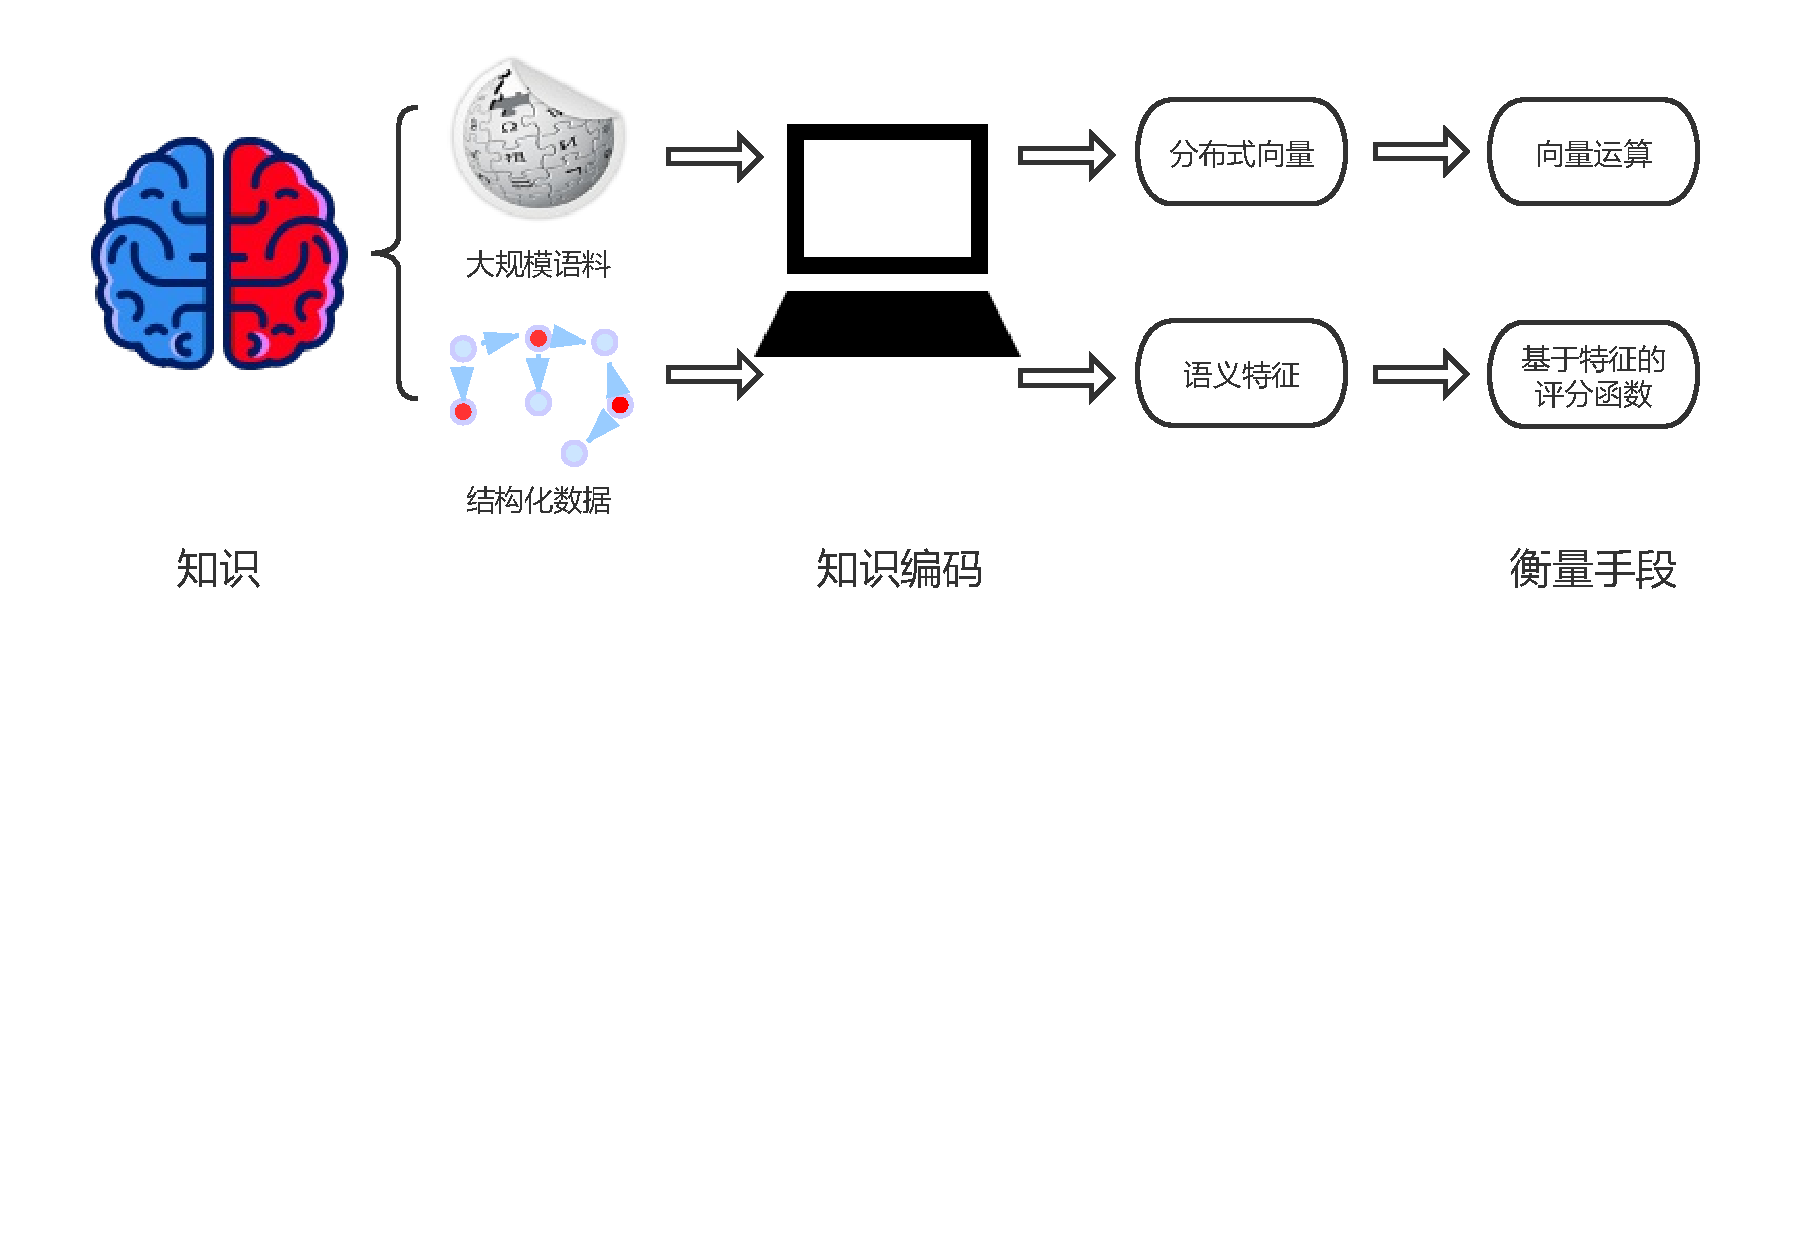
\includegraphics[width=1\textwidth]{chap1-1.pdf}}
    \smallcaption{语义关联度度量简单过程}
    \label{chap1-1}
\end{figure}

对于语义关联度度量,人类会结合自身的认知、经验等来主观并直接地判断两个词语背后包含的知识、意义等之间的相关程度。但是对于计算机来说,如图~\ref{chap1-1},这显得没有那么容易,面临着以下问题:1)知识编码:包含在比较对象中的先验知识无法被简单地转化为数值,无法直接地作为计算机系统的输入;2)衡量手段:当我们可以编码两组对象背后隐含的知识并输入到计算机系统时,针对不同的知识编码方式,采用何种衡量手段来评估语义关联度度量效果也是一个值得研究的问题。

知识的编码往往依赖于知识的存储形式。如表~\ref{knowledge-base}所示,在过去的十几年里,研究者们主要利用以下几种知识存储形式来挖掘词语的意义或语义内容:1)自然语言大规模语料:互联网中存储着丰富的由专业人才构建的高质量自然语言文本,如新闻语料,维基百科\footnote{https://www.wikipedia.org/}等,这些语料中词语的共现信息、词语的上下文信息等都反映了词语的语义内容,因此大规模规范化语料是研究者常利用的一种知识存储形式。2)结构化的知识库:主要包含本体库(Ontology),知识图谱(Knowledge Graph,KG)等,这里作简要介绍:
%
i)在计算机科学与信息科学领域,本体是指一种“形式化的,对于共享概念体系的明确而又详细的说明”~\cite{ka/GRUBER1993199},这是一种直观的形式化的存储形式,反映了领域内知识的层次结构,更加适合在计算机系统中使用,常用的本体库有OWL\footnote{https://www.w3.org/TR/owl-features/}等;
%
ii)大规模语料中的语义信息往往以非结构化或者半结构化的形式存储,为了直观的描述和存储知识,研究者们结合机器抽取和人为标注的方式建立高质量知识图谱,其以三元组(triple)的形式,如WordNet\footnote{https://wordnet.princeton.edu/}、DBpedia\footnote{https://wiki.DBpedia.org/}等,存储着多种多样的实体以及它们之间的关系。通过这样的形式,将知识转化为图结构,方便了后续知识推理、信息检索、语义挖掘等任务的进行。

\begin{table}[!ht]
    \center
    \smallcaption{常用的知识存储形式}
    \vspace{5pt}
    \begin{tabular}{|c|c|c|c|l}
        \cline{1-4}
            & 存储结构 & 主要存储形式 & 实例 & \\ \cline{1-4}
        结构化知识库 & 本体库、知识图谱 & 三元组、图结构 & OWL、WordNet、DBpedia & \\ \cline{1-4}
        大规模语料 & 文本 & 自然语言 & 维基百科 & \\ \cline{1-4}
    \end{tabular}
    \label{knowledge-base}
\end{table}

针对这些知识存储形式,研究者们从下面几个方面入手挖掘知识库中包含的语义信息,由此来完成语义关联度度量:
%
1)基于词法信息的度量方法:研究者们利用WordNet~\cite{acl/Pucher07, tkde/ZhuI17}和Wikitionary~\cite{aaai/ZeschMG08}等知识库来衡量词语间的关联度。他们通过计算知识库中实体之间的路径距离来反映词语间的关联度,距离越近两个词语之间的关联度越高。这种方法在语义相似度衡量任务上表现要优于关联度度量,较好地反映了词语在词法空间或者词语层次结构上的距离,但是由于本体库本身仅仅存储了一些人为构建的词语间层次种属关系,这种方法自然也就无法考虑到词语在语义空间上的信息。
%
2)基于共现原则的度量方法:这种方法认为共同出现在一个句子或窗口中的两个词之间是相关的。大规模自然语言文本中包含着丰富的共现语义信息,为了更全面准确地衡量词语间语义关系,研究者们或从文本中抽取词语之间的关系~\cite{aaai/Milne08},或利用语义分析学习词向量~\cite{ijcai/GabrilovichM07, corr/Mikolov13, emnlp/PenningtonSM14},并且比基于本体库的度量方法取得了更好的效果。但是对于同义词来说,他们几乎不会同时出现在一个句子中,而且共同出现的单词之间也会发生偶发性的不相关现象。
%
3)基于关联网络的方法~\cite{aaai/ZhangZH15, aaai/GongXH18}:为了改善基于共现原则的方法中遇到的问题,这种方法考虑了单词背后的关联实体对关联度度量结果的影响。关联网络最早起源于心理学实验,研究者认为给定一个词,第一个出现在受试者脑海中的词是与给定词最相关的。基于这样的假设,研究者们通过建立关联网络来连接词语与Wikipedia中的实体,由此来丰富词语的语义信息。在建立好的关联网络中,以往的研究中采用大量的启发式评分函数来计算实体之间的语义关联度,再利用此计算结果优化词语间的关联度计算。这种方法虽然在基于大规模语料的统计分析方法基础上,提升了实验性能,但是还面临着一些不足:a)固定的基于规则的启发函数缺乏扩展性和灵活性;b) 对于词语背后的实体关联度比较,这种方法基于规则地从Wikipedia中抽取大量的实体共现信息,实体属性信息以及实体之间的链接信息等,这需要大量复杂的文本预处理。

如上文所述,结构化的知识库中包含着由机器抽取和人为标注构成的高质量信息,本文通过建立词语与知识库实体之间的关联来规避对大规模语料的预处理,其中由词语、知识库实体所构成的网络,我们称之为知识关联网络(Knowledge Association Network,KAN)。对于知识关联网络中的知识库实体,本文通过网络嵌入的方法来学习其分布式向量表示。这种低维的表示可以将实体的多种不同语义信息映射到同一向量空间,然后通过简单高效的向量运算得到实体之间的关联程度。


\section{研究内容}
世界上的各种事物往往都存在各种各样的联系,对于某一种具象事物,其背后往往有多种抽象概念与之对应。图\ref{chap1-2}反映了词语和相关联的实体所构成的网络结构。在这种结构中存在三种关系:
%
1)词语与词语的关系:是指对于给定的一段文本和一个固定大小的窗口,在同一个窗口内出现的词语之间具有联系,这反映了词语与词语的共现关系;
2)实体与实体的关系:词语背后的关联实体作为一种语义补充,在知识库在中表征为有向图,反映了各种实体之间的种属层次关系;
3)词语与实体的关系:对于一个词语,其和不同实体之间的关联程度也是不同的。
%
当利用实体之间的关系来丰富词语的语义信息,并由此来更好地计算词语间的语义关联度时,需要综合考虑这三种关系对结果的影响。面临的第一个问题是如何构建知识关联网络;第二个问题是对于不同的网络形式和规模,如何计算词语间语义关联度。

\begin{figure}
    \centerline{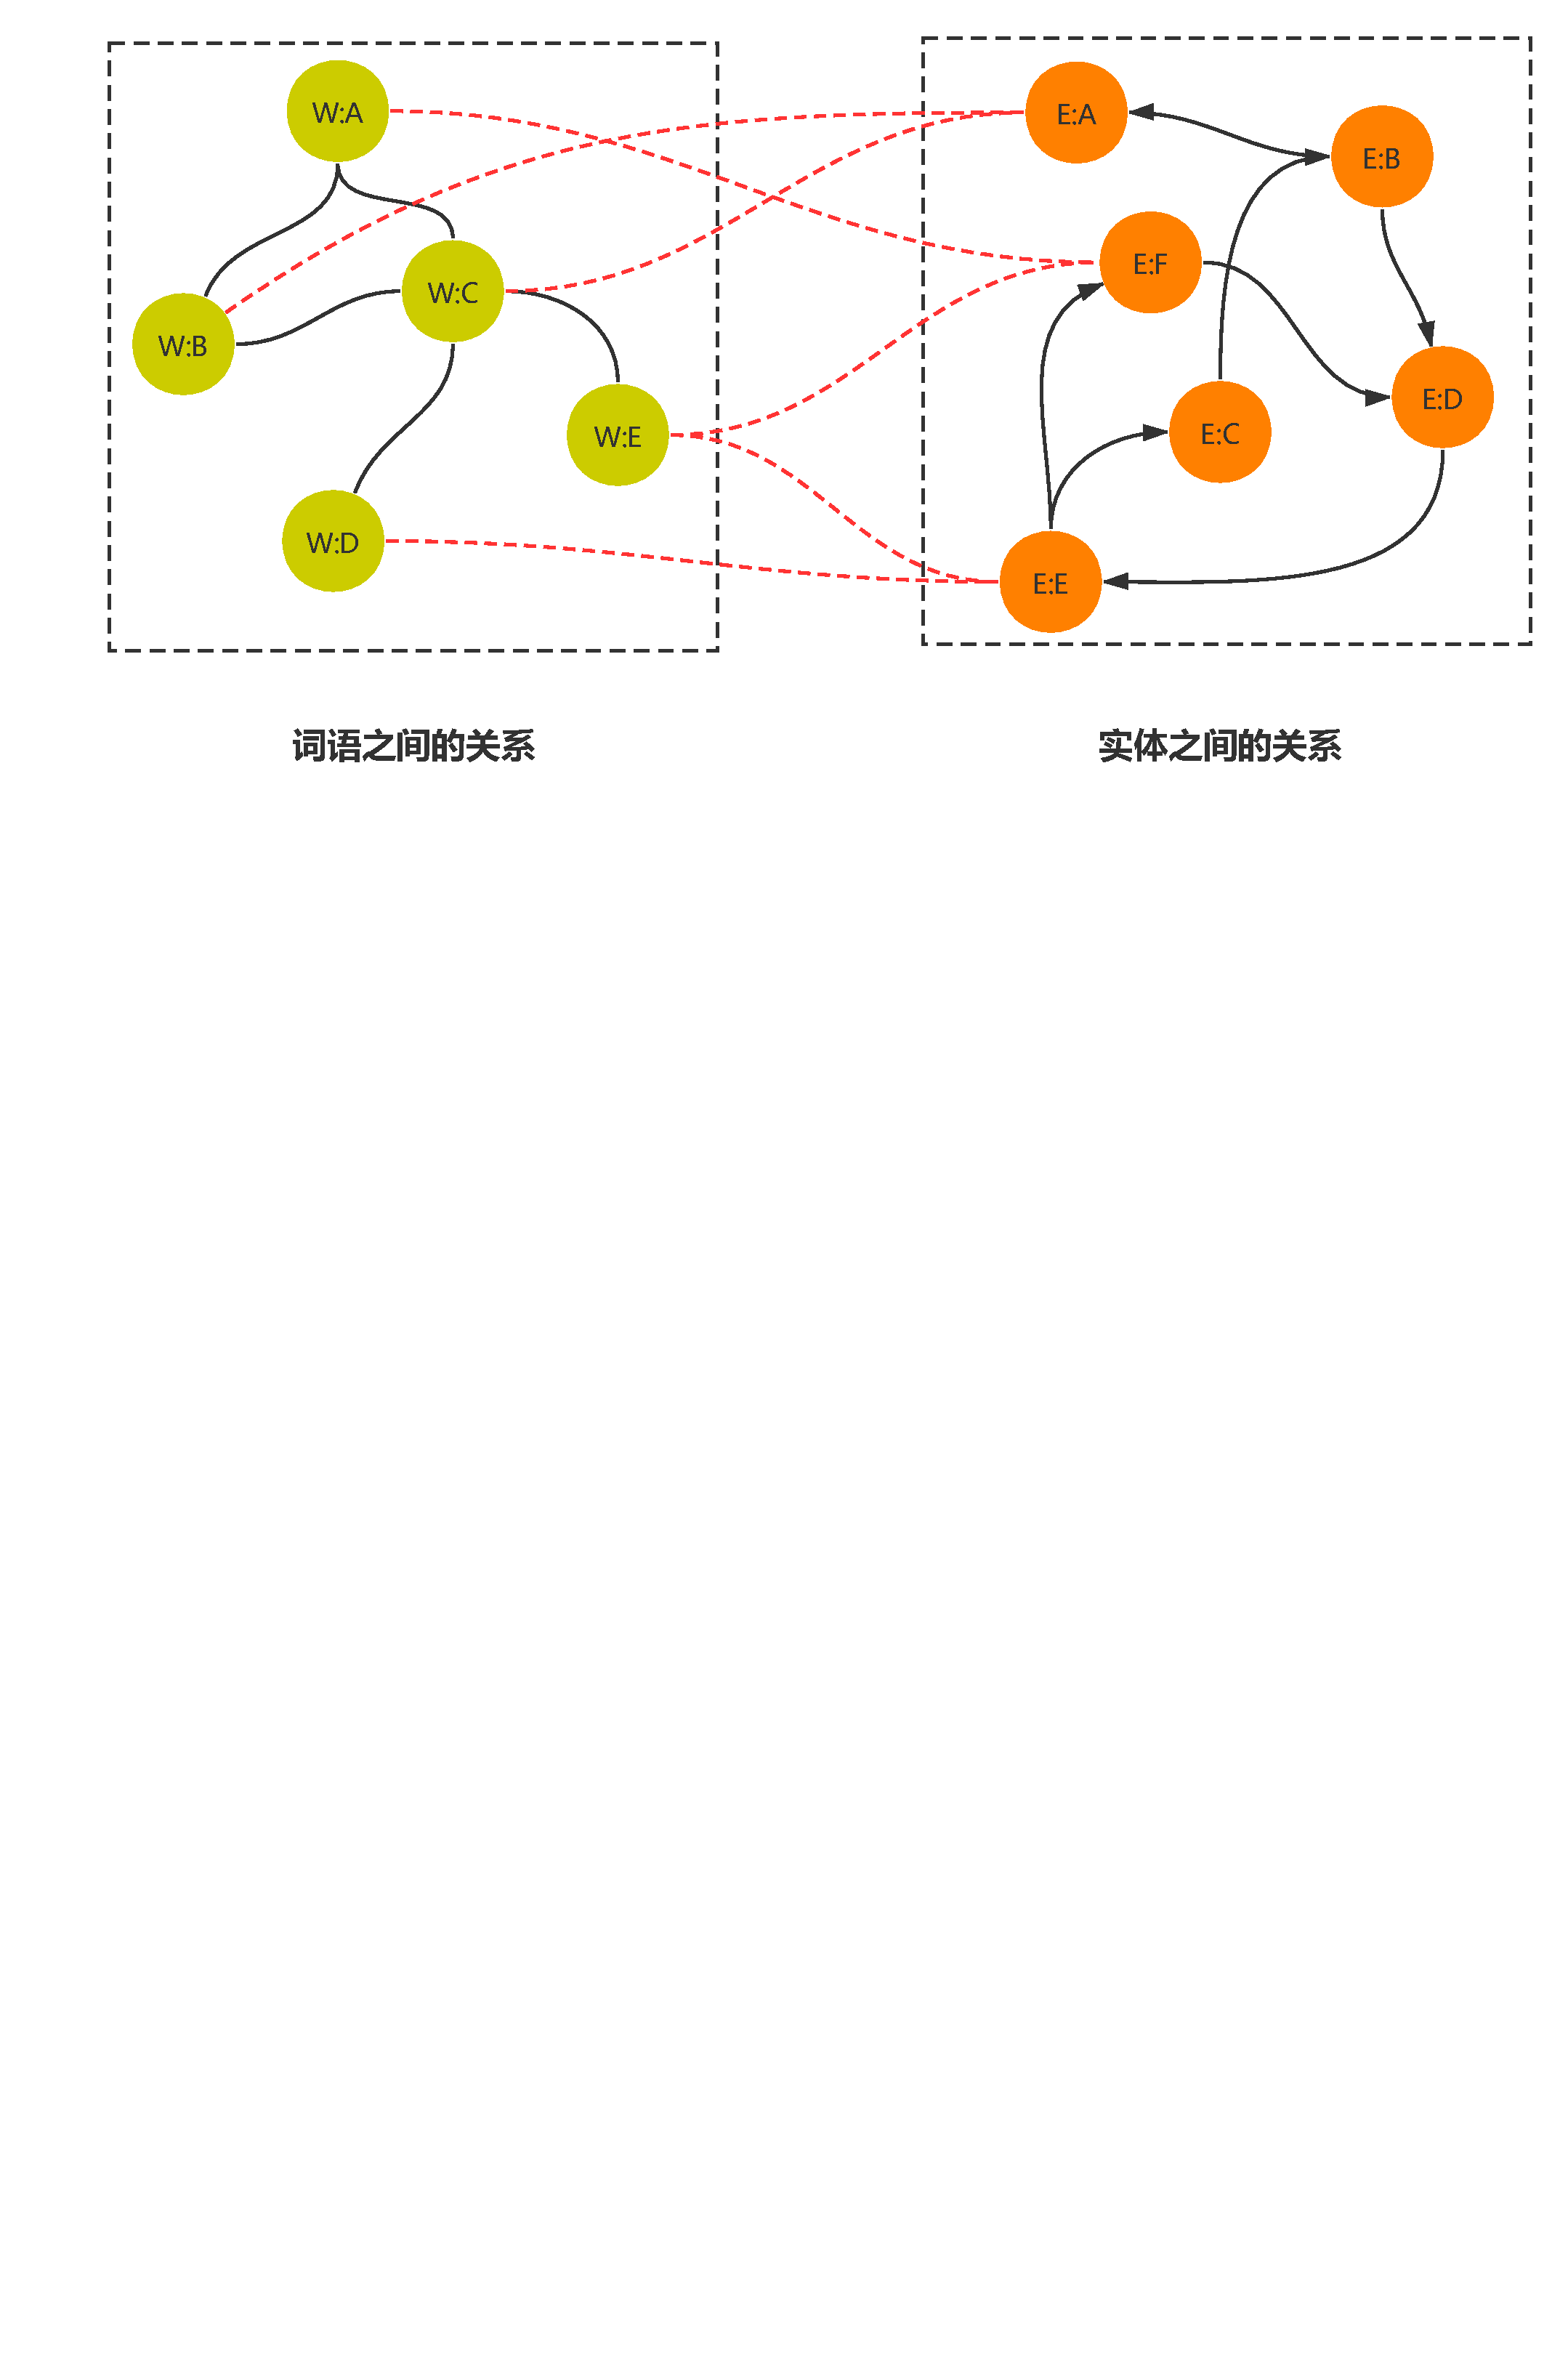
\includegraphics[width=0.8\textwidth]{chap1-2.pdf}}
    \smallcaption{词语和与其相关的知识库实体构成的知识关联网络}
    \label{chap1-2}
\end{figure}

针对第一个问题,即如何构建知识关联网络?其关键是如何建立词语与实体之间的对应关系。对于不同的知识库,建立词语与实体之间关联的方式不同。本文考虑了两种知识库来建立知识关联网络:
1)WordNet作为一种英文词法关系库,其按照单词之间的语义内容和词法关系,将大量英文单词划分为一组组同义词集(synsets),其中包含175979个同义词集和155327个词语,每个同义词集集代表了一个唯一的概念。每个词语与同义词集之间的对应关系也被人为严格准确的标注好并保存在其中,这使得词语与同义词集之间的对应关系可以通过词语字面值匹配被查询到;
2)DBpedia是从维基百科中构建得来的高质量知识图谱,其中每个实体对应于一个维基页面描述的对象。至2016年10月,DBpedia中包含了约600万实体和13亿条RDF三元组\footnote{https://blog.dbpedia.org/2016/10/19/yeah-we-did-it-again-new-2016-04-dbpedia-release/} 。但是DBpedia中没有直接存储词语与实体之间的对应关系,文本首先建立词语与维基页面之间的关系,然后利用实体与维基页面之间的一一对应关系对应到DBpedia中的实体。

第二个问题是在知识关联网络驱动下如何计算语义关联度。本文考虑知识关联网络中包含的三种关系,利用实体层的语义信息来加强词语间的语义关联度度量,而词语与实体之间的关系起到连接词语层和实体层的作用。对于词语层之间的语义关联度度量,本文保留了传统关联网络中的方法,利用词向量~\cite{corr/Mikolov13, emnlp/PenningtonSM14}模型将大规模语料中词语之间的共现关系表示为分布式向量,由此来获得其语义特征。而对于实体层的语义关联度度量,本文分别针对两种不同方式构建的知识关联网络,采用了不同的方法来学习网络实体表示:
\begin{enumerate}
    \item 基于WordNet的知识关联网络驱动的语义关联度计算:WordNet中的实体(同义词集)关系表现为有向图的形式,传统的图注意力网络(Graph Attention Network, GAT)\cite{iclr/VelickovicCCRLB18}多用在有监督或半监督的节点分类任务上,本文提出采用无监督模式的图注意力机制来学习WordNet中实体的分布式向量表示。基于标准测评数据集的实验结果表明,无监督自注意力机制的网络嵌入模型可以更好地学习到实体的向量表示。此外,通过结合WordNet词法向量与文本语料上训练得到的词向量,可以更好的提升模型效果。
    \item 基于DBpedia的知识关联网络驱动的语义关联度计算:DBpedia中的实体数量远超过WordNet中的数量,无监督注意力模型随之变得难以训练。本文将DBpedia中实体的语义信息分为属性空间和拓扑空间,并提出了一种灵活的具有表达力的模型来学习知识图谱中的实体表征。对于实体的属性空间,本文通过最小化正例实体属性对间隔,最大化负例实体属性对间隔的方法来学习其向量表示;而对于实体的拓扑空间,本文首先通过随机游走生成采样序列,然后利用Skip-Gram\cite{corr/Mikolov13}模型去学习实体的向量表示。实验结果证明,此模型进一步提高了语义关联度计算的评测效果。
\end{enumerate}

\noindent 综上所述,本文的贡献有以下几点:
\begin{enumerate}
    \item 本文基于WordNet、DBpedia知识库去构建了知识关联网络,同时考虑了词语与词语、词语与实体以及实体与实体之间的关系对语义关联度度量的影响。
    \item 在知识关联网络的实体层,针对不同的网络结构,本文提出了不同的网络嵌入模型。在基于WordNet构建的网络中,本文将图注意力机制应用到无监督表示学习中;在基于DBpedia构建的网络中,本文同时考虑了实体属性空间与拓扑空间的语义信息。这些分布式向量表示方法在扩展性与灵活性上要明显优于传统模型中人为设计的启发式比较函数。
    \item 基于标准语义关联度度量评测数据集的实验证明,本文的模型要优于几种对比模型,取得了更好的效果。
\end{enumerate}

\section{研究现状}
词语语义关联度计算在生物医学、自然语言处理等应用中扮演者十分基础且重要的角色,其目的是衡量两个词语在语义空间上的距离。本节简要介绍了以往研究者如何利用不同知识表现形式来刻画词语在语义空间上的信息。
%
此外词语背后的语义信息多表现为图的形式,如何更好的将图中信息嵌入到向量空间也是影响关联度度量的关键因素,此外,各种图嵌入模型也在推荐系统,自然语言处理等方面都有重要的应用,本节也将简要介绍了几种常用的图嵌入模型及其应用场景。

\subsection{语义关联度计算的研究现状}
本小节针对不同的知识存储形式,从下面几个方面介绍历史研究者们如何挖掘知识库中包含的语义,如何完成语义关联度度量:

\textbf{基于词法信息的度量方法:}
这种方法基于WordNet和Wikitionary等单词词法库来衡量词语间的语义关联度。WordNet作为一种英文词法关系库,其按照单词之间的语义内容和词法关系,将大量英文单词划分为一组组同义词集。Wikitionary\cite{aaai/ZeschMG08}作为一个人工构造的高质量词法库被提出,旨在为大量的的AI应用提供基础服务。对于一对词语,最早的研究者们\cite{its/Rada89, Leacock98, wu1994verb, tkde/LiBM03}在词法树中找到多条路径连接这两个词,其中最短的一条路径反映了两个词语之间的关联程度。还有一些研究者们,利用WordNet中的同义词集合对应的信息内容(Information Content, IC)值来衡量词语间关联度\cite{ijcai/Resnik95, RCLIC/Jiang97, icml/Lin98},其中IC值被定义为$-log p(c)$,$p(c)$被定义为概念$c$出现在语料库中的频率。由此可见越是具体的概念,比如说“actor”其IC值越高,越是抽象的概念,如“person”其IC值越低。但是这种方法多用来建模词语间的层次关系,在语义相似度方面表现较好,但是对于涉及多种语义关系的关联度度量,这种方法表现不太好。

\textbf{基于共现原则的度量方法:}
为了更好地考虑词语的语义关系,研究者们提出基于词语共现关系来计算语义关联度的方法。即认为在语料文本中,两个词如果共同出现在一个句子或者一个窗口中,则这两个词是相关联的。最初的模型WikiRelate!~\cite{aaai/StrubeP06}利用维基页面中包含的文章类别(Categories)信息来衡量词语间的语义关联度。显式语义分析(Explicit Semantic Analysis,ESA)~\cite{ijcai/GabrilovichM07}首先将维基百科中一篇文章的语义信息表示为高维向量空间,然后通过向量空间的运算来衡量词语间的语义关联度。但是WikiRealted!和ESA仅仅考虑了文本中词语的统计信息,忽略了维基百科中文章之间的链接信息。接下来提出的WLM~\cite{aaai/Milne08}模型利用词语与维基页面中锚文本之间的匹配关系,建立起词语与文章的关系,由此利用文章之间的链接信息提升了词语间语来义关联度度量效果。随后提出的WikiWalk~\cite{textgraphs/YehRMAS09}模型则扩展了WLM模型,进一步考虑维基百科中的页面主体、信息框(infobox)和类别区域中的外链信息建立起文章之间的连接图,然后利用随机游走算法~\cite{emnlp/HughesR07}学习到图中每个节点的向量分布,最后通过向量之间的余弦距离来衡量词语间关联度。SSA\cite{aaai/HassanM11}则利用维基百科中词语上下文中的实体信息为词语构建语义画像,然后通过基于规则的方法计算词语间关联度;Word2Vec\cite{corr/Mikolov13}利用词语之间的共现信息来将词语表征在向量空间,由此来计算语义关联度。

但是上述模型无法有效地建模词语的多种含义,SaSA\cite{aaai/WuG15}利用维基百科词语上下文包含的不同实体为词语分配不同意义,在词义层面学习词语向量表示,解决了Word2Vec中无法表征词语多义性的缺点。而Iacobacci等提出的SensEmbed~\cite{acl/IacobacciPN15}则利用外部知识库BabelNet\footnote{http://babelnet.org}来标注维基语料中词语的不同含义,然后利用Word2Vec~\cite{corr/Mikolov13}模型来学习不同词义的分布式表示。此外,Giuseppe提出的REWOrd模型利用来知识图谱DBpedia和SPARQL查询语言建立起词语与知识图谱之间的联系,由此考虑词语背后的多种含义,然后利用DBpedia中的谓词统计信息来衡量词语之间的语义关联度。

基于共现原则的度量方法有效地考虑词语之间的多种关系,取得了很好的效果。但是对于一些同义词来说,他们几乎不会同时出现在一个句子中,而且共同出现的单词之间也会发生偶发性的不相关现象。接下来要介绍的基于关联网络的度量方法在基于共现方法的基础上利用了词语背后相关的实体中包含的语义信息,有效地提升了度量效果。

\textbf{基于关联网络的度量方法:}
为了改善基于共现原则的方法中遇到的问题,这种方法考虑了单词背后的关联实体对关联度度量结果的影响。关联网络最早起源于心理学实验,研究者认为给定一个词,第一个出现在受试者脑海中的词是与给定词最相关的。基于这样的假设,Keyang~\cite{aaai/ZhangZH15}等人扩大词汇覆盖范围,并通过构造一个词语和概念的关联网络来克服稀疏性,将自由联想(Free Association)规范中的信号和从维基百科的丰富结构中提取的五种类型的共现相结合,这种方法在词语和短文本关联度量中取得不错的效果。Xiaolong\cite{aaai/GongXH18}等人随后提出层次关联网络(Hierarchical Association Network ,HAN)的结构去捕捉词语和Wikipedia实体概念之间的复杂关系,并针对每种关系采用合适的度量方法。通过这种方法,他们取得更好的度量效果。但是,在实体关系比较的过程中,这种模型通过人工设计的特征和固定的统计评分函数去计算实体之间的语义关系。此外,为了得到实体的语义信息,这种方法需要对Wikipedia进行大量的复杂预处理。

文本提出的知识关联网络驱动的语义计算,利用结构化知识库去丰富词语层语义信息,避免了对大规模语料的预处理。同时,本文通过分布式向量表征来表示实体的语义空间,有效地改善了传统手工特征抽取和固定评分函数的不足,取得了不错的度量效果。

\subsection{图嵌入的研究现状}
图作为一种更加普适的结构,反映了各种事物之间的联系,自然界万物之间的关系可以构成一张大图。如何更好地表示的图中的信息成为了各路研究者前仆后继的目标。其中网络嵌入是指根据网络中节点或边所处的网络结构和属性信息,通过一系列技术手段将网络节点或边的各种信息表示在低维向量空间,从而方便后续节点聚类~\cite{aaai/NieZL17}、节点分类~\cite{aaai/WangCWP0Y17}、链接预测~\cite{www/WeiXCY17}以及图分类~\cite{nips/DefferrardBV16}等任务的进行。这其中包含有任务驱动的有监督图表示和无监督图表示。Hongyun Cai~\cite{tkde/CaiZC18}对图嵌入的完整发展和研究现状做了详细阐述,而本文将从以下几个方面简要介绍无监督图嵌入模型的发展过程。

\textbf{基于矩阵分解的图嵌入模型:}
基于矩阵分解的图嵌入模型主要针对图的矩阵表示,通过矩阵分解的技术来将图的结构信息嵌入到低维向量空间。这种方法是最早被研究者关注的图嵌入方法,主要包含两种矩阵分解的方法,分别是基于图拉普拉斯特征映射(Graph Laplacian Eigenmaps)和图邻近矩阵(Proximity Matrix)分解的方法。拉普拉斯特征映射在尽量保留原数据间成对节点相似性的情况下,将处于流形上的数据映射到低维表示~\cite{nips/HofmannB94, nips/HeN03, mm/CaiHH07};图邻近矩阵是一个比邻接矩阵更宽泛的概念,可以反映图节点之间的高阶连接信息,在基于图邻近矩阵的方法中,研究者们直接利用矩阵分解的手段来对邻近矩阵降维得到节点的向量表示\cite{NM/Golub70, nips/HofmannB94}。但是由于矩阵分解本身的计算复杂性,这种方法无法扩展到大图上。

\textbf{基于随机游走的图嵌入模型:}
随机游走作为一种图中常用的采样策略可以有效地捕捉图中节点的结构信息。为了解决基于矩阵分解的图嵌入模型中遇到的问题,这种方法首先通过随机游走策略来生成图中节点的采样序列,然后采用神经网络模型SkipGram\cite{corr/Mikolov13}中的思想来学习节点向量表示。其中SkipGram模型作为一种神经语言模型,最早被应用于自然语言处理领域,此模型通过最大化词语和其邻居节点的共现概率来学习词向量表征。类似的,在图嵌入中采样得到的序列可以被看作一个“句子”,节点和边可以被视为“单词”,通过这种方式可以学习到网络中节点和边的表示。

DeepWalk~\cite{kdd/Perozzi14}最先采用SkipGram模型来训练截断随机游走策略生成的序列,所谓截断随机游走是指均匀随机采样最后一次所在节点的邻居,直到达到设定的最大采样长度。受DeepWalk的启发,后续又有大量的工作针对不同的应用修改随机游走的采样策略~\cite{ijcnn/JinLLZZW16, kdd/GroverL16, icml/YangCS16}。其中应用比较广泛的是node2vec~\cite{kdd/GroverL16},这个模型设计的偏置随机游走通过两个参数可控地调节随机游走过程中的游走方向,结合了图的深度优先遍历与广度优先遍历,取得不错的效果。然而这些模型往往针对的是同构图,在异构图嵌入方面,metapath2vec~\cite{kdd/DongCS17}提出了基于定义好的元路径的随机游走策略,并利用SkipGram来学习节点向量表示,弥补了传统游走策略在异构图上的不足。此外,除去SkipGram模型之外,还有一些模型尝试了LSTM~\cite{neco/HochreiterS97},GRU~\cite{ssst/ChoMBB14}等模型来学习节点或整个序列的表示\cite{aaai/LiuZZZCWY17, www/LiMGM17},并取得了不错的效果。

\textbf{基于神经网络的图嵌入模型:}
这种方法又称为图神经网络(Graph Neural Network,GNN),主要采用卷积神经网络~\cite{MP/Yann},注意力机制~\cite{corr/VaswaniSPUJGKP17}以及自编码器~\cite{icml/VincentLBM08}等深度网络模型来学习网络节点和边的表示。Zonghan Wu~\cite{corr/Zonghan19}等人对GNN的发展和应用场景做了全面详尽的总结。其中适用于无监督图嵌入的模型主要有图自编码器和基于负采样的图嵌入模型。其中在基于自编码器的图嵌入模型~\cite{corr/KipfW16a, ijcai/PanHLJYZ18}中,编码层将图中节点和边转化为低维向量表示,然后解码器通过这些向量表示重构图模型,这种方式可以在中间层学习得到节点和边的向量表示。另一种基于负采样策略的图嵌入模型~\cite{nips/HamiltonYL17}首先通过采样得到多组不相关节点作为负例,图中已经存在的直接相连的节点作为正例,通过最大化负例样本之间的距离,最小化正例样本之间的距离这样的方式来完成图嵌入。

\section{文章组织结构}
本文的整体结构组织如下:

第一章:绪论:

在这部分,本文主要从整体上阐述了知识关联网络驱动的语义关联度的的研究背景和选题意义,同时对本文的的的研究内容和主要解决的问题做了大致阐述,最后简要介绍了词语间语义关联度计算以及无监督图模型的研究现状和主要面临的问题。

第二章:知识关联网络的构建:

本章开头以一个简单的例子解释语义关联度与语义相似度的概念,并分别给出定义,随后针对知识关联网络构建过程中遇到的概念做了简单阐述。最后从整体上介绍如何统筹知识关联网络中边的三种类型来计算最后的关联度值,并给出算法流程。

第三章:基于wordnet构建的知识关联网络驱动的语义关联度计算:

这部分首先对WordNet进行了简要的介绍,并抽取出WordNet中的多种实体关系来构建知识关联网络。之后,对于实体层的网络结构,本文采用更具表达能力图注意力网络机制来学词实体的分布式向量表示,由此利用词语在WordNet中关联实体的语义信息来丰富词语间的语义关联度度量。


第四章:基于DBPedia构建的知识关联网络驱动的语义关联度计算:

这部分首先对DBpedia进行了简要的介绍,然后综合考虑文本外链与文章对词语的影响来计算词语与实体的关联度,由此构建基于DBpedia的知识关联网络。最后提出的实体嵌入方法,综合学习了实体周围的属性信息及其网络结构的拓扑信息,由此在向量空间丰富词语的语义信息。

第五章:实验设计与结果分析:

实验部分基于传统评测数据,给出了多种对比模型在语义关联度任务上的表现。对于基于WordNet构建的知识关联网络,本文对比了多种网络嵌入模型的表现,验证了基于自注意力机制的无监督网络嵌入模型的效果;而对于基于DBpedia构建的知识关联网络,本文对比了实体层实体属性空间与拓扑空间语义信息对最后关联度度量结果的影响。最后通过与传统基准模型的对比,验证了本文提出的模型的效果。


第六章:总结与展望:

最后,这部分对全文知识关联网络驱动的语义关联度计算做出总结,归纳研究过程中遇到的问题,分析语义关联度计算中仍存在的挑战,并对未来的工作计划做进一步展望。

  \chapter{问题定义与语义关联度计算框架}
\label{chap:chap02}
本章节着重介绍了语义关联度计算以及知识关联网络构建过程中的概念,然后综合考虑词语层与实体层的语义信息,详细阐述了知识关联网络驱动下的语义关联度计算框架。

\section{问题定义}
本节结合相关例子给出语义关联度和语义相似度的区别,然后针对知识关联网络中的相关概念给出其定义。表格~\ref{symbols}给出了本文所使用的符号以及其对应的含义。
\begin{table}[!ht]
    \center
    \smallcaption{本文所用符号及其对应含义}
    \vspace{5pt}
    \begin{tabular}{|p{2.5cm}|p{9cm}|}
    \hline
    \bf{符号} & \bf{含义} \\ \hline
    $KAN$ & 知识关联网络 Knowledge Association Network \\ \hline
    $G = (W, E, R)$ & 词集合$W$, 知识库实体集合$E$ 以及边集合$R$构成的图\\ \hline
    $G_{\{attr, t\}}$ & 图属性空间 $G_{attr}$和图拓扑空间$G_t$ \\ \hline
    $R_{\{w,we,e\}}$ & 知识关联网络中的三种边类型 \\ \hline
    $f_{\{w,we,e\}}$ & 针对知识关联网络中三种边的三种关联度度量方法 \\ \hline
    $W_{\{cnt,tf\_idf\}}$ &图$G_t$中两种衡量节点之间转移概率的方式\\ \hline
    $e(w)$ & 与词$w$相关的实体集合 \\ \hline
    $\mathbb{R_a}$ & 图属性空间在向量空间的表示 \\ \hline
    $\mathbb{R_t}$ & 图拓扑结构空间在向量空间的表示 \\ \hline
    \end{tabular}
    \label{symbols}
\end{table}


\subsection{语义关联度}

语义度量主要包含语义关联度和语义相似度,其中语义相似度主要考虑词语之间的种属关系~\cite{geoinformatica/BallatoreBW14},语义关联度则在相似度的基础上还要考虑更多的语义信息,比如反义、部分整体以及很多无法准确归类的潜在语义信息。这里通过一个简单例子描述两者的区别。如图\ref{chap2-1}所示,对于给定的三个词,左边表示人为标注的关联度数值,右边表示这三个词语在词法库中的层次关系。Bus(公共汽车)和 Train(火车)同时作为机动型交通工具拥有最高的关联度数值,而Bicycle(自行车)和Bus,人们经常考虑选择这两种交通方式短途出行,所以比Bicycle和Train之间的关联程度高。而仅仅考虑词语之间的种属关系时,即在图\ref{chap2-1}右侧的种属词法关系中,Train与Bicycle之间的距离要小于Bicycle与Bus之间的距离,也就是Train和Bicycle之间具有更高的语义相似度。综上所述,我们给出两者的定义:

\begin{figure}[!htb]
    \centerline{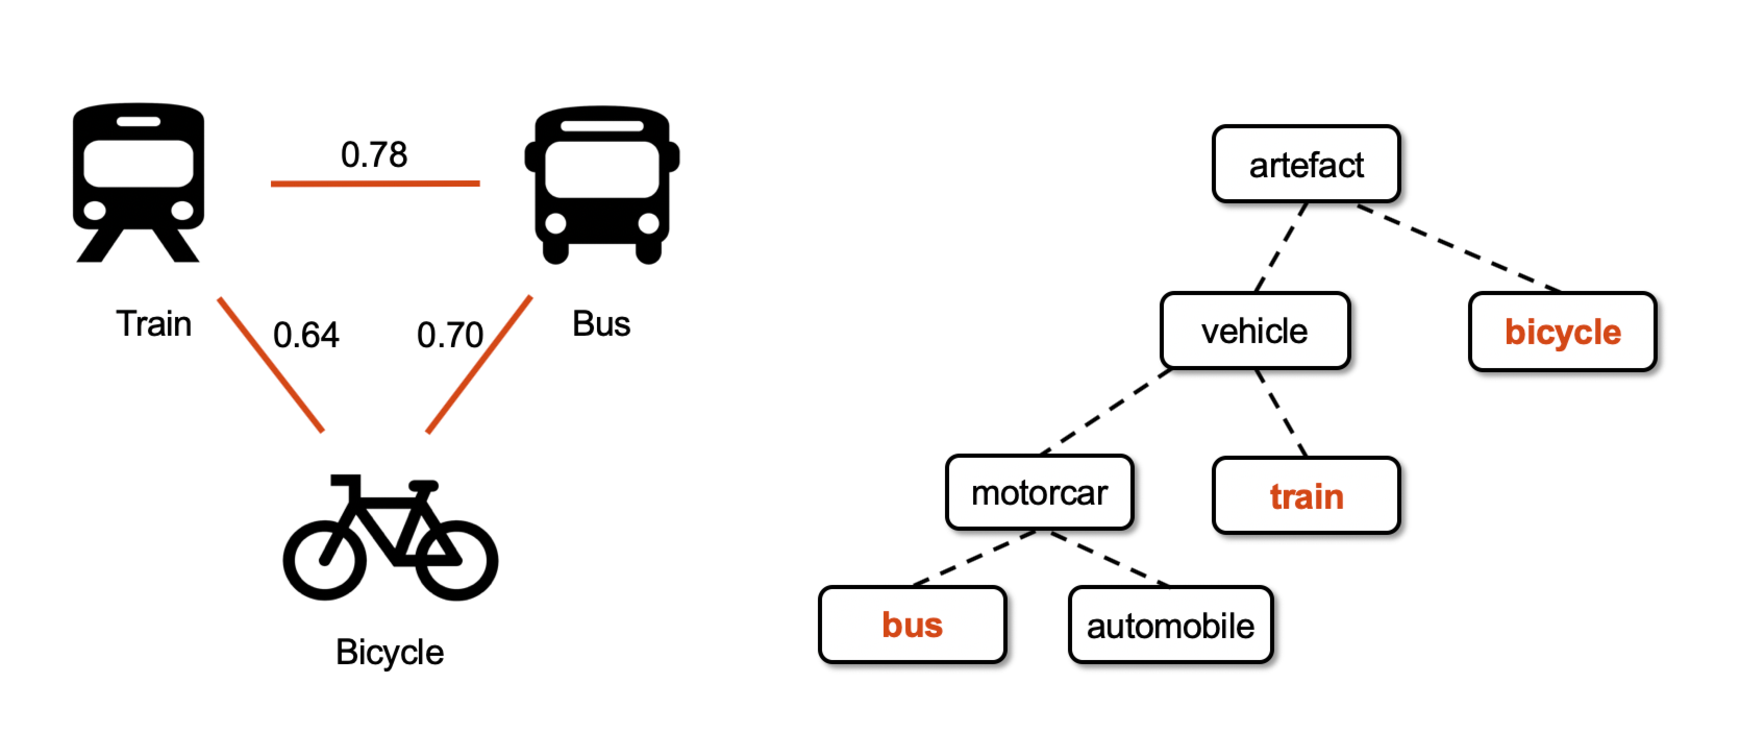
\includegraphics[width=0.9\textwidth]{chap2-1.pdf}}
    \smallcaption{语义关联度与语义相似度区别}
    \label{chap2-1}
\end{figure}

\begin{definition}
    \label{sr}
    {\bf 语义关联度(Semantic Relatedness)}
    对于给定的一对词语$w_1$和$w_2$,他们之间的语义关联度指通过比较$w_1$和$w_2$的语义表征之后,给出的其背后包含的意义或其语义内容之间的相关程度。这种相关程度的度量不仅仅要考虑其含义之间的种属关系,也要考虑其含义之间的其他复杂语义联系,比如部分整体关系、反义关系甚至一些无法准确描述的潜在语义关系。
\end{definition}

\begin{definition}
    \label{ss}
    {\bf 语义相似度(Semantic Similarity)}
    对于给定的一对词语$w_1$和$w_2$,他们之间的语义相似度指通过比较$w_1$和$w_2$在词法库或其隐藏在其他知识库中实体之间的种属关系之后给出的数值评分。相比于语义关联度,语义相似度考虑的词语间关系更加明确。
\end{definition}

\subsection{知识关联网络}
本节利用词语背后隐含的语义内容以及词语之间的共现关系来构建知识关联网络,并用来计算语义关联度。有了清晰的词语间语义关联度的概念之后,本节接下来阐述知识关联网络的相关概念。知识关联网络的构建依赖于知识库的选择,在第\ref{chap:chap01}章中给出的结构化知识库中,如本体库、知识图谱等,其中数据往往以RDF三元组的形式给出,其中三元组和RDF分别指:

\begin{definition}
    \label{rdf}
    {\bf 资源描述框架(Resource Description Framework,RDF)}
    是由万维网联盟(W3C)\footnote{https://www.w3.org/}提出的一组标记语言的技术规范,以便更为丰富地描述和表达网络资源的内容与结构,形式上表现为三元组。
\end{definition}

\begin{definition}
    \label{triple}
    {\bf 三元组(Triple)}
    是描述客观事物或抽象概念的一种方式,形式上表现为主语-谓语-宾语(Subject-Predicate-Object,SPO)。其中主语与宾语分别表示实体对象,而谓语表示连接主语与宾语的关系属性或类别。举个例子来说,\emph{\underline{Bus}(Subject) \underline{is a}(Predicate) \underline{vehicle}(Object)}或者\emph{\underline{Apple company}(Subject) \underline{produces}(Predicate) \underline{iPad}(Object)}。
\end{definition}

但是,对于一类对象以及这类对象的所属属性,RDF作为一种基础数据模型,表达能力有所不足,举个例子来说:\emph{“Yaoming is a basketball player”}和\emph{“Yaoming was born in Shanghai”},对于这样两条事实,RDF可以清晰的定义。但是对于定义\emph{“Yaoming is a person”},\emph{“Shanghai is a city”}以及\emph{person}和\emph{city}这两个对象各自的属性以及他们之间的联系时,不同的研究者会定义不同的属性和联系。为了规范化RDF数据的定义,RDFS(Resource Description Framework Schema)\footnote{https://www.w3.org/TR/rdf-schema/}和OWL(Web Ontology Language)\footnote{https://www.w3.org/OWL/}被提出建立起模式或者原语(Ontology)的概念来定义抽象化实体的属性以及他们之间的联系。

有了以上的这些基础之后,对于以RDF数据模式或其他形式存储的知识库,我们可以通过建立知识库实体与词语之间的联系来构建知识关联网络,这里给出其形式化定义:
\begin{definition}
    \label{kan}
    {\bf 知识关联网络(Knowledge Association Network,KAN)}
    知识关联网络有效地连接起词语与其背后包含的意义之间的联系,其本质上表现为一张图$G=(W, E, R)$,如图\ref{chap1-2}所示,其中$W$为词典中的词语集合,$E$是与$W$中所有词相关联的知识库实体所构成的集合,这样$W$和$E$组成了知识关联网络中的节点集合。而对于边集合$R$, 在KAN中分为三种:词语之间的关系$R_w$、实体之间的关系$R_e$以及词语与实体之间的关系$R_{we}$。
\end{definition}


\section{知识关联网络驱动的语义关联度计算框架}
\label{chap02-sr}
当明确语义关联度与知识关联网络的相关概念之后,本节从整体上介绍如何统筹知识关联网络中边的三种类型来计算最后的关联度值。

\begin{figure}[!ht]
    \centerline{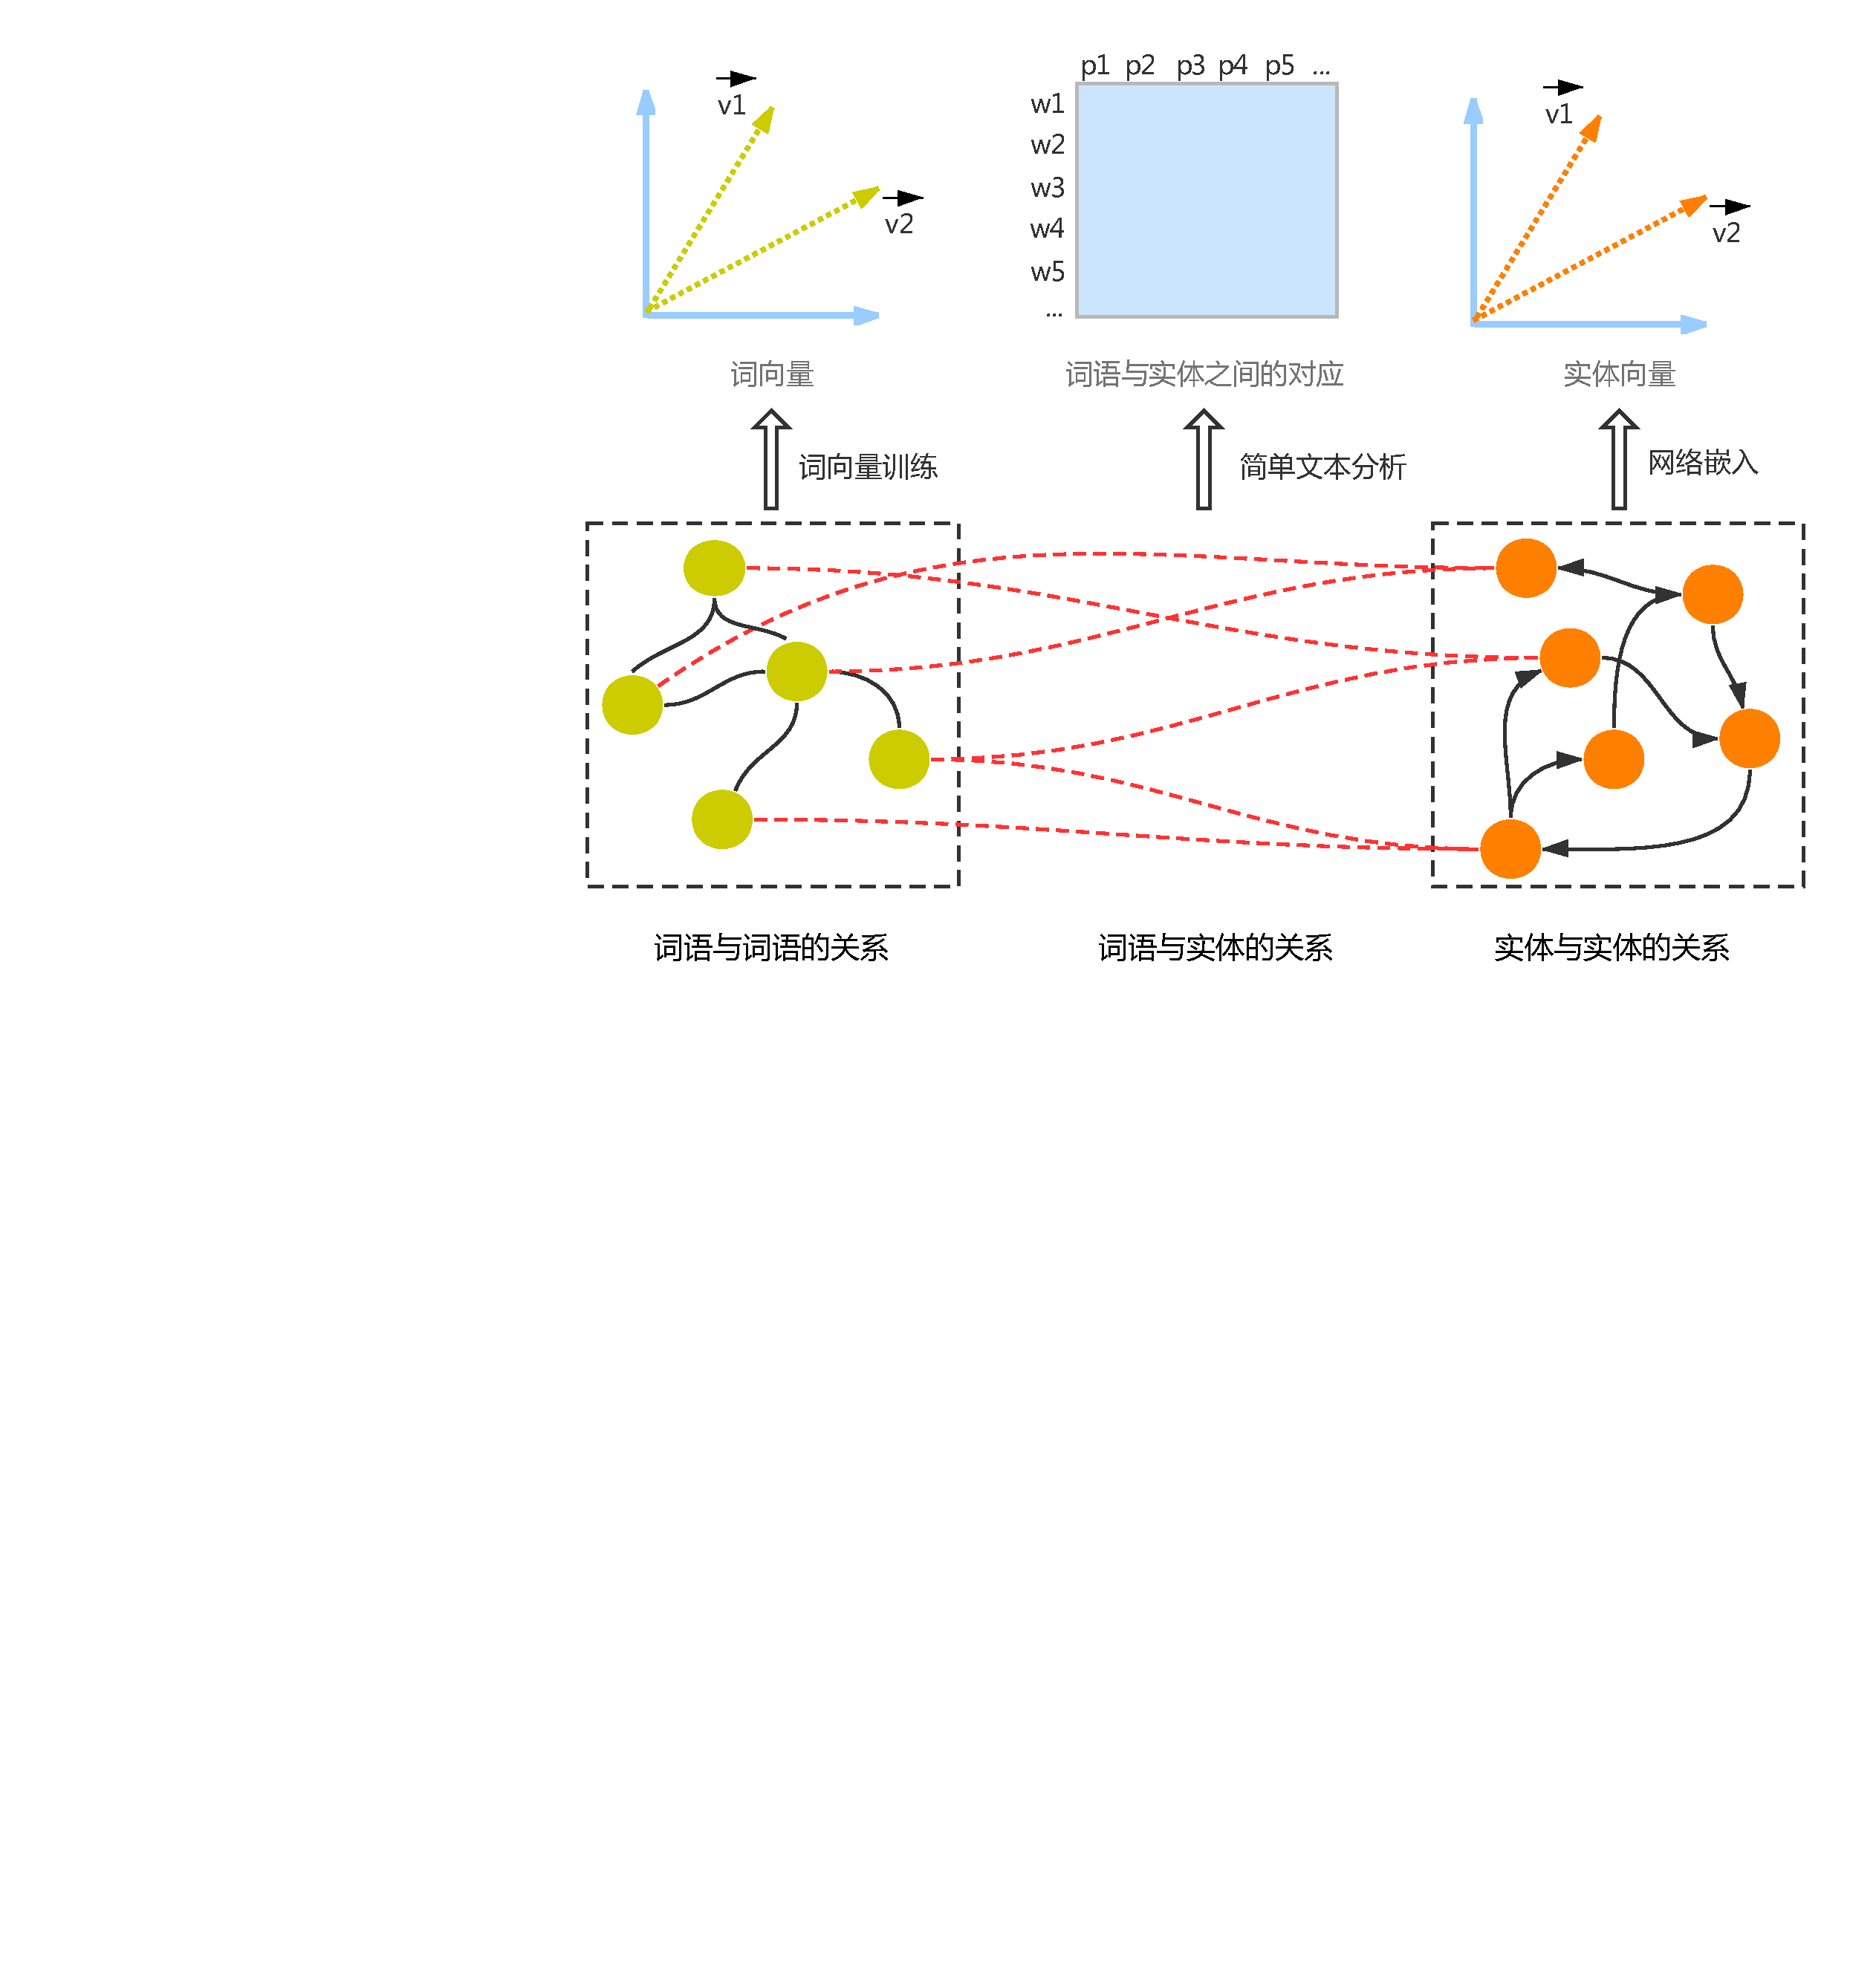
\includegraphics[width=0.9\textwidth]{chap2-2.pdf}}
    \smallcaption{知识关联网络三种边类型对应的处理方法}
    \label{chap2-2}
\end{figure}

如图\ref{chap2-2}所示,对于知识关联网络中的三种关系,我们可以通过不同的方法得到他们之间的数值关联程度。1)词语与词语之间的关系反映了语料库中词语之间的共现关系。这部分我们主要通过词向量训练模型来得到对应的词向量表示,然后通过向量距离计算来得到词语层$w_i$和$w_j$之间的关联度,记为$f_w(w_i, w_j)$;2)词语与实体之间的关系主要起到连接词语层与知识库实体的作用,可以根据词语与实体之间的不同的相关程度得到不同的权重。这部分主要通过文本匹配等简单的处理来建立词语与实体之间的关系,而至于某条关系的权重,记录为$f_{we}(w, e)$,针对不同的知识库选择,关系权重的分配方法不同,本文将在接下来的两章做阐述。3)实体与实体之间的关系反映了词语与实体之间的联系,这部分主要通过不同的网络嵌入模型来学习实体的分布式向量表征,然后实体之间的相似度也可以被快速计算得到,记为$f_{e}(e_i, e_j)$。

当得到知识关联网络中三种关系连接的主体之间的关联度后,本文将最终词语间语义关联度分为两部分:词语层的语义关联度和实体层的语义关联度。对于词语层的语义关联度,本文直接采用词语与词语之间的向量距离作为最终结果,即:
\begin{equation}
F_w(w_i, w_j) = f_{w}(w_i, w_j)
\label{F_w}
\end{equation}


\noindent 对于实体层的语义关联度,本文通过组合词语与实体以及实体与实体之间的关系来计算,如图\ref{chap2-3}所示对于两个词语$i$和$j$,通过其相关实体而连接起两个单词的路径有多条,图中有12条。而对于两个词语$i$和$j$在一条由实体$m$和$n$连通的路径上的关联度,我们可以通过下面的方法得到:
\begin{equation}
    W_{path}(w_i, w_j, e_m, e_n) = f_{we}(w_i, e_m)f_e(e_m, e_n)f_{we}(w_j, e_n)
    \label{wpath}
\end{equation}

\noindent 由此,词语在实体层面的语义关联度可以按照如下公式计算:
\begin{equation}
    F_e(w_i, w_j) = \mathscr{F}_{e_m \in E_i,e_n \in E_j}W_{path}(w_i, w_j, e_m, e_n)
    \label{F_e}
\end{equation}

\begin{figure}[!ht]
    \centerline{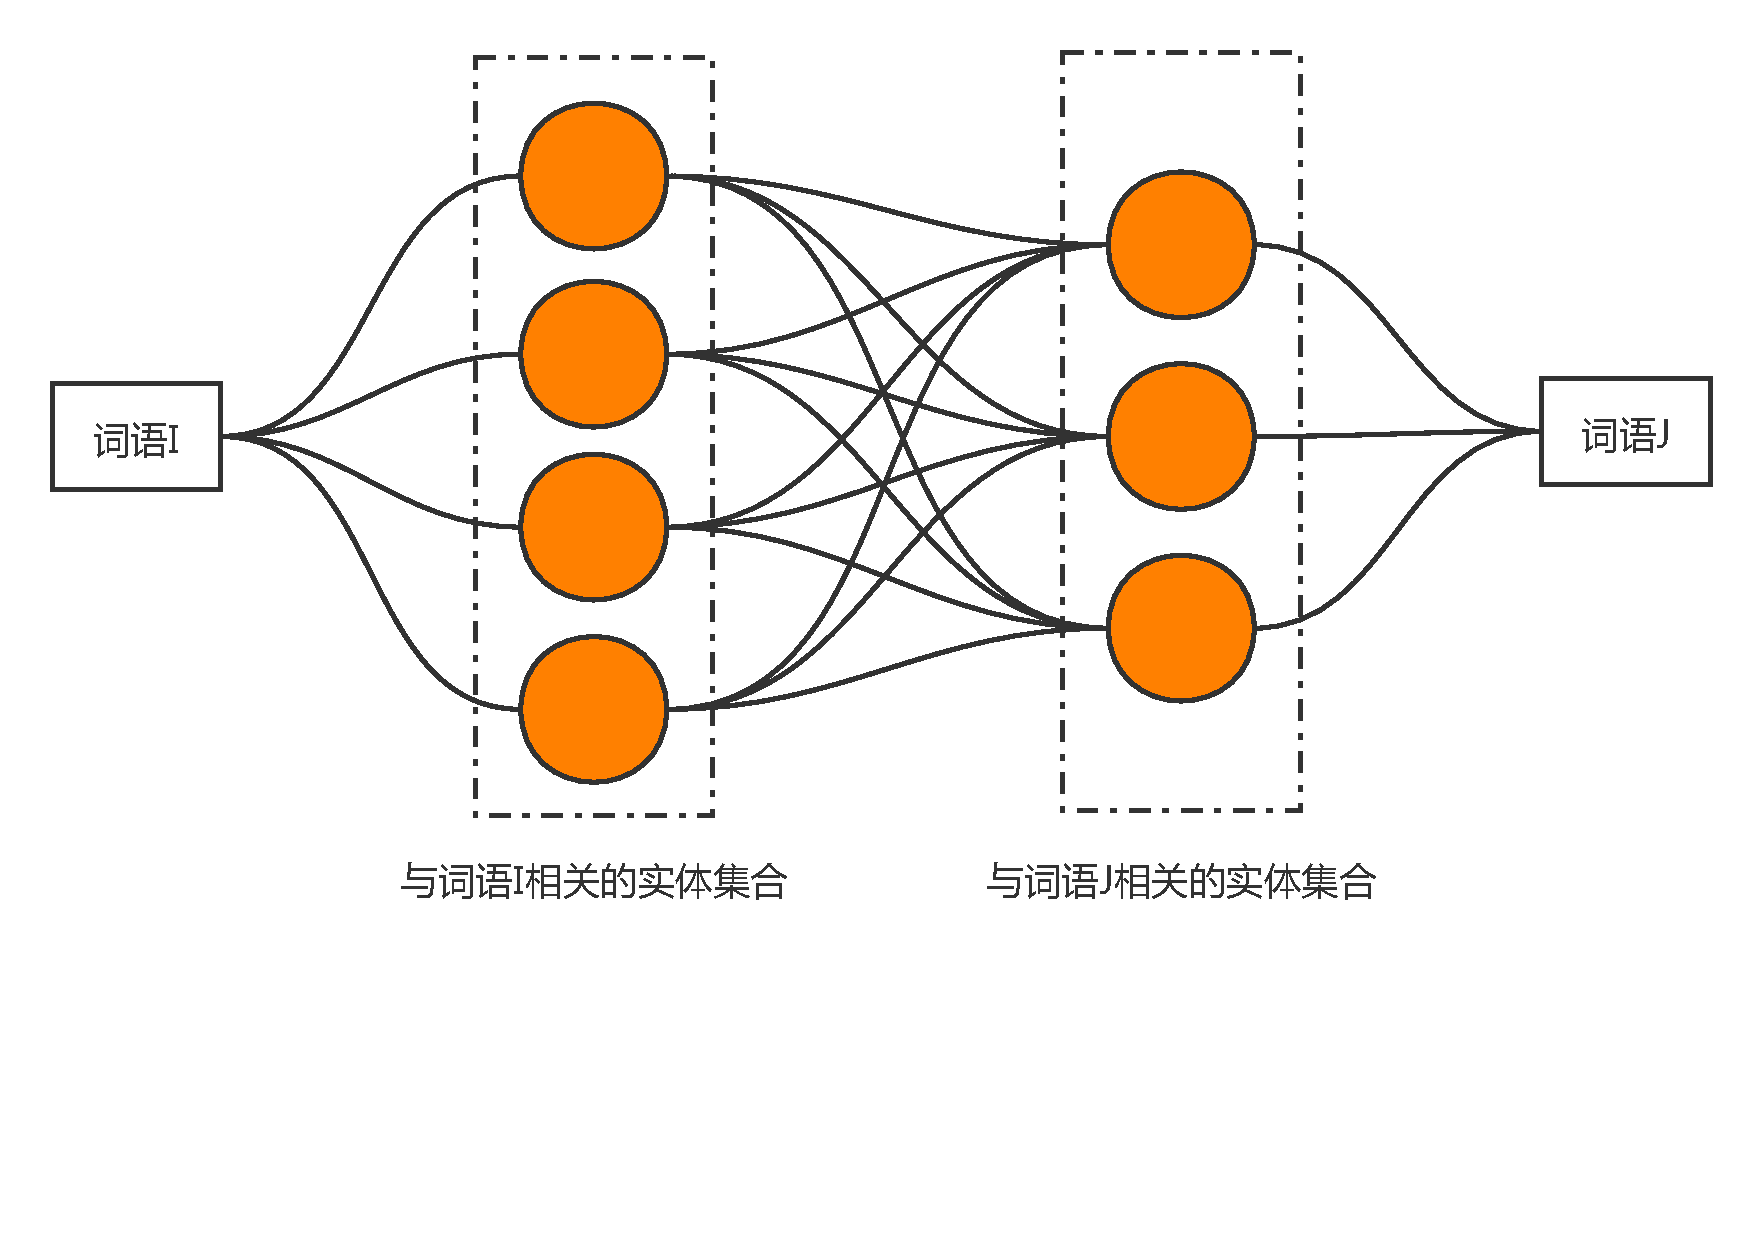
\includegraphics[width=0.8\textwidth]{chap2-3.pdf}}
    \smallcaption{实体层语义关联度度量示例}
    \label{chap2-3}
\end{figure}

\noindent 其中,$E_i$表示与词语$w_i$有连接的所有实体集合,$E_j$类似。而$\mathscr{F}$表示聚合策略,即针对词语之间由相关联实体所构成的多条路径所采用的聚合方法。聚合方法的采用视情况而定,经常采用的的是求平均值的方法,对应公式如下:
\begin{equation}
    F_{e;avg}(w_i, w_j) = \sum_{e_m \in E_i}^{ }\sum_{e_n \in E_j}^{ }W_{path}(w_i, w_j, e_m, e_n)
    \label{F_e_avg}
\end{equation}

\noindent 特殊的,当词语与实体层之间的边权重无法准确衡量时,本文还采用了取实体间关联度最大值的策略来衡量词语在实体层的语义信息:
\begin{equation}
    F_{e;max}(w_i, w_j) = \max_{e_m \in E_i,e_n \in E_j}f_e(e_m, e_n)
    \label{F_e_max}
\end{equation}

\noindent 最后可以得到最终的词语间语义关联度为:
\begin{equation}
    F(w_i, w_j) = \varphi F_w(w_i, w_j) + (1 - \varphi) F_e(w_i, w_j)
    \label{F}
\end{equation}

\noindent 其中$\varphi$取值空间为$[0,1]$,起到了平衡词语层语义关联度$F_w$和实体层语义关联度$F_e$的作用。最后我们给出整个过程的算法流程:

\begin{algorithm}
    \smallcaption{知识关联网络驱动的语义关联度计算流程}
    \label{alg:kan-sr}
    \SetKwInOut{Input}{输入}
    \SetKwInOut{Output}{输出}
    \SetKw{Return}{return}
    \Input{KAN, 词语$w_i$, $w_j$, 预训练好的所有词向量$v_w$, 所有实体向量$v_e$, 词语与实体之间的关联值$f_{we}$, $\varphi$}
    \Output{语义关联度值$F{(w_i,w_j)}$}
    \BlankLine
    查询KAN得到$w_i$和$w_j$的关联实体集合$e(w_i), e(w_j)$ \;
    $F_w(w_i, w_j) \leftarrow f_w(w_i, w_j) \leftarrow cos(\vec v_{wi},\vec v_{wj})$ \;
    \For{$e_m \in e(w_i)$, $e_n \in e(w_j)$} {
        $f_e(e_m, e_n) \leftarrow cos(\vec v_{em},\vec v_{en})$ \;
        $W_{path}(w_i, w_j, e_m, e_n) \leftarrow f_{we}(w_i, e_m)f_e(e_m, e_n)f_{we}(w_j, e_n)$; \;
    }
    $F_e(w_i, w_j) \leftarrow \mathscr{F}_{e_m \in E_i,e_n \in E_j}W_{path}(w_i, w_j, e_m, e_n)$ \;
    $F(w_i, w_j) \leftarrow \varphi F_w(w_i, w_j) + (1 - \varphi) F_e(w_i, w_j)$ \;
    \Return $F(w_i, w_j)$
\end{algorithm}


\section{本章小结}
本章首先通过一个简单的例子阐述了语义关联度和语义相似度的区别并给出了定义,随后对知识库的主要数据存储模式RDF做了简要阐述。有了这些基础之后,本章还介绍了如何组合知识关联网络中三种关系来计算最终的语义关联度,并给出了算法流程。

  % \chapter[基于WordNet构建的知识关联网络驱动的语义关联度计算]{\texorpdfstring{基于WordNet构建的知识关联网络驱动 \protect\\ 的语义关联度计算}{基于WordNet构建的知识关联网络驱动的语义关联度计算}}
\chapter{基于WordNet的语义关联度模型}
\label{chap:chap03}
本章采用WordNet作为构建知识关联网络的知识库,并采用更具表达能力的分布式向量来表征实体语义信息,由此利用WordNet中实体的语义信息来丰富词语间的语义关联度度量。

\section{WordNet简介}
%选用WordNet的理由
\begin{figure}[!ht]
    \centerline{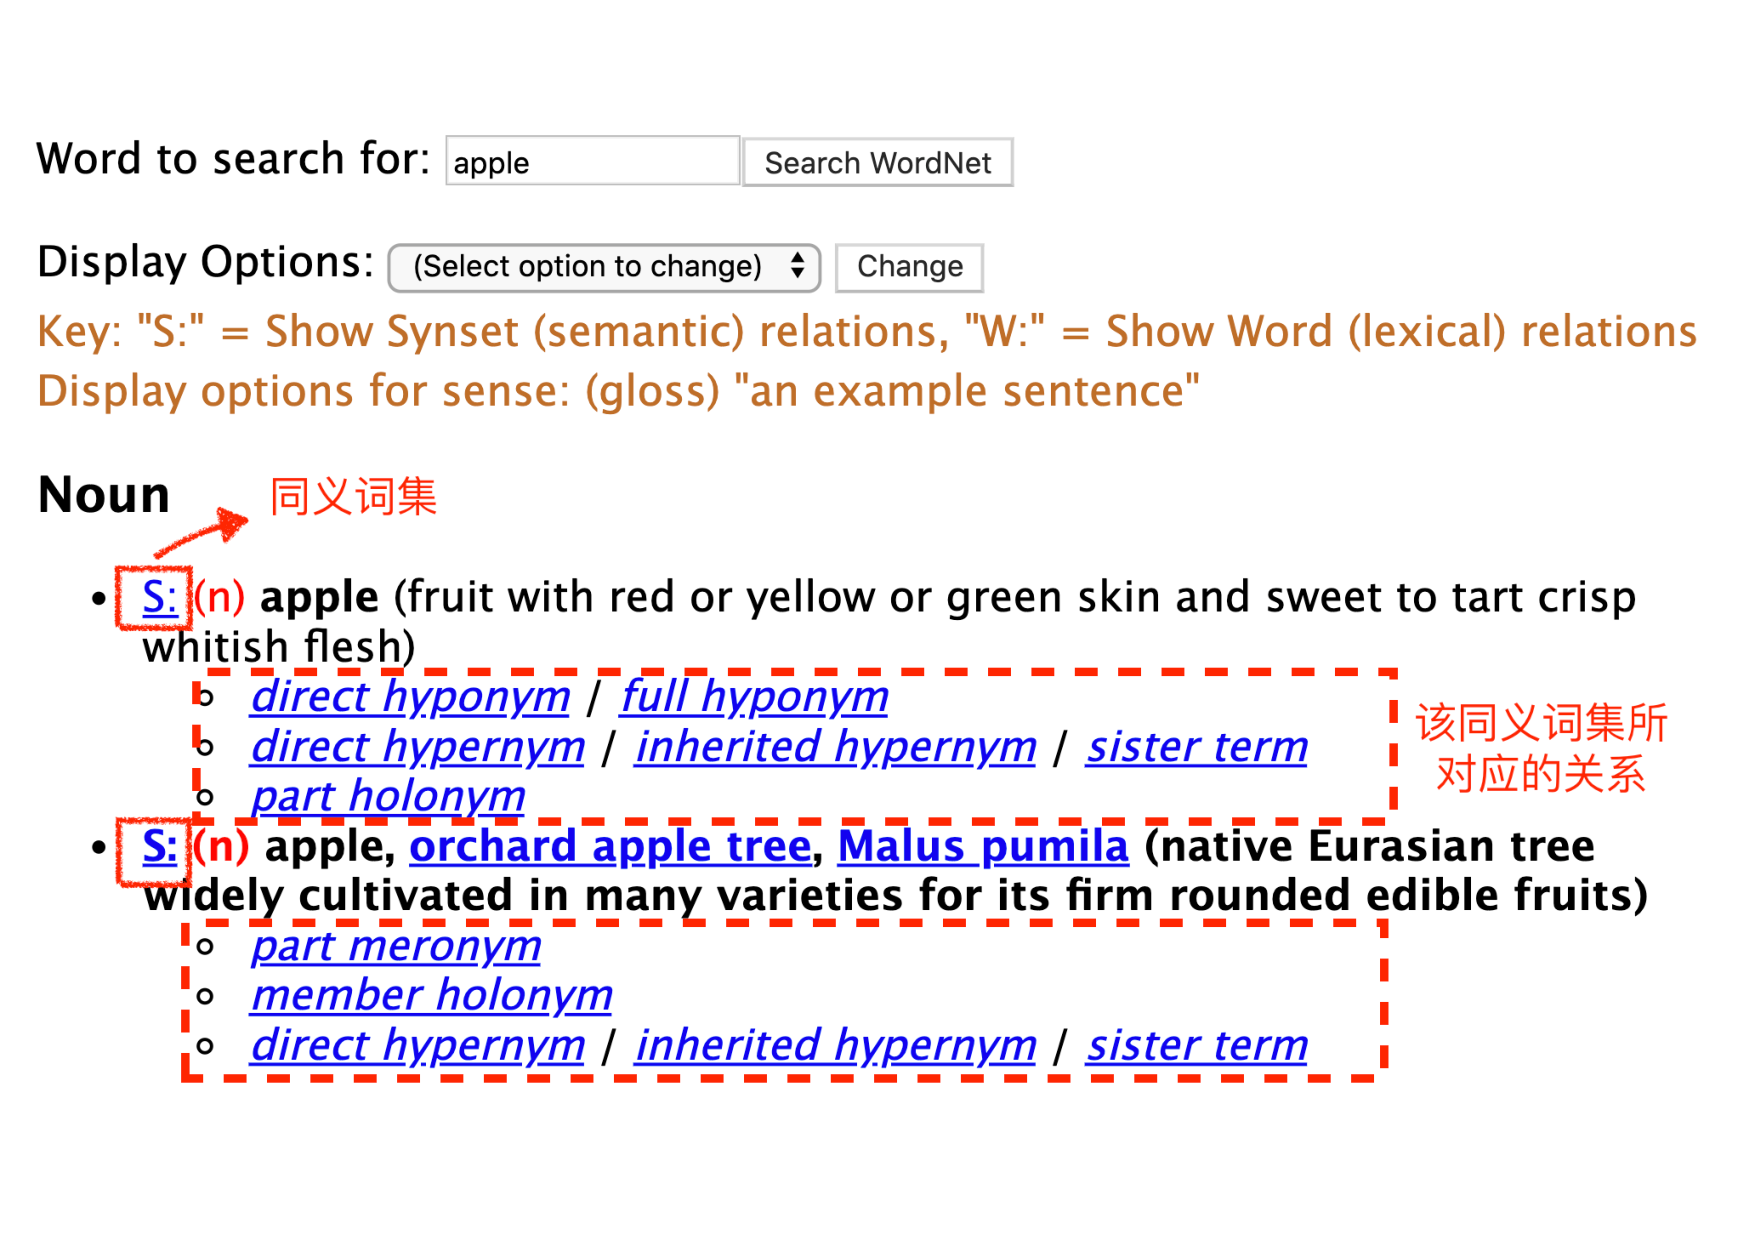
\includegraphics[width=0.8\textwidth]{chap3-1.pdf}}
    \smallcaption{WordNet同义词集示例}
    \label{chap3-1}
\end{figure}

WordNet作为一种英文词法关系库,其按照单词(主要包含名词、动词、形容词和副词)之间的语义内容和词法关系,由专家与计算机合作将大量英文单词划分为一组组同义词集。这种按照意义分组的创建方式使得WordNet即不局限于传统词法词典,也不同于同义词词林,WordNet不仅仅是用同义词集的方式去展示客观概念或主观事物,同义词集之间更由不同语义关系相关联着,这些关系有上下位关系(hyponymy)、整体部分关系(meronymy)、继承关系(entailment)等。如图\ref{chap3-1}所示,对于单词\emph{apple},WordNet中有两个实体与之对应,这两个实体分别描述了\emph{apple}作为一种水果的意义和作为一种植物的意义,同时这两个实体又分别有自己的关系属性,连接了其他与之关联的实体。

传统研究者\cite{its/Rada89, Leacock98, wu1994verb, tkde/LiBM03}主要利用WordNet中同义词集的距离信息来衡量词语之间的语义差别,这种方法多用来建模词语间的层次关系,在语义相似度方面表现较好,但是对于涉及多种语义关系的关联度度量,这种方法表现不太好。为了弥补这些缺点,本文通过网络嵌入的方式学习到更具表达能力的分布式向量表示,由此来更好的完成语义关联度度量。

%构建
\section{知识关联网络构建}
对于知识关联网络的构建,首先要解决的问题是建立起词语与实体之间的直接联系。幸运的是,WordNet中提供了相应的查询接口来得到与词语相关的实体,其中最常用的接口是由宾夕法尼亚大学提出的自然语言处理工具包NLTK(Natural Language Toolkit)\cite{OM/Bird09}。NLTK中针对超过50种自然语言处理领域常用的语料和词法数据库提出了简单易上手的访问接口,在针对WordNet的接口中\footnote{https://www.nltk.org/howto/wordnet.html},对于给定的单词,研究者们可以方便查询到与之相关的实体,反之对于给定的实体,也可以查询到与其相关联的多个单词。在知识关联网络的实体层,本文主要考察了WordNet中的上位关系(hypernyms)、下位关系(hyponyms)以及部分整体关系(member holonyms)。

\section{语义关联度计算}
当词语与实体之间的联系被建立后,相应的语义关联度计算主要分为三部分:词语与词语之间的关联度、实体与实体之间的关联度以及词语与实体之间的关联度度量。本节将对这三个部分做详细介绍。

\subsection{词语之间的语义关联度计算}
\label{word2vec}
词语层面的语义关联度计算主要包含两类方法:1)Word2Vec~\cite{corr/Mikolov13}和GloVe~\cite{emnlp/PenningtonSM14}等在大规模高质量语料库上训练的分布式向量表征方法;2)基于词语间共现原则的方法~\cite{aaai/StrubeP06, ijcai/GabrilovichM07}。以往的实验已经证明,前者训练得到的分布式向量表示可以更好地捕捉到词语的潜在语义信息,相比于基于共现原则的方法效果更好。因此本文采用Word2Vec的方法去训练Wikipedia来得到词向量。对于两个词语$w_i$和$w_j$来说,训练得到的词向量分别记为$\vec v_i$和$\vec v_j$,则$w_i$和$w_j$在词语之间的语义关联度$f_w(w_i, w_j)$可以通过向量余弦运算得到,有:
\begin{equation}
    \label{cos}
    f_w(w_i, w_j) = cos(\vec v_i,\vec v_j) = \frac{\vec v_i \cdot 
    \vec v_j}{\left \| \vec v_i \right \|\left \| \vec v_j \right \|}
\end{equation}

值得注意的是Word2Vec中包含有两种不同的模型来训练词向量,他们分别是SkipGram和连续词袋模型(Continuous bag-of-words, CBOW),SkipGram模型训练过程主要是利用当前词来预测其邻居词,而CBOW模型则相反是利用邻居词预测当前词。两种方法各有利弊,假设当前词典大小为N,窗口设定大小为K,对于SkipGram模型,由于要对窗口内所有词做预测,其预测过程将是CBOW模型的K倍。而CBOW模型由于利用了所有邻居词来预测当前词,低频词被预测的次数就会变少,因此对于低频词来说CBOW模型表现往往不太好。此外为了加速模型训练过程,Word2Vec中还提出了两种处理方法,分别是层次Softmax(Hierarchical Softmax)和负采样策略(Negative Sampling)。具体这里本文不详细展开,更多的参数设置将在第\ref{chap:chap05}章实验部分介绍。

\subsection{词语与实体之间的的语义关联度计算}
WordNet中虽然按照词语的不同含义存储着词语与实体之间构成的多对多关系,但是词语与实体的关联程度值无法被得到。为了得到词语与其含义对应的实体之间的关联程度值,一般思路会将语料库中的自然语言表述与WordNet实体建立对应,然后统计不同表述的频率来为不同实体分配权重。然而将自然语言表述与WordNet实体建立对应的过程属于实体链接的范畴(Entity Linking)~\cite{luwei},链接过程本身就有信息损耗。因此,对于基于WordNet构建知识关联网络中的词语与实体之间关系,本章不做考虑,即认为词语与其每个相关联的实体都是等权重联系的。

\subsection{实体之间的语义关联度计算}

\textbf{注意力机制:}
本文的目标是得到实体关系图中每个实体的分布式向量表示,由此较好地保留实体的语义信息。实体之间的联系本质上表现为一张图,其中一个实体的语义表征受其周围实体的影响,而且不同邻居实体对其语义表征的贡献度也不一样。近年来提出的注意力机制可以在一定程度上解决这种问题,学习到不同邻居节点与中心节点之间的的关联权重。在本节中,给定相连实体$i$和实体$j$,对于其初始输入向量表征$\vec h_i$和$\vec h_j$,本文定义为其所关联的单词词向量平均值,然后采用自注意力(self-attention)~\cite{corr/VaswaniSPUJGKP17, iclr/VelickovicCCRLB18}机制来学习他们之间的权重$e_{ij}$,有:
\begin{equation}
    e_{ij} = LeakyRelu\big(\vec a^T[W\vec h_i || W\vec h_j]\big)
    \label{gat_e_ij}
\end{equation}
\noindent 其中,$\parallel$表示矩阵拼接操作,$\cdot^T$表示矩阵转置操作。$W$作为初始化的线性矩阵,主要起到对网络输入做线性变换的作用,此处$a$作为权重矩阵与后面紧跟的$LeakyRelu$激活层构成简单的前馈神经网络,来学习邻居节点的权重分布。之后,为了统一各个节点之间的权重范围,本文通过$softmax$函数来将其归一化:
\begin{equation}
    \alpha_{ij} = softmax(e_{ij}) = \frac{exp(e_{ij})}{\sum_{k\in N_i}exp(e_{ik})}
    \label{alpha_ij}
\end{equation}
\noindent 其中$N_i$是由节点$i$和其邻居节点构成来的节点集合。到这里一个节点与其周围节点的权重分布可以被得到,本文通过加权求和的方式得到当前节点的新表征,然后将其输入激活函数$Elu$得到$\vec h_i^{'}$:
\begin{equation}
    \vec h_i^{'} = Elu\Bigg(\sum_{j \in N_i}{\alpha_{ij} W\vec h_j}\Bigg)
    \label{h_i_t}
\end{equation}

为了模型能够捕捉更多的节点语义空间,同时使得训练过程更稳定,本文采用多头注意力机制(multi-head attention)~\cite{corr/VaswaniSPUJGKP17}来增加模型鲁棒性。具体来说,本文重复上面的self-attention过程K次,然后对这K次产生的$\vec h_i^{'}$进行拼接:
\begin{equation}
    \vec h_i^{'} = Elu\Bigg(\mathop{\parallel}\limits_{k=1}^{K} \Bigg(\sum_{j \in N_i}{\alpha_{ij}^{k} W^k\vec h_j}\Bigg)\Bigg)
    \label{k_heads_1}
\end{equation}
\noindent 其中,$\parallel$表示矩阵拼接操作,$\alpha_{ij}^{k}$表示第k次self-attention学习到的节点$i$和节点$j$的边权重。值得注意的是,当使用多注意力机制学习的结果直接作为输出时,往往采用平均策略去适应模型的输出维数,有:
\begin{equation}
    \vec h_i^{'} = Elu\Bigg(\frac{1}{K}\sum_{k=1}^{K}\sum_{j \in N_i}{\alpha_{ij}^{k} W^k\vec h_j}\Bigg)
    \label{k_heads_2}
\end{equation}


\textbf{模型与目标函数:}
在语义关联度计算任务中,本文采用两层上文提到的注意力模型来学习网络实体向量表示。如算法\ref{alg:self-att}第一行所示,在第一层输入部分本文取跟实体$e_i$相关联的所有词语的词向量$\vec v_{wm}$的平均值来作为输入替代随机初始化,multi-head注意力机制部分,本文采用拼接的方法得到新的实体向量表示,并作为下层的输入,最后的网络输出则采用平均策略输出。

学习WordNet中实体的向量表示是一个无监督的任务。在网络嵌入中模型的训练往往基于这样一个假设:互为邻居的节点语义空间相近,其在向量空间得到的嵌入表示距离也相近,而对于不相连的节点,他们在向量空间得到的嵌入表示距离更远。基于此,本文采用二分类交叉熵损失函数(Binary Cross Entropy Loss,BCE)作为目标函数,将图中存在的边作为正例,然后通过负采样的方法得到负例边,损失函数如下:
\begin{equation}
    \mathcal{L} = -\sum_{i = 0}^{N} [y^{(i)} \times log\sigma(\vec h^{(i)} \times \vec t^{(i)})+(1 - y_{}^{(i)})\times log\sigma(1 - \vec h^{(i)} \times \vec t^{(i)}))]
    \label{wordnet_loss}
\end{equation}

\noindent 其中$N$为正负例边的总数,$\vec h^{(i)}$和$\vec t^{(i)}$分别表示连接第$i$条边的两个节点的网络输出向量表示,头节点$\vec h^{(i)}$和尾节点$\vec t^{(i)}$。$y^{(i)}$为正负例边标签,正例为1,负例为0。模型优化器方面,本文采用自适应调整学习率的Adam(Adaptive Moment Estimation)算法来优化目标函数,由此得到实体向量表示。

\begin{algorithm}
    \smallcaption{自注意力网络无监督嵌入流程}
    \label{alg:self-att}
    \SetKwInOut{Input}{输入}
    \SetKwInOut{Output}{输出}
    \SetKw{Return}{return}
    \Input{KAN, 输入向量权重矩阵$W$,$a$}
    \Output{网络节点向量表示$\vec h^{'}$}
    $h_i \leftarrow mean(\sum_{m \in rel(e_i)} \vec v_{wm})$ \;
    \For{i = 1 to 2}{
        \For {k = 1 to K} {
            $\alpha_{ij}^k \leftarrow \frac{exp(LeakyRelu\big(\vec a^T[W^k\vec h_i || W^k\vec h_j]\big))}{\sum_{k\in N_i}exp(LeakyRelu\big(\vec a^T[W^k\vec h_i || W^k\vec h_k]\big))}$ \;
            \If {i == 1} {
                $\vec h_i^{'} \leftarrow \vec h_i^{'} \parallel Elu\Bigg(\sum_{j \in N_i}{\alpha_{ij}^{k} W^k\vec h_j}\Bigg)$ \;
            } \Else {
                $\vec h_i^{'} \leftarrow \vec h_i^{'} + \sum_{j \in N_i}{\alpha_{ij}^{k} W^k\vec h_j}$ \;
            }
        }
    }
    $\vec h_i^{'} \leftarrow Elu(\frac{h_i^{'}}{K})$
\end{algorithm}

\subsection{语义关联度计算}
当得到词语与词语、词语与实体以及实体与实体之间的关联后,本文按照章节\ref{chap02-sr}中所述的语义关联度计算框架来计算语义关联度。由于在本部分,词语与实体之间的关联度权重不易获得,所以在组合词语与实体以及实体与实体之间的关系去得到词语在实体层的关联度部分,本文分别采用了基于取平均值和取最大值的策略,其中对于取平均值策略,对公式\ref{F_e_avg}简化得到:
\begin{equation}
    F_{e;avg}(w_i, w_j) = mean(\sum_{e_m \in E_i}^{ }\sum_{e_n \in E_j}^{ }f_e(e_m, e_n))
    \label{F_e_avg_simple}
\end{equation}
\noindent 然后将其带入公式\ref{F},即可得到最后的词语间关联度值。


\section{本章小结}
本章首先对WordNet进行了简要的介绍,并抽取出WordNet中的多种实体关系来构建知识关联网络。之后,对于实体层的网络结构,本文采用更具表达能力的图注意力网络机制来学词实体的分布式向量表示,由此利用词语在WordNet中关联实体的语义信息来丰富词语间的语义关联度度量。
  \chapter{基于DBpedia的语义关联度模型}
\label{chap:chap04}

在本章节,我们基于DBpedia构建知识关联网络,对于其中词语与实体之间的对应关系,本文综合考虑文本外链与文章对词语的影响来计算词语与实体的关联度。在实体层,我们提出一种实体嵌入方法,综合考虑实体周围的属性信息及其所处的网络结构的拓扑信息。由此,我们可以更好地利用实体之间的语义信息计算词语之间的语义关联度。

\section{DBpedia简介}

\begin{figure}[!ht]
    \centerline{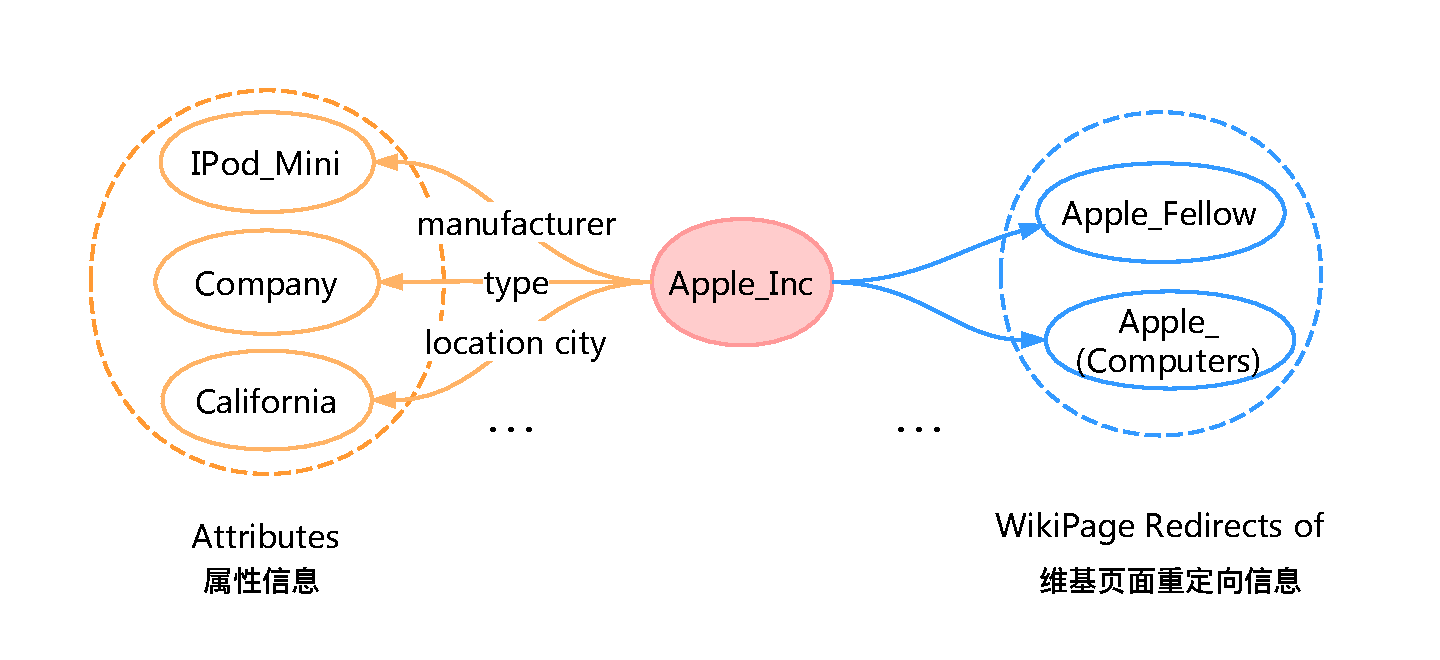
\includegraphics[width=0.9\textwidth]{chap4-1.pdf}}
    \smallcaption{DBpedia中实体的语义特征示例}
    \label{chap4-1}
\end{figure}

% 意义
DBpedia是一项由开源社区维护的百科开源知识图谱,它源自于Wikipedia又不止与此。基于万物互连的思想,DBpedia连接起了Wikipedia、Wikitionary、WordNet以及其它大型开源知识库如Yago等,不仅如此,DBpedia还提供了可供全网访问的服务,研究者们可以以DBpedia为基础挖掘到越来越多的知识信息,大大方便了各项人工智能任务的推进。

至2016年10月,DBpedia中包含了大约600万实体和13亿条RDF三元组,实体周围包含着丰富的语义信息。如图\ref{chap4-1}所示,对于科技公司\emph{Apple},其在DBpedia中有唯一的URI(统一资源定位符)表示\emph{<http://dbpedia.org/page/Apple\_Inc>},简记为\emph{Apple\_Inc},同时还有多种实体以不同关系与\emph{Apple\_Inc}相连。其中,如\emph{Apple\_Inc}是\emph{IPod\_Mini}的生产商、\emph{Apple\_Inc}是一家公司\emph{Company}以及\emph{Apple\_Inc}位于\emph{California}等等描述了该实体的属性(Attributes)空间;而另一些关系如图\ref{chap4-1}所示,不包含明确的语义信息,仅仅在语料库中与该实体通过页面重定向关系(Wikipage Redirects of)相连。

%存储
DBpedia中实体及其边的关系主要以RDF的形式存储在开源图数据库OpenLink Virtuoso\footnote{https://virtuoso.openlinksw.com/}中,并且用户可以通过Virtuoso开放的SPARQL端口\footnote{http://dbpedia.org/sparql}来通过HTTP请求访问DBpedia中的数据。其中SPARQL是一种针对RDF数据的图查询语言,能够自定模式来查询知识图谱中符合模式条件的三元组。


\section{知识关联网络构建}

\begin{figure}[!ht]
    \centerline{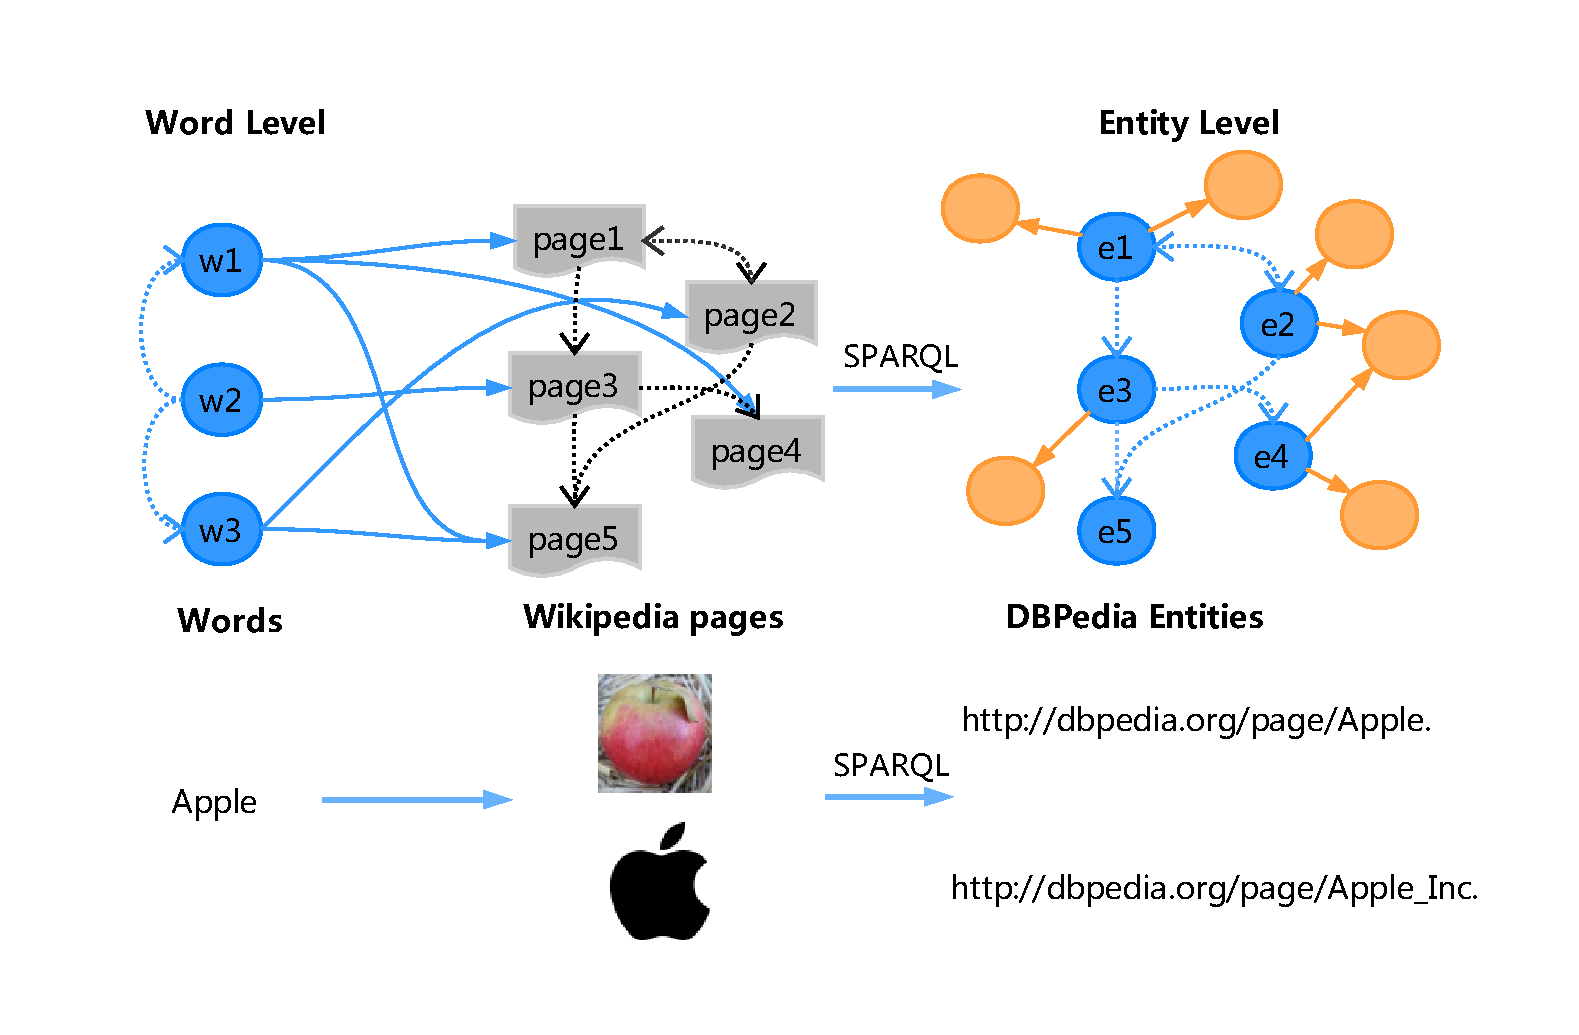
\includegraphics[width=1\textwidth]{chap4-2.pdf}}
    \smallcaption{基于DBpedia中构建的知识关联网络示例}
    \label{chap4-2}
\end{figure}

在上一章中基于WordNet构建的知识关联网络中,词语与WordNet实体之间的对应关系被人工标记并存储在WordNet中,可以很方便地被查询到。与之不同的是,我们无法直接拿到词语与DBpedia实体的关系。但是语料库Wikipedia中则包含了丰富的词语,其文本由词语构成,分类信息、外链信息等也都自然地表现为文本。而且Wikipedia中的页面也与DBpedia中的实体一一对应。文本基于这种对应关系,通过Wikipedia建立其词语与DBpedia中实体的对应关系。

如图\ref{chap4-2}所示,我们给出了基于DBpedia构建知识关联网络的例子。对于一个给定的单词$apple$,通过TF-IDF或词频统计等文本分析手段,我们可以得到与之相关的维基页面,比如维基百科中描述一种水果的$Apple$页面和描述一家公司的$Apple\_Inc$页面,其中每个维基页面有一个重要的属性叫做\emph{WikiPageId},形式上表现为数字,唯一地标示了Wikipedia中的一篇文章。这个属性在DBpedia中也作为对应实体的属性存在。因此我们可以通过SPARQL查询到对应的DBpedia实体。举个例子来说,描述一种水果的$Apple$页面的\emph{WikiPageId}的值是$856$,我们可以通过如下的查询语言得到对应的DBpedia实体。

\begin{lstlisting}[basicstyle=\fontsize{10}{11}\ttfamily,aboveskip=1em,frame=shadowbox]
    PREFIX dbo: <http://dbpedia.org/ontology/>
    SELECT ?E WHERE {
        ?E dbo:wikiPageID 856.
    }
\end{lstlisting}

对于DBpedia中实体周围的语义信息,本文将其分为属性信息(图\ref{chap4-2}中橘色节点所示)和拓扑结构信息,其中属性信息如上节中图\ref{chap4-1}所示明确地描述了实体的属性,而拓扑结构信息反映了实体之间的结构信息。在本文中为了更方便地表示实体的属性与拓扑结构空间,我们将实体属性所构成的图表示为$G_{attr} = \{a_1, a_2, ..., a_n\}$, 其中每个$a_i$描述了一条关系,这段关系以三元组的形式表现,由头实体(h)、关系(r)和尾实体(t)构成,即$a_i = (h, r, t)$。而对于实体所处的拓扑结构,我们将其定义为$G_{t} = (E, R_{redirect})$,表示由边$R_{redirect}$即\emph{WikiPageRedirectOf}连接的所有实体集$E$所构成的图。由此我们可以应用网络嵌入模型来学习实体的属性空间与拓扑结构空间的向量表示。

\section{语义关联度计算}
如图\ref{chap4-3}所示,我们给出了基于DBpedia中构建的知识关联网络驱动的语义关联度计算流程,图中实线表示了模型的处理流程,而虚线表示了一种将输入部分转化为输出部分的处理方法。可见我们的模型主要包含下面三个部分:1)经过对Wikipedia的简单预处理,我们得到词语与维基百科页面的对应关系;2)由维基页面唯一的\emph{id},经过SPARQL查询得到维基页面对应的DBPedia实体,连接起词语与实体的对应关系;3)对于知识关联网络实体层的语义信息,我们将其分为属性空间与拓扑结构空间,并采用不同的网络嵌入模型去得到实体的向量表示。最后,我们综合考虑词语与词语、词语与实体以及实体与实体之间的语义关联度去构成最后的关联度度量。

\begin{figure}[!ht]
    \centerline{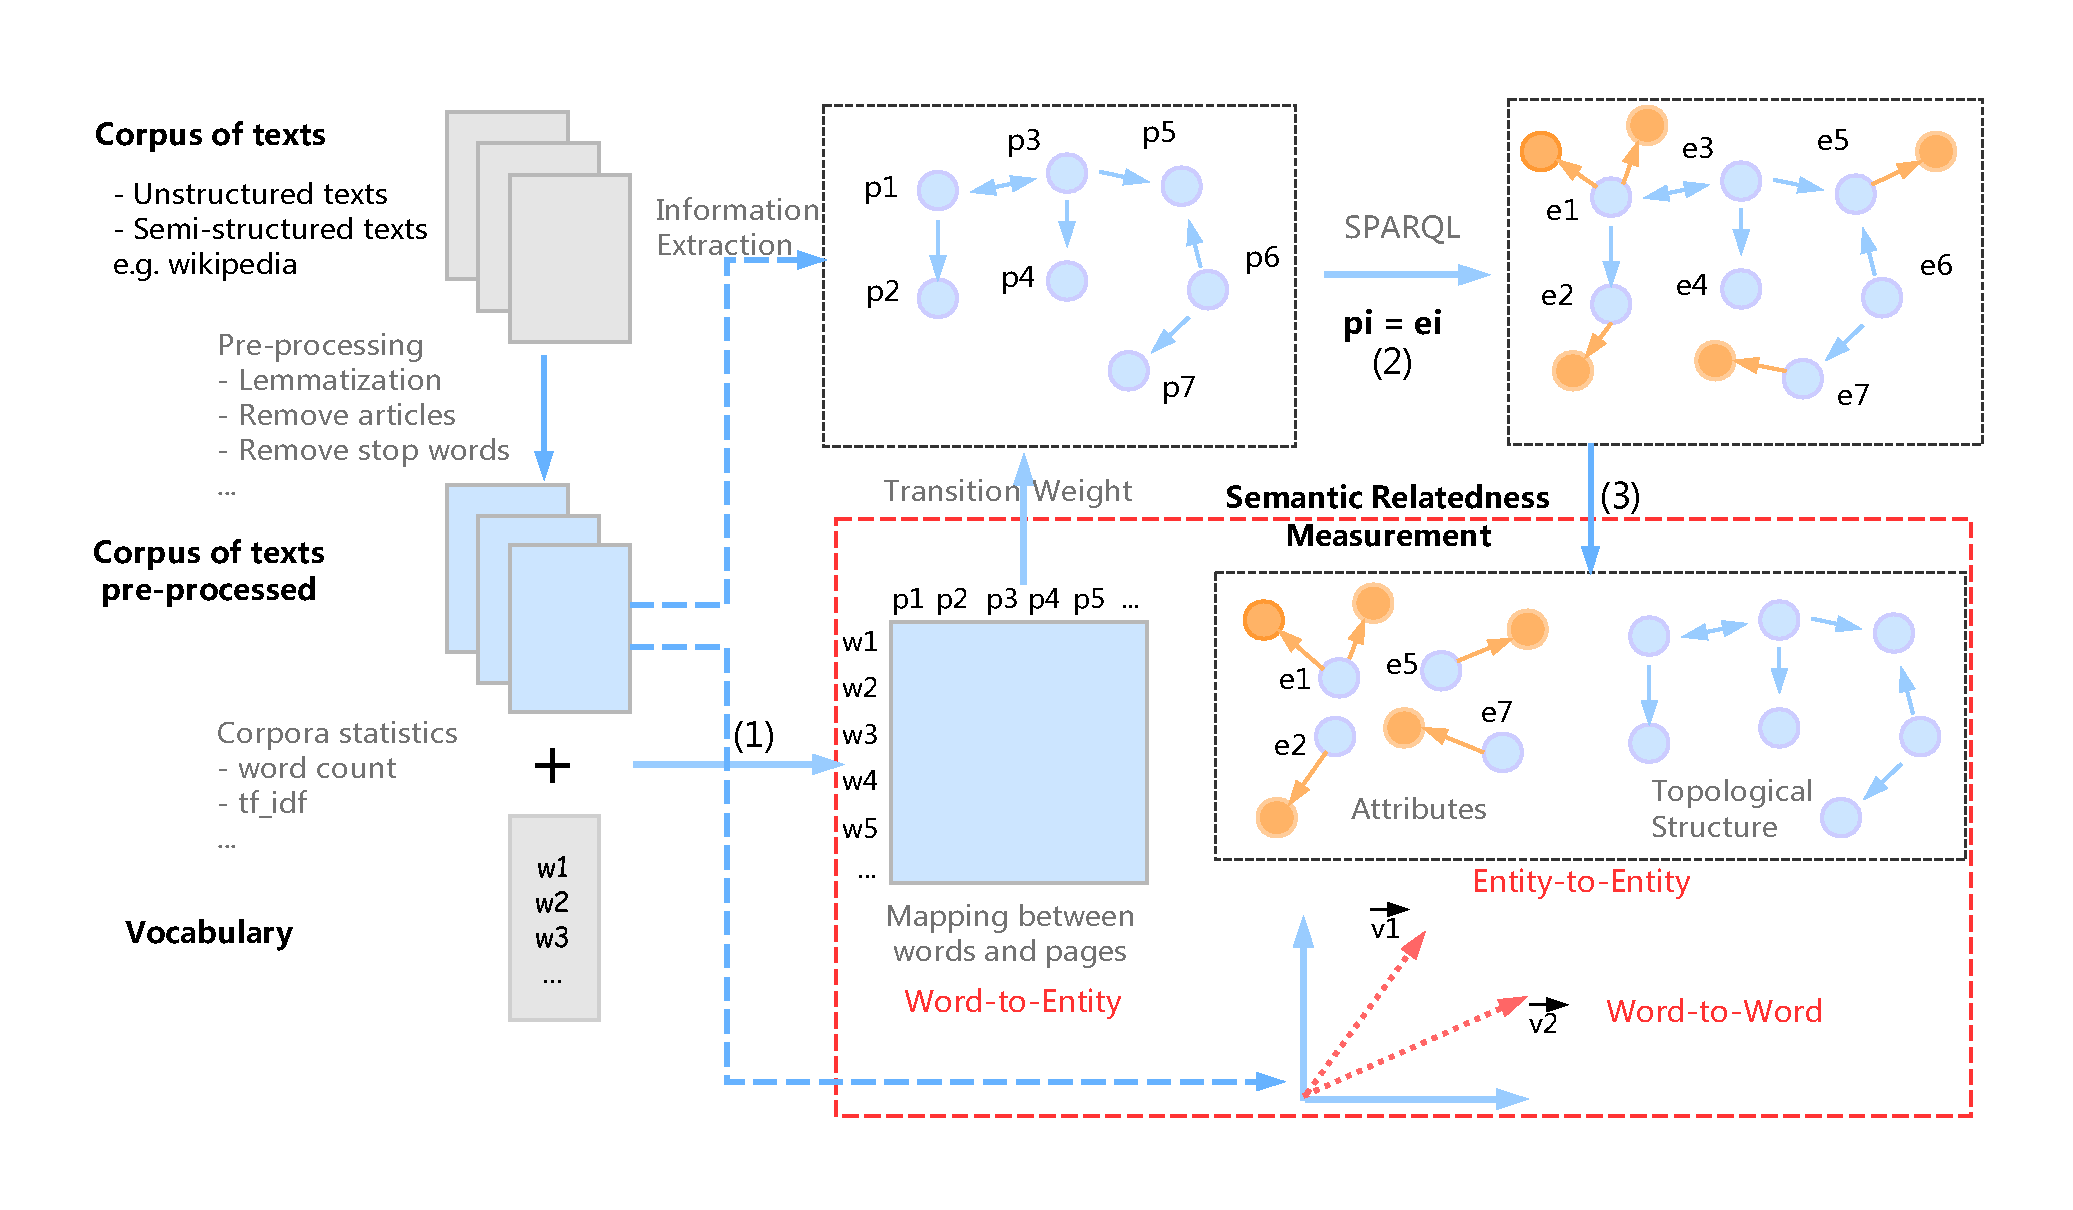
\includegraphics[width=1\textwidth]{chap4-3.pdf}}
    \smallcaption{基于DBpedia中构建的知识关联网络驱动的语义关联度计算流程}
    \label{chap4-3}
\end{figure}

\subsection{词语之间的语义关联度计算}
\label{dbpedia_word2vec}
这部分的处理同本文\ref{word2vec},本节不做赘述。

\subsection{词语与实体之间的的语义关联度计算}
在知识关联网络中,词语层与实体层之间存在着多对多的关系。由于词语的多义性,对于一个给定的词,知识关联网络中存在着多个实体与之对应。为了计算一个词语($w$)与一个实体($e$)之间的关联度,1)一些研究者们将词语与实体之间的共现次数作为其关联度标准~\cite{aaai/Pirro12},但是这种方法对于一些频次较高的常用词不敏感,如\emph{this}、\emph{that}等。2)还有一些研究者从词语的意义角度出发~\cite{aaai/GongXH18},他们认为如果实体$e$是词语$w$的唯一关联实体,则$e$和$w$高度相关联。基于这种假设他们通过链接受欢迎度(Link Popularity,LP)来计算强相关的锚文本词语与其对应的实体之间的关联度:
\begin{equation}
    \label{lp}
    LP(w, e) = \sum_{P}^{ }\sum_{S \in P, w \in S}^{ } \frac{\sum_{w^{'} \in S}^{ }tf\_idf(w^{'},e)}
    {\sum_{e^{'} \in e(w)}^{ }\sum_{w^{'} \in S}^{ }tf\_idf(w^{'}, e^{'})}
\end{equation}
\noindent 其中,$P$代表维基百科的一篇文章,$S$代表$P$中包含词语$w$的句子,$w^{'}$则表示组成句子$S$的词语。$e(w)$表示有锚文本单词$w$外链指向的所有页面集合,即实体集合。这种方法仅仅考虑来锚文本词语与外链页面的关系,忽略了词语与包含该词语的当前页面的关系,本文扩展$e(w)$为:
\begin{equation}
    \label{entities-set}
    e(w) = e_{a}(w) \cup e_{m}(w)
\end{equation}
\noindent 其中$e_{a}(w)$代表了公式\ref{lp} 中的由锚文本指向的实体集合,而$e_{m}(w)$指包含该词的且不是该词对应锚文本指向的实体页面。然后我们提出全受欢迎度(Full Popularity, FP)来计算词语与实体之间的关联度,有:
\begin{equation}
    \label{fp}
    FP(w,e) = \left\{\begin{matrix}
        LP(w,e) & e \in e_{a}(w) & \\
        \frac{tf\_idf(w,e)}{\sum_{e^{'} \in e_m(w)}^{ }tf\_idf(w,e^{'})} & e \in e_{m}(w) & 
        \end{matrix}\right.
\end{equation}
\noindent 最后对于一个词语$w$与实体$e$之间的关联度,有:
\begin{equation}
    \label{f_we}
    f_{we}(w, e) = \frac{FP(w, e)}{\sum_{e^{'} \in e(w)}^{ }FP(w, e^{'})}
\end{equation}


\subsection{实体之间的语义关联度计算}
知识关联网络的实体层本质上表现为多关系图,其中实体的语义信息同时被实体周围的属性信息,以及实体所处的网络拓扑结构所描述。属性信息部分描述了细致的语义关系如A是B的朋友,B是组织C的成员等,而拓扑结构信息则反映了实体间的共现信息中的潜在语义信息。两个实体可能拥有完全不同的属性空间描述,但他们处在相似的网络空间结构中,同样地两个处在不同结构中的实体可能拥有相同的属性空间。在本节提出的模型中,我们采取两种不同的模型分别学习实体在属性空间与拓扑结构空间的分布式向量表示,最后通过加权求和的方式得到实体之间的语义关联度。

\textbf{属性空间嵌入:}对于属性空间的嵌入,最简单直接的方法是\emph{one-hot}编码。这种方法枚举所有属性类型,然后生成一个长度等于属性类型总量的向量,向量中每个元素对应于一个属性。这样对于一个实体的属性空间来说,其拥有的属性对应的向量元素为1,没有的的属性为0,每个实体最后对应的向量长度都等于属性总量。对于DBpedia来说其属性类型总量是百万量级的,\emph{one-hot}编码消耗巨大且效果不好。

对于知识图谱中三元组所描述的明确语义信息,之前很多研究者们将头实体(h)、关系(r)和尾实体(t)这样的关系映射到低维向量空间上的转移操作,认为其对应的向量表示满足下面的关系~\cite{nips/BordesUGWY13, aaai/WuFCABW18}:
\begin{equation}
    \label{hrt}
    \vec h + \vec r \approx \vec t
\end{equation}

\noindent 基于这样的理论,本文将实体属性向量空间表示为$\mathbb{R_a} ^ {N \times d}$,其中假设$N$代表着所有属性实体总量,$d$表示为实体在属性空间的向量维度。我们结合实体以及关系来最小化Margin Ranking损失,即通过最小化正例实体属性对之间间隔,最大化负例实体属性对之间间隔这样的方法来学习其向量表示:
\begin{equation}
    \label{attribute_formula}
    \mathcal{L} = \sum_{(a,b) \in G_{attr}^+}^{ } \sum_{b^- \in G_{attr}^-}^{ }[\ell + cos(a,b)-cos(a,b^-)]_+
\end{equation}

\noindent 公式中$[x]_+=max(0, x)$,$\ell$代表间隔超参数。$G_{attr}$表示由多组\emph{(h, r, t)}三元祖构成的图属性空间,公式中$G_{attr}^+$表示正例三元组构成的图属性空间,$G_{attr}^-$表示负例三元组构成的图属性空间。其中,我们通过下面两种采样策略去得到$G_{attr}^+$:1)正例$a$由头实体h和关系r共同构成,而正例$b$仅包含尾实体t;2)正例$a$仅包含头实体h,正例$b$包含关系r和尾实体t。至于$b^-$则$G_{attr}^-$中表示采样到的负样例,本文采用k-负采样策略~\cite{corr/Mikolov13}在每个批次(batch)更新中去得到k个负样例对。最后我们采用随机梯度下降法(stochastic gradient descent,SGD)去优化公式\ref{attribute_formula}。值得注意的是,每次SGD更新参数的步骤发生在$G_{attr}^+$采样正例并求损失之后。

\textbf{拓扑结构空间嵌入:}
一个实体的拓扑结构空间包含着描述这个实体的潜在语义信息,举个例子来说,当某用户在浏览器中访问到\emph{Apple\_Inc}这个页面时,页面中包含着大量的该用户可能感兴趣的描述其他实体的页面,像\emph{Microsoft\_Windows}或者\emph{Graphical user interface},但是这些实体并不是\emph{Apple\_Inc}的属性实体。为了去考虑这样的隐含信息,之前有很有研究者~\cite{aaai/ZhangZH15, aaai/GongXH18}尝试在Wikipedia语料库中通过文本处理去得到实体间链接这样的语义特征。知识图谱DBpedia中的实体通过关系\emph{WikiPageRedirectOf}被连接,这种关系对应着Wikipedia中页面之间的链接信息。我们记这样的拓扑结构空间为$G_t = G(E, R_{redirect})$,其中$E$代表DBpedia实体集,而$R_{redirect}$代表着由\emph{WikiPageRedirectOf}构成的边集。

显而易见,$G_t$本质上表现为加权图的形式,$R_{redirect}$中的边拥有不同的转移概率。举个例子来说,某用户正在浏览器中浏览Wikipedia的一篇文章\emph{Apple\_Inc},页面中包含着其他几十个相关的文章描述了不同的实体。当该用户想要去了解更多关于{Apple\_Inc}的扩展细节时,该用户一般会首先关注到跟当前页面密切相关的文章。因此,他将会访问相关的Wikipedia页面而忽略掉相关度不高的。由此可见\emph{Apple\_Inc}与其他文章描述的实体间有不同的转移概率,而且这种转移是有方向的,即从A页面到B页面的转移概率和从B页面到A页面的转移概率可能是不同的。

然而,在DBpedia中以三元组存储的关系是无权重的。假定两个实体$e_i$和$e_j$通过关系$r_{ij}$连接,为了给关系$r_{ij}$分配权重,最简单直接的方法是考虑实体$e_i$与$e_j$对应的锚文本之间的共现关系。对于给定实体$e_j$对应的锚文本,我们记为$t_j$,使$cnt(e_i, e_j)$表示实体$e_i$对应的Wikipedia文章中文本$t_j$出现的次数,则基于计数统计的实体间$e_i$和$e_j$转移概率$W_{cnt}(e_i, e_j)$为:
\begin{equation}
    \label{cng_formula}
    W_{cnt}(e_i, e_j) = \frac{cnt(e_i, e_j)}{\sum_{e^{'} \in P_i}^{ }cnt(e_i, e^{'})}
\end{equation}

\noindent 其中$P_i$表示实体$e_i$对应的维基页面,$e^{'}$则是$P_i$中的外链锚文本指向的维基页面描述的实体。然而仅仅考虑锚文本的频率会给予很多高频词更好的权重,然而其与本实体关联度并不高。为了弥补这样的缺点,我们计算$t_j$相对于页面$P_i$的TF-IDF(Term Frequency–Inverse Document Frequency)值作为实体$e_i$到$e_j$转移概率:
\begin{equation}
    \label{w_tf-idf_formula}
    W_{tf\_idf}(e_i, e_j) = \frac{tf\_idf(e_i, e_j)}{\sum_{e^{'} \in P_i}^{ }tf\_idf(e_i, e^{'})}
\end{equation}



经过上述的步骤,我们可以得到加权图$G_t$,为了使图中实体在其拓扑结构空间中是可以比较的,我们需要将其嵌入在更具表达力的低维向量空间。在$G_t$中,拥有相似邻居的节点往往在语义空间中更加接近。本文基于这样的假设来学习实体的向量表征,对于一个实体这需要最大化其邻居节点的观测概率。形式化地说,对于一个给定的实体$e_i$,其邻居节点$(e_0, e_1, ..., e_i, ...e_l)$的观测概率可以表示为条件概率$Pr$:
\begin{equation}
    \label{pr}
    Pr((e_0, e_1, ..., e_{i-1}, e_{i+1}, ..., e_l)|e_i)
\end{equation}

\noindent 之前研究者们已经提出过多种在网络中通过随机游走生成采样序列的方法~\cite{kdd/Perozzi14, kdd/GroverL16},其中node2vec~\cite{kdd/GroverL16}中提出的偏置随机游走通过综合考虑深度优先遍历与广度优先遍历取得了不错的效果,本文也采用这种方法来生成采样序列,并基于下面的策略来进行随机游走:
\begin{equation}
    \label{zeta}
    \zeta_{pq}(t,x) = \left\{\begin{matrix}
        \frac{1}{p} && \text{if} & d_{tx} = 0 & \\
        1           && \text{if} & d_{tx} = 1 & \\
        \frac{1}{q} && \text{if} & d_{tx} = 2 & 
        \end{matrix}\right.
\end{equation} 
\noindent 其中$t$表示上次访问的节点,$x$代表下一个要访问的节点,$d_{tx}$表示节点$t$与节点$x$之间的距离,参数$p$和$q$是两个需要提前设置的参数,用来调控深度优先遍历与广度优先遍历对采样过程的影响。

如图\ref{chap4-4} 所示,对于给定的DBpedia无权图,我们通过上述基于TF-IDF的方法给图中节点之间的关系加权,然后通过公式\ref{zeta}中的偏置随机游走策略生成采样序列。图\ref{chap4-4}右侧子图展示了偏置随机游走的过程,假设我们经过红色节点$t$到达了蓝色节点$v$,接下来可能走向的节点包含$\{t, x_1, x_2\}$,根据节点$t$到到这些节点的距离,对应的偏置权重如图所示,对于$x_1$来说,$d_{tx_1}$的值为2,则$x_1$作为随机游走的下一个节点的概率为原先边的的权重乘上$1/q$,其他节点类似。

\begin{figure}[!ht]
    \centerline{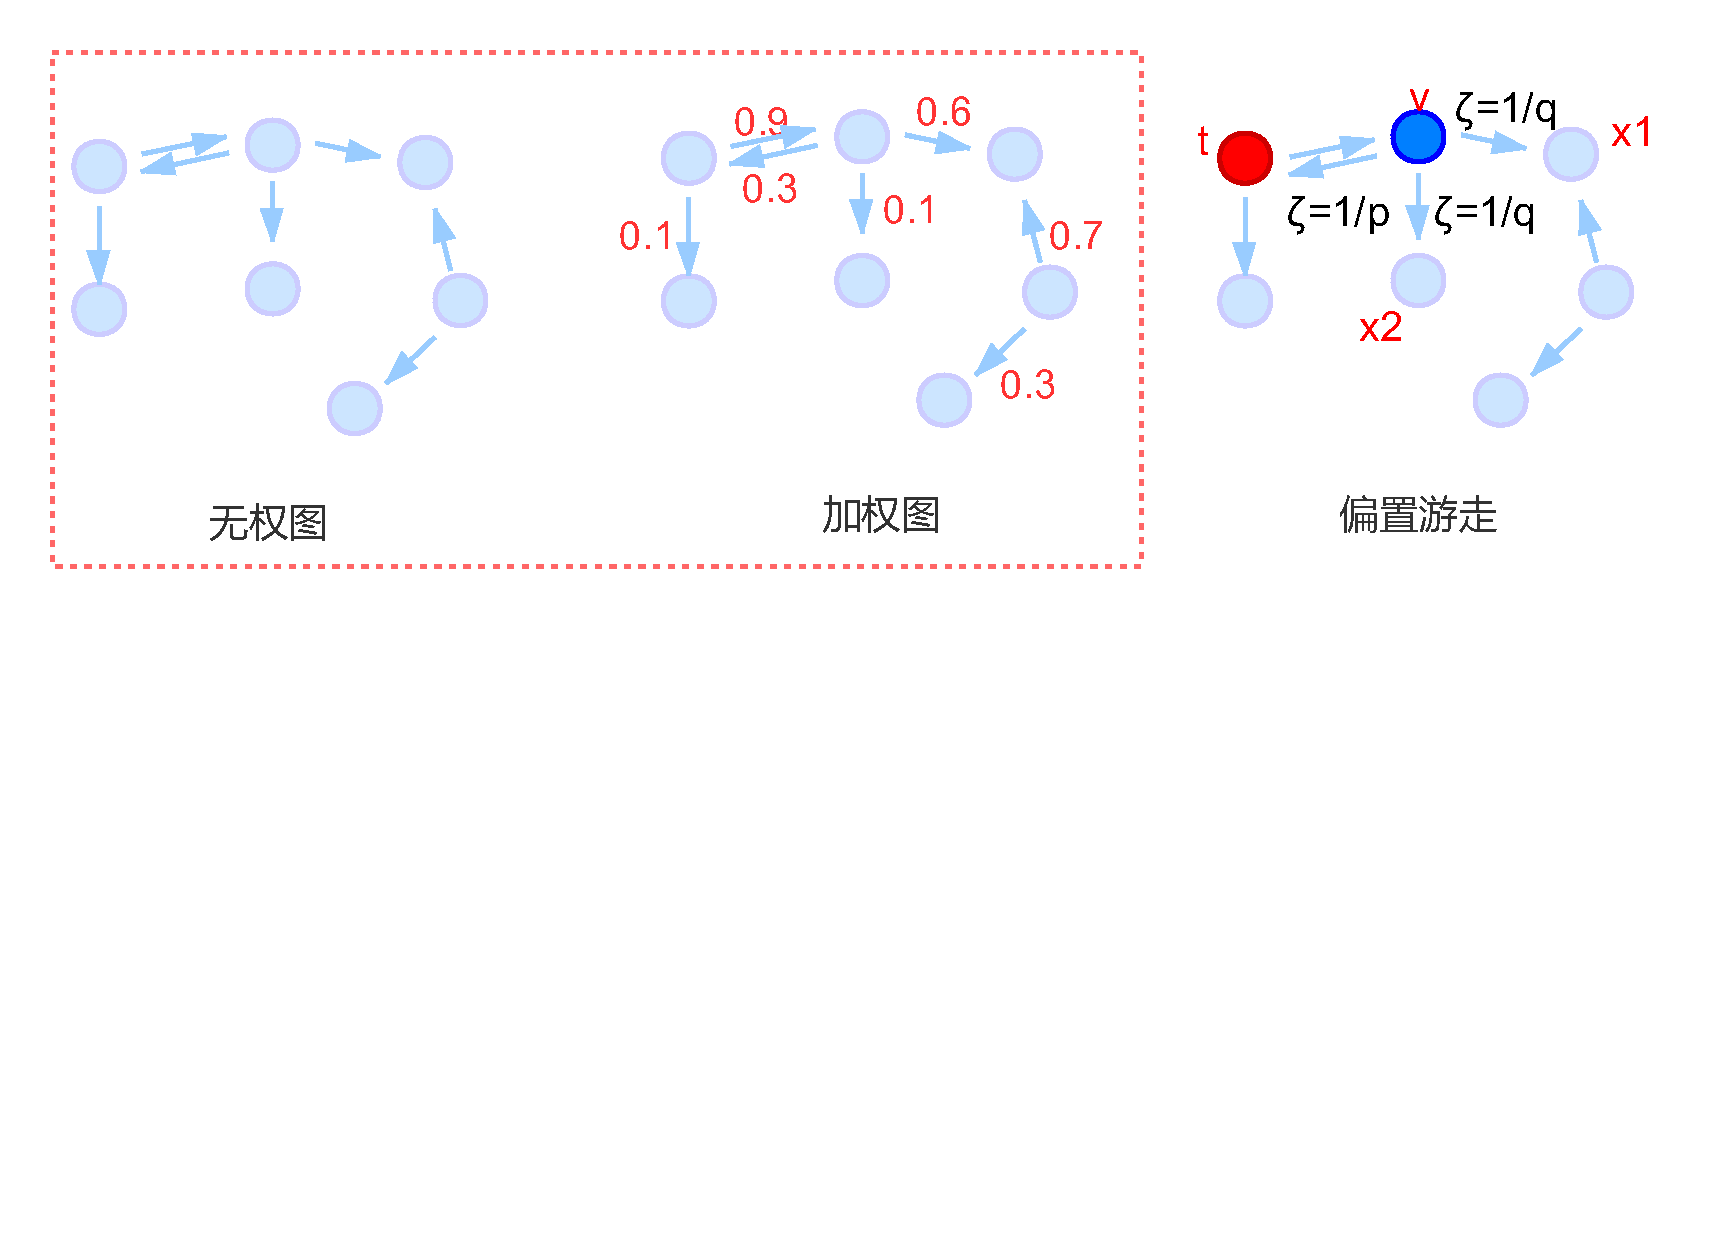
\includegraphics[width=1\textwidth]{chap4-4.pdf}}
    \smallcaption{加权图与随机游走采样示例}
    \label{chap4-4}
\end{figure}

当得到采样序列后,我们的目标是在向量空间最大化给定节点在序列中的邻居节点的观测概率,即最大化公式\ref{pr}。我们给出一个将实体映射到向量空间的函数:$\Phi: e \in E \rightarrow \mathbb{R_t}^{\left | E \right | \times d}$。其中$E$是图$G_t$中包含的所有实体,$\Phi$是一个$\left | E \right | \times d$规模的可训练的矩阵参数。通过这样的映射关系,对于$E$中每一个实体$e_i$,我们通过最小化下面的损失函数可以得到一个d维的向量,
\begin{equation}
    \label{log_pr}
    minimize\ -log Pr(N(e_i)|\Phi(e_i)) = -log\prod_{e^{'} \in N(e_i)}^{ }Pr(e^{'}|\Phi(e_i))
\end{equation}

\noindent 其中$Pr(e^{'}|\Phi(e_i))$表示在目标向量空间中实体$e^{'}$作为$e_i$出现的概率。对于$e_i$邻居$N(e_i)$中的每一个实体$e^{'}$,我们通过\emph{softmax}函数对其进行归一化处理可以得到:
\begin{equation}
    Pr(e^{'}|\Phi(e_i)) = \frac{exp(\Phi(e^{'})\cdot \Phi(e_i))}{\sum_{e_k \in N(e_i)}^{ }exp(\Phi(e_k)\cdot \Phi(e_i))}
\end{equation}
\noindent 对于实体拓扑空间的嵌入,我们通过随机梯度下降法来优化公式\ref{log_pr}。

\textbf{实体层语义关联度:}
通过对实体的潜在语义信息进行学习,将其映射到向量空间,我们可以得到实体的属性空间向量表征$\vec {va}_i$与拓扑结构空间的向量表征$\vec {vt}_i$,然后通过组合两者有:
\begin{equation}
    \label{d_f_e}
    f_e(e_i, e_j) = \alpha cos({\vec {va}_i, \vec {va}_j}) 
    + (1-\alpha)cos(\vec {vt}_i,\vec {vt}_j)
\end{equation}
\noindent $\alpha$作为权重参数,取值范围为$[0,1]$,衡量了实体的属性空间与拓扑结构空间关联度对最后结构的影响。

\subsection{语义关联度计算}
在上述计算的基础上,我们采取公式\ref{F_e_avg}来计算实体层的语义关联度,并按照章节\ref{chap02-sr}中所述的语义关联度计算算法来计算语义关联度,然后我们将其公式\ref{d_f_e}带入公式\ref{F},即可得到最后的词语间关联度值。值得注意的是,在这部分计算中,我们没有采用基于取最大值的策略来衡量实体层语义关联度,这是因为词语与实体之间的权重分布,会使单条词语到实体的连接路径权重范围不在[0,1]之间,因此取最大值的策略在这部分不适合。

\section{本章小结}

在本章节,我们首先简要介绍了DBpedia,然后提出基于DBpedia构建的知识关联网络。其中词语与实体的对应关系,本文综合考虑文本外链与文章对词语的影响来计算词语与实体的关联度。最后我们提出一种实体嵌入方法,综合学习实体周围的属性信息及其网络结构的拓扑信息。

  \chapter{实验设计与结果分析}
\label{chap:chap05}

本章介绍了语义关联度的评测数据与评测标准,并在此基础上展开实验,通过与多种基准模型的对比,分别验证了基于WordNet和DBpedia构建的知识关联网络驱动的语义关联度计算模型的性能。

\section{评测标准与实验数据}
\subsection{评测数据}

\begin{table*}[htbp]
    \center
    \smallcaption{MC30: 人为标注的词语间关联度数据示例}
    \vspace{5pt}
    \begin{tabular}{p{2cm}p{2cm}p{1.4cm}p{2cm}p{2cm}p{1.4cm}}
    \hline
    \multicolumn{2}{l}{词对}     & 标注值          & \multicolumn{2}{l}{词对}     & 标注值  \\ \hline
    automobile    &    car    &    3.92 & gem    &    jewel    &    3.84  \\ \hline 
    journey    &    voyage    &    3.84 & boy    &    lad    &    3.76  \\ \hline 
    coast    &    shore    &    3.70 & asylum    &    madhouse    &    3.61  \\ \hline 
    magician    &    wizard    &    3.50 & midday    &    noon    &    3.42  \\ \hline 
    furnace    &    stove    &    3.11 & food    &    fruit    &    3.08  \\ \hline 
    bird    &    cock    &    3.05 & bird    &    crane    &    2.97  \\ \hline 
    implement    &    tool    &    2.95 & brother    &    monk    &    2.82  \\ \hline 
    brother    &    lad    &    1.66 & crane    &    implement    &    1.68  \\ \hline 
    car    &    journey    &    1.16 & monk    &    oracle    &    1.10  \\ \hline 
    cemetery    &    woodland    &    0.95 & food    &    rooster    &    0.89  \\ \hline 
    coast    &    hill    &    0.87 & forest    &    graveyard    &    0.84  \\ \hline 
    shore    &    woodland    &    0.63 & monk    &    slave    &    0.55  \\ \hline 
    coast    &    forest    &    0.42 & lad    &    wizard    &    0.42  \\ \hline 
    cord    &    smile    &    0.13 & glass    &    magician    &    0.11  \\ \hline 
    rooster    &    voyage    &    0.08 & noon    &    string    &    0.08  \\ \hline 
    \end{tabular}
    \label{mc30}
\end{table*}

词语间语义关联度度量是一个十分主观的事情,不同的人基于略有差异的认知,会得到不同的结果。为了方便研究者们的研究,不少语言学家和心理学家提出了很多人工标注的基准数据集~\cite{MC30/Miller02, RG65/RubensteinG65, wordsim353/FinkelsteinGMRSWR02, ws/AgirreAHKPS09, YP130/Yang06verbsimilarity, MEN/BruniTB14},本文列举了以往研究者常用的三种数据集的信息,并且本文利用这三种数据集作为模型的评价数据集合:
\begin{enumerate}
    \item RG65~\cite{RG65/RubensteinG65}:RG65作为经典的数据集,常用来作为语义相似度度量的标准数据集,其中包含有65对英文名词。对于每对词语,受试者们给出一个在$[0,4]$之间的相关度值然后取平均值作为最后的评分,该评分越高,两个词相似度越高,反之亦然。
    \item MC30~\cite{MC30/Miller02}:MC30是RG65中的一个子集,由于时间的迁移,RG65中一些词的相关性发生了变化,研究者重新评分其部分子集来构成了MC30,如表格~\ref{mc30}所示,本文给出了其全部示例。
    \item WS353~\cite{wordsim353/FinkelsteinGMRSWR02}:WS353中包含353对英文单词,其词性包含名词、动词以及形容词,是常用的词语间语义关联度度量的评测数据。词对间关联度评分取值范围为$[0,10]$,值越大,两个单词关联度越高。
\end{enumerate}
最后在表格~\ref{golden},本文整理并给出本文所使用的评测数据集及其简要信息。

\begin{table}[htbp]
    \center
    \smallcaption{词语间语义关联度评测数据集}
    \vspace{5pt}
    \begin{tabular}{|p{1.8cm}|p{1.8cm}|p{1.8cm}|p{5cm}|}
    \hline
    数据名称    & 词对数量    & 取值范围      & 引文 \\ \hline
    RG        & 65         & [0,4]       & Rubenstein\&Goodenough1965       \\ \hline
    MC        & 30         & [0,4]       & Miller\&Charles1991          \\ \hline 
    WS353     & 353        & [0,10]      & Finkelstein et al.2002         \\ \hline
    \end{tabular}
    \label{golden}
\end{table}

\subsection{评测标准}
不同评测数据集的关联度标注值取值范围不同,无法通过简单的距离计算来衡量模型表现。同之前的语义关联度计算研究一样,本文采用模型估计值与评测数据标准值之间的相关系数来衡量模型表现。两组变量的相关系数反映了两组变量之间在统计关系上的相关程度,其取值范围一般是$[-1, 1]$,取值越大相关程度越高,其中-1表示两组变量负相关,1则表示正相关。下面给出了本文中使用的三种相关系数及其简要介绍:

\begin{enumerate}
    \item 皮尔森(Pearson)相关系数:本文被记为$\gamma$,反映了两组变量之间的线性相关程度,当一组变量的变化与另一组变量的变化成比例相关时,这两个变量具有线性关系。其计算公式如下:
    \begin{equation}
        \label{pearson}
        \gamma(X, Y) = \frac{E[(X-\mu_X)(Y-\mu_Y)]}{\sigma_X \sigma_Y}
    \end{equation}
    \noindent 其中分子部分构成了$X$和$Y$的协方差,$E(\cdot)$表示求一组变量的期望值,$\mu_X$和$\mu_Y$分别表示两组变量$X$和$Y$的平均值,$\sigma_X$和$\sigma_Y$则分别表示两组变量的标准差。
    \item 斯皮尔曼秩(Spearman's rank)相关系数:本文被记为$\rho$,反映了两组变量的移动方向是否一致。斯皮尔曼秩相关系数检验的不是数据之间的关系,而是数据排名之间的关系,这对于数据异常值和数据规模具有更强的鲁棒性。其计算过程往往需要先对原始数据排序,对于两组原始变量$X$和$Y$,排序后得到$rg_X$和$rg_Y$,然后通过下面的公式来计算其相关系数值:
    \begin{equation}
        \label{spearman}
        \rho(X, Y) = \gamma(rg_X, rg_Y) =  \frac{E[(rg_X-\mu_{rg_X})(rg_Y-\mu_{rg_Y})]}{\sigma_{rg_X} \sigma_{rg_Y}}
    \end{equation}
    \noindent 其中符号含义类比公式~\ref{pearson}。可见,当两组变量排序前后相对顺序一致时,斯皮尔曼秩相关系数等于皮尔森相关系数。
    \item 皮尔森相关系数与斯皮尔曼秩相关系数的调和平均(Harmonic mean)相关系数:这部分本文取皮尔森相关系数与斯皮尔曼秩相关系数的调和平均值作为最后的评价指标,公式如下。
    \begin{equation}
        \label{harmonic}
        \mu(X, Y) = \frac{2\gamma(X, Y)\rho(X, Y)}{\gamma(X, Y)+\rho(X, Y)}
    \end{equation}
\end{enumerate}

\subsection{实验数据}

\textbf{基于WordNet构建的知识关联网络:}
基于WordNet构建知识关联网络时,本文采用的版本是WordNet 3.1。本文首先遍历其中所有同义词集即实体,抽取出每个实体周围的三种关系:上位关系(hypernyms)、下位关系(hyponyms)以及部分整体关系(member holonyms),组成知识关联网络中实体层之间的关系,其中节点与边规模如表格~\ref{wordnet_data}~所示。由表中数据可见实体之间的关系比较稀疏。

\begin{table}[htbp]
    \center
    \smallcaption{WordNet实体及其边规模信息}
    \vspace{5pt}
    \begin{tabular}{|p{1.6cm}|p{1.6cm}|p{1.6cm}|p{2.5cm}|p{1.6cm}|}
    \hline
    实体   & 上位关系 & 下位关系 & 部分整体关系 & 边总数   \\ \hline
    117,660   & 89,090 & 89,090 & 12,294 & 190,474    \\ \hline
    \end{tabular}
    \label{wordnet_data}
\end{table}

\textbf{基于DBpedia构建的知识关联网络:}
基于DBpedia构建知识关联网络的过程中,要通过Wikipedia页面信息建立起词语与实体之间的关系。本文采用维基百科2016年10月份的备份数据\footnote{https://dumps.wikimedia.your.org/},并通过简单的文本分析建立起词语与维基百科之间的联系,然后再通过文章独有的数字ID建立起与DBpedia中实体之间的关系。其中Wikipedia与DBpedia的实体规模信息如表格~\ref{wiki_data}~所示。

之前本文提到Wikipedia中的实体与DBpedia中一一对应,表格~\ref{wiki_data}~中所示DBpedia中的实体数量要多于Wikipedia中页面所描述的实体数。这是因为DBpedia不仅仅包含了从Wikipedia中抽取的实体,也连接了其他语义信息库如原语库、YAGO知识图谱等等。
在连接Wikipedia页面与词语时,本文首先要对Wikipedia的语料库做简单的预处理。本文移除了文本中的停用词与标点符号,忽略了其中包含单词数少于50的页面,同时对于其中一些用处较少的命名空间(namespace)如分类(Category)、文件(File)以及模板(Template),\footnote{https://en.wikipedia.org/wiki/Wikipedia:Namespace}本文不予考虑。

% \renewcommand\arraystretch{1.2}
\begin{table}[htbp]
    \center
    \smallcaption{Wikipedia和DBPedia信息}
    \vspace{5pt}
    \begin{tabular}{|p{2cm}|p{2cm}|p{2cm}|p{2cm}|}
    \hline
              & 实体数    & 日期        \\ \hline
    Wikipedia & 5.5M     & 2016-10     \\ \hline
    DBPedia   & 6.6M     & 2016-10     \\ \hline
    \end{tabular}
    \label{wiki_data}
\end{table}


\section{知识关联网络驱动的语义关联度计算模型评估}
此节分别给出基于WordNet和DBpedia构建的知识关联网络中遇到的模型参数设置,以及模型在标准评测数据集上的表现。

\subsection{基于WordNet构建的知识关联网络}
\textbf{参数设置:}
在基于WordNet构建的知识关联网络中,本文基于自注意力机制学习到实体的向量表示,其中模型的参数设置如下:
\begin{itemize}
    \item 在实体层,本文采用两层的自注意力模型来训练实体向量表示。第一层的输入为WordNet中实体所对应的词向量的平均值,输出维度为256,多头注意力值$K=4$,采用拼接的方式组合学习到的4个实体向量表示。而第二层输出维度256,$K=4$,然后取4个实体向量的平均值,作为最后的实体向量表示输出。
    \item 训练自注意力模型时,本文采用Adam算法来优化目标函数,其中初始学习率设置为0.01,权重衰减值(weight\_decay)设置为0。
\end{itemize}


\begin{table*}[htbp]
    \center
    \smallcaption{不同网络嵌入模型在实体层语义关联度计算上的相关系数表现:皮尔森-$\lambda$, 斯皮尔曼秩-$\rho$, 调和平均-$\mu$相关系数}
    \vspace{5pt}
    \begin{tabular}{|l|c|c|c|c|c|c|c|c|c|c|}
    \hline
    \multirow{2}{*}{图嵌入模型}     & \multirow{2}{*}{策略} & \multicolumn{3}{c|}{$\lambda$} & \multicolumn{3}{c|}{$\rho$} & \multicolumn{3}{c|}{$\mu$} \\ \cline{3-11} 
     &
       &
      \multicolumn{1}{c|}{\textbf{MC}} &
      \multicolumn{1}{c|}{\textbf{RG}} &
      \multicolumn{1}{c|}{\textbf{WS}} &
      \multicolumn{1}{c|}{\textbf{MC}} &
      \multicolumn{1}{c|}{\textbf{RG}} &
      \multicolumn{1}{c|}{\textbf{WS}} &
      \multicolumn{1}{c|}{\textbf{MC}} &
      \multicolumn{1}{c|}{\textbf{RG}} &
      \multicolumn{1}{c|}{\textbf{WS}} \\ \hline
    \multirow{2}{*}{node2vec} &
      max &
      \multicolumn{1}{c|}{0.535} &
      \multicolumn{1}{c|}{0.618} &
      \multicolumn{1}{c|}{-0.049} &
      \multicolumn{1}{c|}{0.344} &
      \multicolumn{1}{c|}{0.461} &
      \multicolumn{1}{c|}{-0.093} &
      \multicolumn{1}{c|}{0.419} &
      \multicolumn{1}{c|}{0.528} &
      \multicolumn{1}{c|}{-0.064} \\ \cline{2-11} 
                               & mean & 0.142 & 0.263 & -0.001 & 0.197 & 0.320 & -0.039 & 0.165 & 0.289 & -0.002 \\ \hline
    \multirow{2}{*}{GraphSage} & max  & 0.872 & 0.808 & 0.421 & 0.833 & 0.799 & 0.173 & 0.852 & 0.803 & 0.245 \\ \cline{2-11} 
                               & mean & 0.706 & 0.637 & 0.464 & 0.661 & 0.641 & 0.458 & 0.683  & 0.639 & 0.461 \\ \hline
    \multirow{2}{*}{Un-GAT}       & max  & $\bf 0.913$ & $\bf 0.848$ & 0.435 & $\bf 0.845$ & $\bf 0.816$ & 0.397 & $\bf 0.878$  & $\bf 0.832$ & 0.415 \\ \cline{2-11} 
                               & mean & 0.632 & 0.662 & $\bf 0.549$ & 0.635 & 0.652 & $\bf 0.515$ & 0.633 & 0.657 & $\bf 0.531$ \\ \hline
    \end{tabular}
    \label{table5-5}
\end{table*}


\textbf{模型表现:}
WordNet中存储了描述词语不同含义的同义实体集,这些实体之间的相关程度可以反映不同单词之间的关联性。回顾章节\ref{chap:chap03}中描述的基于WordNet构建的知识关联网络,其表现为有向无权图。为了丰富词语层的关联程度,本文在图注意力网络(GAT)的基础上,采用无监督训练的方式训练得到实体向量表示。在表格~\ref{table5-5}~中,本文基于三种基准评测数据集,给出了三种网络嵌入模型在实体层之间的关联程度$F_e(w_i, w_j)$(见前文公式~\ref{F_e}~)上的相关系数表现。其中$max$和$mean$分别对应于章节\ref{chap:chap03}中提到的计算实体层语义关联度的两种策略,对比模型的参数设置如下:
\begin{itemize}
    \item node2vec~\cite{kdd/GroverL16}是一种基于随机游走的无监督图嵌入模型,对于其提出的偏置随机游走策略,本文在公式~\ref{zeta}~中有过详细介绍。在本章节的对比实验中,本文设置其中的两个参数$p$和$q$均为1,游走长度为50,邻居窗口大小为10,对每个节点随机游走其相关序列采样10次。优化器采用Adam,其中学习率设置为0.01,权重衰减设置为0.0005。模型输出实体向量维度设置为256。
    \item GraphSage~\cite{nips/HamiltonYL17}是一种基于神经网络的图嵌入模型,这种模型通过不同的聚合算子来综合考虑固定邻居特征对当前节点的影响。本文采用基于平均策略的两层的GraphSage来进行实验,第一层和第二层的向量输出维度均设置为256,其中对于每个节点,其邻居采样大小设置为5。模型优化器设置为Adam,其中学习率为0.01,权重衰减值为0。
\end{itemize}

基于上述模型参数设置,从表格~\ref{table5-5}~中可以看出,基于$max$的策略取实体集之间的最大关联度作为计算结果,要比取平均值的$mean$策略效果要好很多。这在一定程度上也符合人类判断直觉,当两个词的某个意思关联度比较高而其他含义相关度不高时,人们常常认为两个词是相关的。此外,从表格~\ref{table5-5}~中还可以看出,基于图注意力网络的无监督训练得到结果取得了最好的效果,即可以更好地表征实体的语义特征。接下来本文将介绍基于图注意力网络的无监督训练与词语层关联度度量对最终结果的影响。

\begin{figure}[htbp]
    \begin{minipage}{0.48\textwidth}
      \centering
      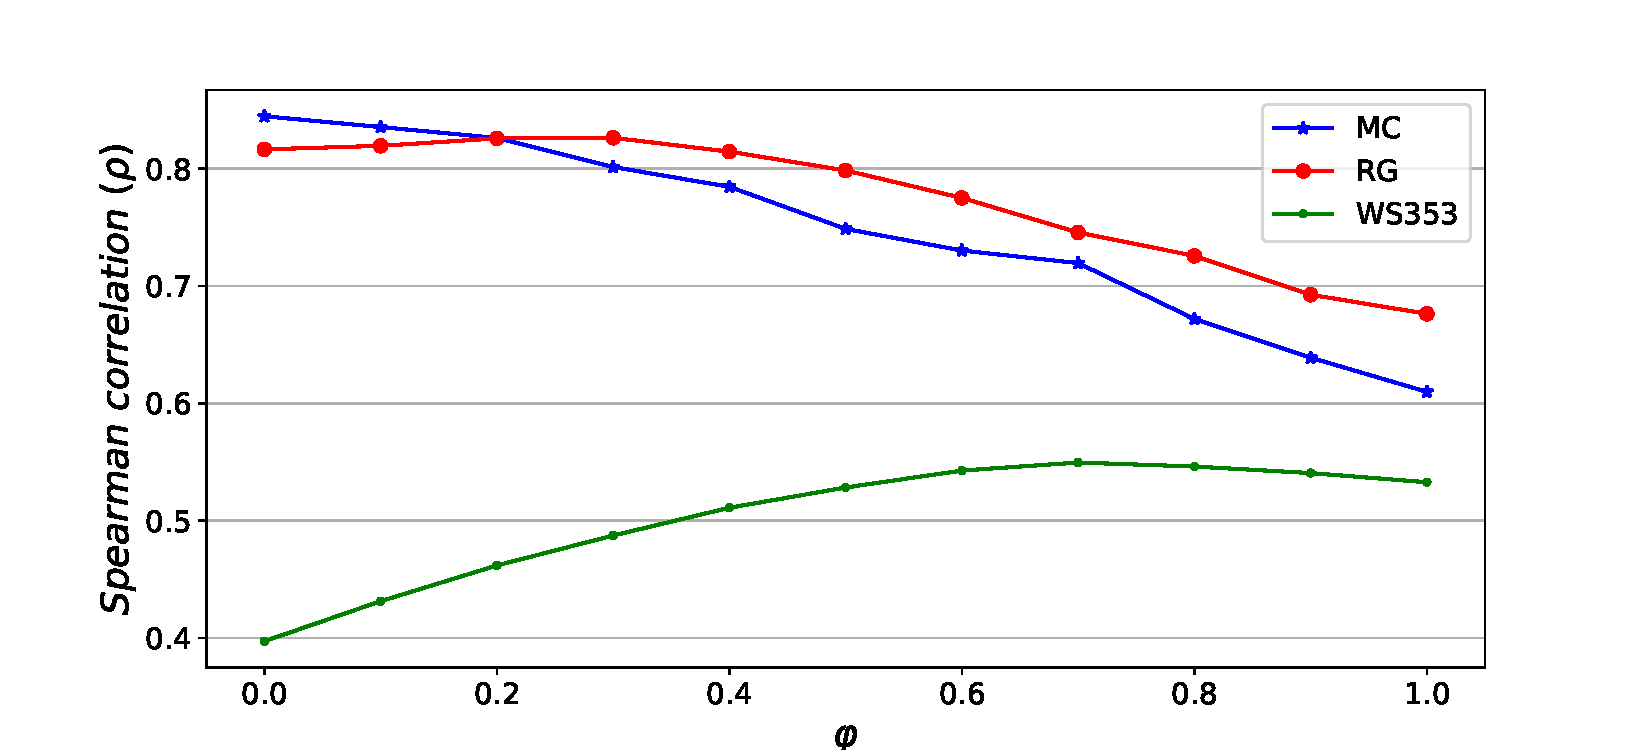
\includegraphics[width=1\textwidth]{params_lambda_w_max.pdf}
      \smallcaption{基于max策略的语义关联度计算中$\lambda$参数对于模型表现的影响}
      \label{fig:lambda_w_max}
    \end{minipage}\hfill
    \begin{minipage}{0.48\textwidth}
      \centering
      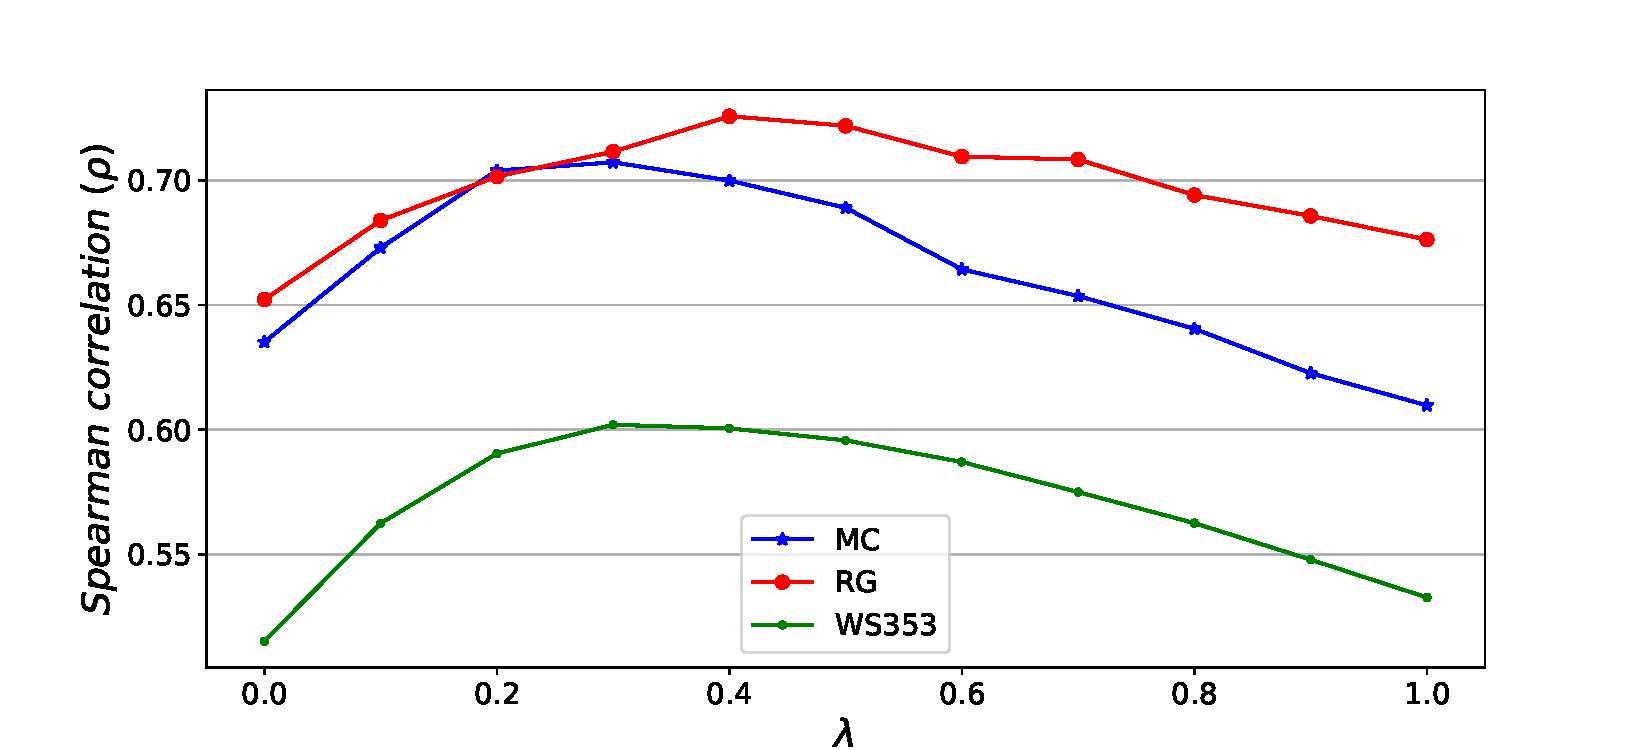
\includegraphics[width=1\textwidth]{params_lambda_w_mean.pdf}
      \smallcaption{基于mean策略的语义关联度计算中$\lambda$参数对于模型表现的影响}
      \label{fig:lambda_w_mean}
    \end{minipage}
    \label{fig:wordnet_sr}
\end{figure}

前文提到的参数$\varphi$用来权衡词语层关联度与实体层关联度对最终语义关联度的影响,如图\ref{fig:lambda_w_max}和图\ref{fig:lambda_w_mean},基于自注意力机制的网络嵌入下的不同实体层关联度方式,本文给出了$\varphi$对最终结果的影响。从图\ref{fig:lambda_w_max}可以看出在基于max策略的实体层关联度度量模型中,对于MC和RG这两个数据集,$\varphi$取$0$时的效果最好。这是因为本文在网络输入初始化的时候,采用的是实体相关联的词向量平均值作为输入,这在一定程度上已经考虑了从文本中训练得到的语义向量信息,而WordNet知识关联网络嵌入则起到了学习词语背后相关联实体的语义内容的作用,可以看出最后结果要比单纯文本训练词向量的结果要好。而对于WS这个数据集,当$\varphi$取$0.8$时,模型效果最优,词语层关联度起主要贡献。另外在图\ref{fig:lambda_w_mean}基于mean策略的中,知识关联网络嵌入中学习到的实体语义信息被平均弱化,表现不如基于max的策略。但是当$\varphi$取$0.3$的时候,网络嵌入学习得到的语义信息还是可以为词向量补充语义信息。

\subsection{基于DBpedia构建的知识关联网络}
\textbf{参数设置:}
在基于DBpedia构建的知识关联网络中,需要确定的模型参数如下:
\begin{itemize}
    \item 在~\ref{dbpedia_word2vec}~中,本文在处理后的Wikipedia语料库上训练Word2Vec模型,在这部分,本文采用100维向量输出, 30窗口大小以及Skip-gram model与negative sampling的结合来训练得到词向量。
    \item 在实体层属性空间嵌入部分,本文设置间隔margin $\ell=0.05$, 输出维度 $d=100$, 负采样数 $k=50$, 本文还设置随机梯度下降的学习率为$0.01$来优化Margin Ranking损失。
    \item 在实体层网络拓扑结构空间嵌入部分,本文采用Skip-gram模型来训练随机采样的序列,其中偏置随机游走中$p$和$q$的值分别设置为0.7和0.3,同时本文采用100维的输出维度, 10的窗口大小来训练模型。
\end{itemize}


\begin{table*}[htbp]
    \center
    \smallcaption{不同的权重分配策略构建的知识关联网络在三种数据集上的皮尔森-$\lambda$, 斯皮尔曼秩-$\rho$, 调和平均-$\mu$相关系数}
    \vspace{5pt}
    \begin{tabular}{|l|c|c|c|c|c|c|c|c|c|}
    \hline
    \multirow{2}{*}{模型} & \multicolumn{3}{c|}{$\lambda$}     & \multicolumn{3}{c|}{$\rho$}          & \multicolumn{3}{c|}{$\mu$} \\ \cline{2-10} 
                           & \textbf{MC}&\textbf{RG}&\textbf{WS} & \textbf{MC}&\textbf{RG}&\textbf{WS} & \textbf{MC}&\textbf{RG}&\textbf{WS}\\ \hline
    $KAN_{cnt}$            & 0.850 & 0.826 & 0.630 & 0.836 & 0.805 & 0.633 & 0.842 & 0.816 & 0.631   \\ \hline
    $KAN_{tf\_idf}$        & $\bf 0.892$  & $\bf 0.887$ & $\bf 0.783$ & $\bf 0.866$ & $\bf 0.861$ & $\bf 0.835$ & $\bf 0.879$ & $\bf 0.874$ & $\bf 0.808$ \\ \hline
    \end{tabular}
    \label{table5-6}
\end{table*}


\textbf{模型表现:}
回顾\ref{subsec4-3-3}节实体层之间的关联度度量,对于实体所处的拓扑结构空间,本文采用两种策略来为实体之间的关系分配权重:1)$W_{cnt}(e_i,e_j)$表示实体$e_i$与实体$e_j$对应的锚文本之间的共现频率;2)$W_{tf\_idf}(e_i,e_j)$评估了实体$e_j$的锚文本相对于$e_i$所对应文章的重要程度。基于这两种评价策略,本文分别构造得到两种知识关联网络$KAN_{cnt}$以及$KAN_{tf\_idf}$。从表格~\ref{table5-6}~中可以看出,基于$KAN_{tf\_idf}$的语义关联度度量模型在不同评测数据集上表现都更加好。这是因为$TF-IDF$适当的调节了文章中的关键词词频,通过考虑逆文档频率降低了高频通用词的权重,使得词语与文档之间的关联度度量更准确。

前文提到的参数$\alpha$用来平衡属性空间关联度与拓扑结构空间关联度之间的权重。为了得到最优的模型表现和提高模型鲁棒性,本文不在最终评测数据集上调节参数,而是选择在数据集\emph{WS-Rel}~\cite{ws/AgirreAHKPS09}试验参数$\alpha$对最终结果的影响。\emph{WS-Rel}中包含有252个单词对以及关联度评分值,这个数据集在很多关联度数据集中没有被使用。图~\ref{fig:alpha}~展示了不同的$\alpha$取值对最后Spearman相关系数($\rho$)的影响,可以看出当$\alpha$趋近于0.5的时候,$\rho$取值最大,这意味着属性空间的语义信息与拓扑结构中所包含的隐含语义信息对语义关联度的计算有着相同的共现。

另一个参数$\varphi$起到权衡知识关联网络中实体层$F_e$与词语层语义关联度$F_w$的作用。图~\ref{fig:lambda}~展示了$F_e$和$F_w$对在最终评测数据集上对最终语义关联度计算的影响,可见当$\varphi=0.2$时,Spearman相关系数$\rho$取值达到最大。显然,$F_w$对最后的语义关联度计算影响更大,起到了主导的作用,而$F_e$中包含的隐含语义信息也有效的丰富了词语的语义空间,使得最终的关联度计算值有所提升。

\begin{figure}[htbp]
    \begin{minipage}{0.48\textwidth}
      \centering
      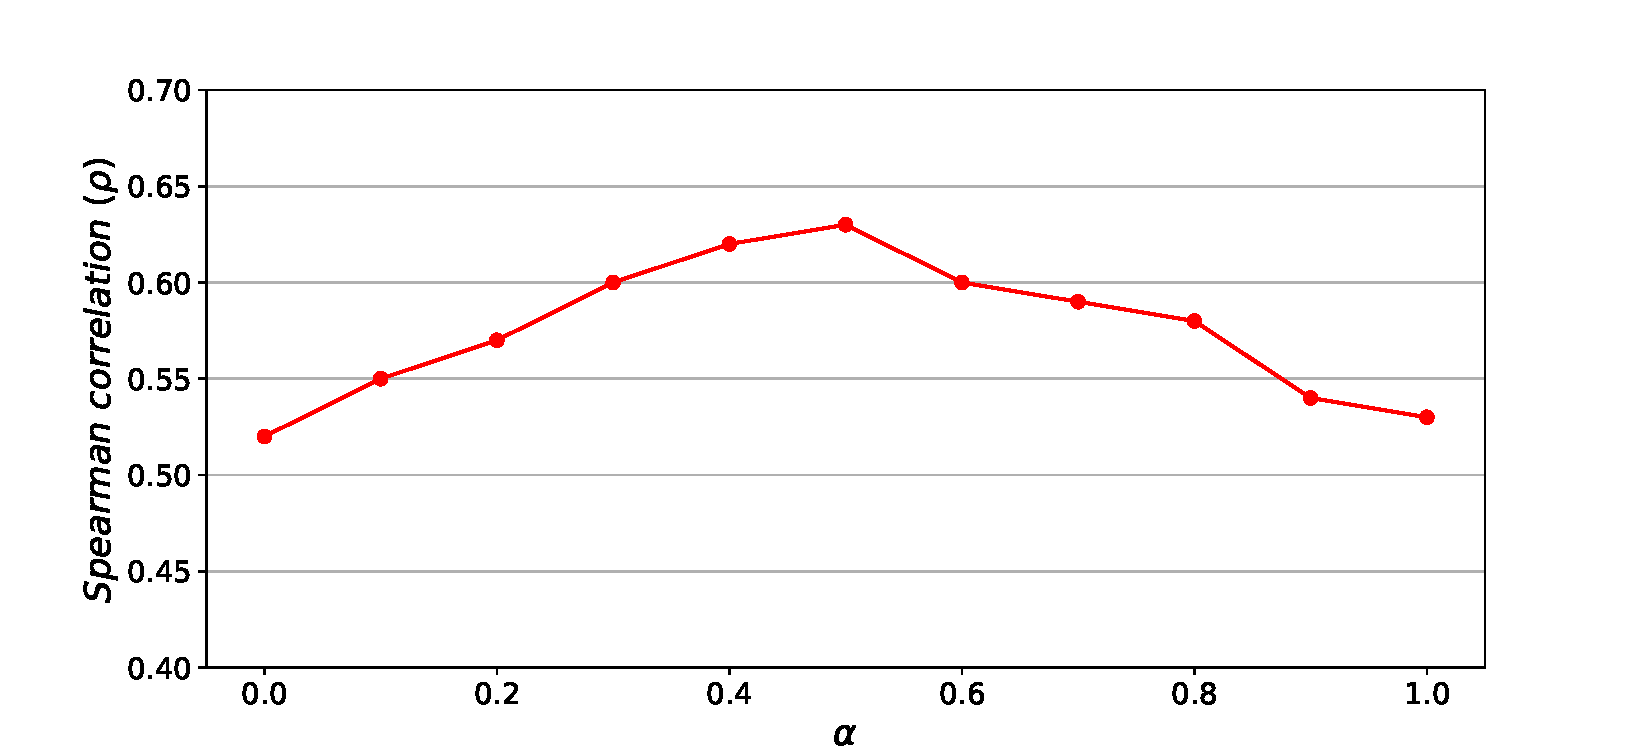
\includegraphics[width=1\textwidth]{params_alpha.pdf}
      \smallcaption{$\alpha$对实体层之间关联度的影响}
      \label{fig:alpha}
    \end{minipage}\hfill
    \begin{minipage}{0.48\textwidth}
      \centering
      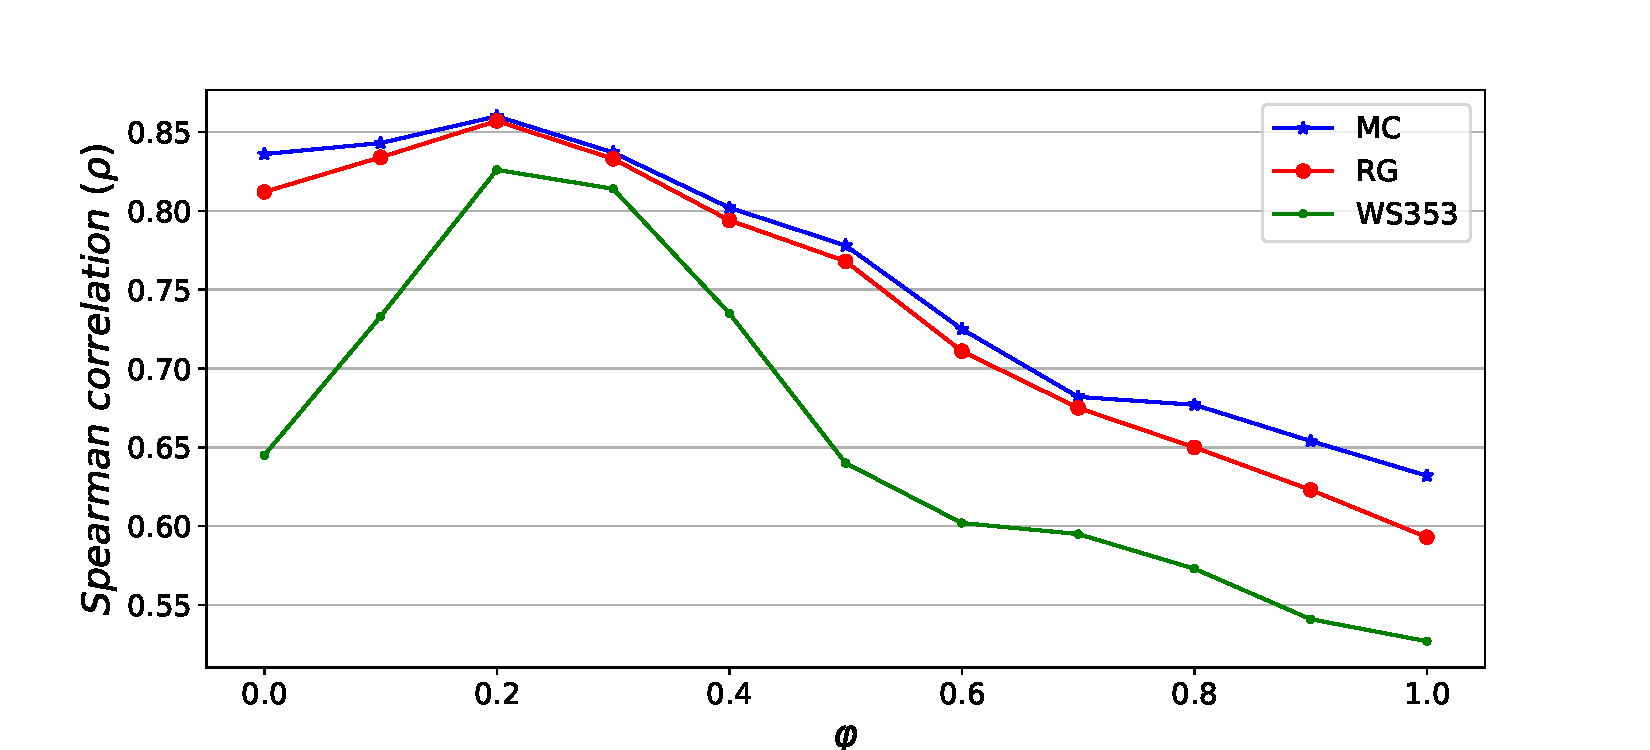
\includegraphics[width=1\textwidth]{params_lambda_d.pdf}
      \smallcaption{$\lambda$参数对于模型表现的影响}
      \label{fig:lambda}
    \end{minipage}
\end{figure}


\section{模型的对比与分析}
此节基于表格\ref{golden}中提到的三种人为标注的高质量语义关联度数据,对比了传统语义关联度计算模型与本文提出的知识关联网络驱动的计算模型之间的差异,并分析了多种模型之间的差异。

\textbf{对比模型:}
基于标准评估数据,本文主要对比了以下几种语义关联度计算模型论文中的报告结果:
\begin{itemize}
    \item 基于共现原则的方法:ESA\cite{aaai/StrubeP06}中则采用$tf-idf$技术来为文本中的词语分配权重,然后利用词语对应的文本中包含的词语$tf-idf$权重向量来计算语义关联度;SSA\cite{aaai/HassanM11}中利用维基百科中词语上下文中的实体信息为词语构建语义画像,然后通过基于规则的方法计算词语间关联度;Word2Vec\cite{corr/Mikolov13}利用词语之间的共现信息来将词语表征在向量空间,由此来计算语义关联度;SaSA\cite{aaai/WuG15}利用维基百科中词语对应的不同实体,在词义层面学习得到词语向量表示,解决了Word2Vec中无法表征词语多义性的缺点。
    \item 基于关联网络的方法:AN\cite{aaai/ZhangZH15}和HAN\cite{aaai/GongXH18}提出关联网络的概念来连接词语与知识库实体之间的关系,然后综合考察了词语层与实体层的语义关联度。
\end{itemize}

本文中提出的模型中被作为对比的是:
\begin{itemize}
    \item 基于WordNet构建的知识关联网路驱动的语义关联度计算:在这部分实体层向量学习中,采用基于网络注意力机制的方法取得了较好的结果,这里记基于这种机制的语义计算模型为$WordNet\_KAN_{gat}$,取$\varphi=0$的结果作为对比结果。
    \item 基于DBpedia构建的知识关联网路驱动的语义关联度计算:这部分中,基于$tf-idf$的实体层网络取得了最优的结果,我们记基于这种方法的语义计算模型为$DBpedia\_KAN_{tf\_idf}$,取$\varphi=0.2$的结果作为对比结果。
\end{itemize}


\begin{table*}[htbp]
    \center
    \smallcaption{不同语义关联度计算模型在三种数据集上的皮尔森-$\lambda$, 斯皮尔曼秩-$\rho$, 调和平均-$\mu$相关系数}
    \vspace{5pt}
    \begin{tabular}{|l|c|c|c|c|c|c|c|c|c|}
    \hline
    \multirow{2}{*}{模型} & \multicolumn{3}{c|}{$\lambda$}     & \multicolumn{3}{c|}{$\rho$}          & \multicolumn{3}{c|}{$\mu$} \\ \cline{2-10} 
                           & \textbf{MC}&\textbf{RG}&\textbf{WS} & \textbf{MC}&\textbf{RG}&\textbf{WS} & \textbf{MC}&\textbf{RG}&\textbf{WS}\\ \hline
    ESA                    & 0.588 &  - -  & 0.503 & 0.727 &  - -  & 0.748 & 0.650 &  - - & 0.602    \\ \hline
    SSA                    & 0.879 & 0.861 & 0.590 & 0.843 & 0.833 & 0.604 & 0.861 & 0.847 & 0.597   \\ \hline
    Word2Vec               & 0.852 & 0.834 & 0.633 & 0.836 & 0.812 & 0.645 & 0.844 & 0.823 & 0.639   \\ \hline
    SaSA                   & 0.886 & 0.882 & 0.733 & 0.855 & 0.851 & 0.739 & 0.870 & 0.866 & 0.736   \\ \hline
    $AN_{wiki}$            & 0.865 & 0.858 & 0.740 & 0.848 & 0.843 & 0.813 & 0.856 & 0.850 & 0.775   \\ \hline
    $HAN_{wiki}$           & 0.886 & 0.884 & 0.772 & 0.860 & 0.857 & 0.826 & 0.873 & 0.870 & 0.798   \\ \hline
    $WordNet\_KAN_{gat}$   & $\bf 0.913$ & 0.848 & 0.435 & 0.845 & 0.816 & 0.397 & 0.878  & 0.823 & 0.570 \\ \hline
    $DBpedia\_KAN_{tf\_idf}$        & 0.892 & $\bf 0.887$ & $\bf 0.783$ & $\bf 0.866$ & $\bf 0.861$ & $\bf 0.835$ & $\bf 0.879$ & $\bf 0.874$ & $\bf 0.808$ \\ \hline
    \end{tabular}
    \label{table5-7}
\end{table*}

\textbf{模型表现的对比与分析:}
表格~\ref{table5-7}~给出了本文提出的两种模型以及多种对比模型在MC30、RG65以及WS353三种数据集上的相关系数表现。
从表格中可以看出,传统基于关联网络的方法$AN_{wiki}$和$HAN_{wiki}$通过关联词语与语料库文档的关系,更好地捕捉到了词语的语义特征,改善了传统基于共现的方法的缺点。本文提出的模型中,基于WordNet的语义关联度计算模型$WordNet\_KAN_{gat}$仅在MC30数据集上的表现优于$AN_{wiki}$和$HAN_{wiki}$,这是因为WordNet中仅仅存储了实体之间的相对关系与位置信息,相对于文本库中抽取得到的手工特征显得表现力不足。而基于DBpedia的语义关联度计算模型$DBpedia\_KAN_{tf\_idf}$弥补了这个缺点,同时考虑了实体所处的属性空间与拓扑结构空间,向量化的表示也使本文的模型更加灵活,更具表达力。


\section{本章小结}
本章基于传统评测数据,对测评标准进行了介绍。对于基于WordNet构建的知识关联网络,本章对比了多种网络嵌入模型的表现,验证了基于自注意力机制的无监督网络嵌入模型的效果。对于基于DBpedia构建的知识关联网络,本章对比了实体层实体属性空间与拓扑空间语义信息对最后关联度度量结果的影响。最后通过与传统基准模型的对比,验证了本文提出的模型的效果。

  \chapter{总结与展望}
\label{chap:chap07}

\section{全文总结}

所谓词语间语义关联度计算,是指对于给定的一对词语,研究者们采用合适的方法,结合不同的背景知识,给出一个数值来表示两个词语在语义空间上的关联程度。这是一项基础且十分重要的任务,在自然语言处理、推荐系统和计算机视觉方面都有相关的应用。经典的计算方法主要利用了隐含在词典库(WordNet)或文本语料(Wikipedia)中的隐含语义关系,他们或在词典树上基于距离关系,或在Wikipedia中基于共现原则来衡量两个词之间的相似程度,得了不错的效果。然而这些方法忽略了隐含在词语背后的语义网络,近年来,新提出的基于自由关联网络的方法改善了这个缺点,在语义关联度计算方面取得了更好的效果。但是这种方法需要事先对Wikipedia进行大量的复杂的预处理,此外,这种方法采用了固定的评分函数来衡量Wikipedia页面之间的相关性,这造成了模型灵活性和表达能力的欠缺。因此,本文提出知识关联网络来学习更加灵活鲁棒的知识表示,由此改良语义关联度计算的表现,具体来讲,本文的研究内容包含下面几个部分。
\begin{enumerate}
    \item 本文基于WordNet、DBpedia知识库去构建了知识关联网络,同时考虑了词语与词语、词语与实体以及实体与实体之间的关系对语义关联度度量的影响。
    \item 在知识关联网络的实体层,针对不同的网络结构,ben wen提出了不同的网络嵌入模型。在基于WordNet构建的网路中,ben wen将图注意力机制应用到无监督表示学习中;在基于DBpedia构建的网络中,ben wen同时考虑了实体属性空间与拓扑空间的语义信息。这些分布式向量表示方法在扩展性与灵活性上要明显优于传统模型中的基于规则的比较函数。
    \item 基于标准语义关联度度量数据集的实验证明,ben wen的模型要优于几种对比模型,取得了更好的效果。
\end{enumerate}

\section{工作展望}
本文对于知识关联网络驱动语义关联度计算进行了深入的研究,针对不同的知识库,本文采用不同的模型来学习实体向量表征,取得了不错的效果。但是本文的工作仍然有需要改进的地方:
\begin{enumerate}
    \item 本文通过网络嵌入方法将词语背后关联的实体语义信息转化为分布式向量,可以起到丰富词语语义特征的作用。但是对于自然语言处理的其他任务,比如文本分类、关键词抽取等任务,添加词语背后的语义特征是否起作用仍需要实验验证。
    \item 在基于WordNet构建的知识关联网络中,本文采用的基于自注意力机制的无监督学习虽然取得了不错的效果,但是网络嵌入过程相比传统的Node2vec模型训练过程比较慢,无法迁移到大规模图上。在未来的工作中,我们将考虑对大规模图上的嵌入方法进行深入研究。
    \item 在基于DBpedia构建的知识关联网络中,对于一个给定的单词,跟其相关度比较高的的往往只有几个实体,大部分实体只是简单的包含该单词,这部分实体构成噪音实体。在未来的工作中,我们考察采用实体背后所对应的抽象分类(Category)图来减少图的规模,提高词语关联度比较的速度与性能。
\end{enumerate}

%%%%%%%%%%%%%%%%%%%%%%%%%%%%%%
%% 附件部分
%%%%%%%%%%%%%%%%%%%%%%%%%%%%%%
%\backmatter

  \xiaosihao

  % 参考文献
  \kaishu
  \bibliographystyle{sudabst}
  \bibliography{../bib/ref}

  \songti

  %发表文章目录
  % \begin{publications}{99}
% \end{publications}

% \begin{center}
% \textbf{会议论文}
% \end{center}

% [1] \textbf{Jiapeng Li}, Wei Chen, Binbin Gu, Junhua Fang, Zhixu Li, Lei Zhao*: Measuring Semantic Relatedness with Knowledge Association Network. 23rd International Conference on Database Systems for Advanced Applications DASFAA, 2019, April 22-25, Chiang Mai, Thailand, pp 676-691.(EI,CCF B 类,已发表)



% \begin{center}
% \textbf{期刊论文}
% \end{center}

% [1] \textbf{Jiapeng Li}, Wei Chen, An Liu, Zhixu Li, Lei Zhao*: FTS: a feature-preserving trajectory synthesis model.GeoInformatica, 2018, pp 49-70.(SCI,CCF B 类,已发表)

\begin{publications}{99}

\item \textbf{Jiapeng Li}, Wei Chen, Binbin Gu, Junhua Fang, Zhixu Li, Lei Zhao*: Measuring Semantic Relatedness with Knowledge Association Network. 23rd International Conference on Database Systems for Advanced Applications DASFAA, 2019, April 22-25, Chiang Mai, Thailand, pp 676-691.(EI,CCF B 类)


\item \textbf{Jiapeng Li}, Wei Chen, An Liu, Zhixu Li, Lei Zhao*: FTS: a feature-preserving trajectory synthesis model.GeoInformatica, 22 volume, 2018, pp 49-70.(SCI,CCF B 类)

\end{publications}


  % 致谢
  \newpage
  \thispagestyle{empty}
  \setThanksStyle
  \begin{thanks}
    犹记得七年前在苏州大学入学时的场景,十八岁的年纪,对接下来的大学生活无限憧憬。七年里,走了几千个日夜的晴岚路,看了几万次的尊师轩,好的坏的,希望的不希望的,时时刻刻在天赐庄校区发生着,彼时遥远的告别的日子也悄悄靠近着。在苏州大学计算机科学与技术学院的日子里,仿佛升级打怪,学习、考试、敲代码、赶论文。从一个敲键盘就都费劲的菜鸟逐渐成长到一名合格的硕士研究生。这七年来,感谢所有老师同学在工作生活中给予我的帮助和启发。

    衷心感谢七年的大学生涯里导师赵雷老师从各个方面对我的教导。大一上学期学习C语言课程的时候,认识了您,并在大一结束的时候加入您组内,加入先进数据分析实验室。一路走来,太多回忆,亦师亦友,熬夜赶论文时,生活陷入困难时,思想困惑时,生病住院时等等,您都给了太多太多的帮助,谆谆教诲,时刻谨记。十分有幸、十分高兴能在大学生涯中选择您作为我的导师。谢谢您!

    感谢先进数据分析实验室李直旭老师和陈伟老师对我的帮助,在我研究任务遇到困难时,感谢您们对我一次又一次的指导,使我顺利完成研究任务。感谢师兄朱杰、师姐绪艳霞从本科以来对我的帮助和指导,帮助我找到适合我自己的职业规划。感谢七年舍友夏劲夫和他的女朋友杨慧萍以及李茂龙、葛新越、周欣长久以来的帮助和陪伴。在我研一下学期生病住院时,感谢实验室各位同学的探望和陪伴。谢谢大家。

    感谢我的家人,我的父亲母亲、妹妹、小姨长久以来的的陪伴。正是因为有了你们的陪伴,才有了更好的自己。谢谢大家。

    最后,感谢各位老师在百忙之中评审我的论文,感谢您们的批评和指导。

\begin{flushright}
李佳鹏\qquad\qquad\qquad\qquad  \\
二〇二〇年二月十四日  \\
\end{flushright}

\end{thanks}


\end{document}
